\chapter[The verbal clause]{The verbal clause}\label{ch:8}
\is{Clause!verbal|(}
A verbal clause consists of a verb phrase and optional nominal arguments and adjuncts. The number of arguments depends on the verb; different classes of verbs are discussed in \sectref{sec:3.4.1}. 

The verb phrase has been discussed in Chapter 7; the present chapter focuses on the other core constituents of verbal clauses: the arguments of the verb. The chapter is dominated by two main topics: constituent order and argument marking. These two are inextricably linked – the way arguments are marked, depends on their position in the clause – so they will be discussed together; the discussion will focus on the factors determining the marking of subject and object. 

Constituent order and argument marking are discussed in sections \sectref{sec:8.1}–\ref{sec:8.7}. \sectref{sec:8.1} provides a brief introduction and discusses basic and marked constituent orders. \sectref{sec:8.2} introduces the topic of case-marking, comparing the situation in Rapa Nui with other Polynesian languages. The next sections deal with S/A marking (\sectref{sec:8.3}) and O marking (\sectref{sec:8.4}), respectively. \sectref{sec:8.5} discusses passivisation\is{Passive} and passive-like constructions. \sectref{sec:8.6} discusses a variety of constructions involving non-standard constituent orders and/or non-canonical marking of arguments, e.g. topicalisation and instrumental marking. \sectref{sec:8.7} deals with case marking in nominalised clauses. 

The last sections deal with miscellaneous constituents, some of which are not restricted to verbal clauses, but which are nevertheless included in this chapter: oblique arguments (\sectref{sec:8.8}), reflexives and reciprocals (\sectref{sec:8.9}), comitative\is{Comitative} constructions (\sectref{sec:8.10}) and vocatives (\sectref{sec:8.11}). 

Finally, \sectref{sec:8.12} discusses causativisation, a process which affects the argument structure of the verb and the expression of arguments. 

\section{Introduction; constituent order}\label{sec:8.1}
\is{Constituent order|(}
\is{Object|(}\is{Subject|(}
As pointed out above, most of this chapter will be concerned with the order of constituents and the marking of S, A and O arguments.\footnote{\label{fn:379}See Footnote \ref{fn:109} on p.~\pageref{fn:109} on the terms S, A and O. In this grammar, any clause in which an O argument is either expressed or implied, is counted as transitive\is{Verb!transitive} (regardless other arguments); a clause without an expressed or implied O is considered intransitive (cf. (\ref{ex:3.84}–\ref{ex:3.86}) on p.~\pageref{ex:3.84})\is{Verb!intransitive}. Verbs with a nominalised verb\is{Verb!nominalised} as complement are counted as transitive\is{Verb!transitive}; verbs with a subordinate clause as complement are counted as intransitive\is{Verb!intransitive}.}  A preliminary question concerns the expression of these arguments as such. The verb phrase is the only obligatory element in the verbal clause: any argument can be omitted if its identity is understood from the context. In discourse, both S/A and O are usually left implicit when they are identical to a constituent in the previous clause. An example in which both A and O are implied, is the following:

\ea\label{ex:8.1}
\gll He moko ki muri i tū vi{\ꞌ}e era ko Māhina \textbf{he} \textbf{ha{\ꞌ}i}.\\
\textsc{ntr} rush to near at \textsc{dem} woman \textsc{dist} \textsc{prom} Mahina \textsc{ntr} embrace\\

\glt 
‘He rushed toward that woman Mahina and (he) embraced (her).’ \textstyleExampleref{[R399.191]} 
\z

\tabref{tab:55} shows how often arguments are expressed or not expressed in a corpus of selected texts.\footnote{\label{fn:380}For the analysis of clause structure and case marking, I used a subcorpus of 15 older texts (pre-1940) and 14 newer texts (post-1970). This corpus contains 7807 verbal clauses (2373 in old texts, 5434 in new texts): 2686 transitive\is{Verb!transitive} (including three-argument verbs), 4879 intransitive\is{Verb!intransitive} and 242 with zero valency.} The top part gives figures for intransitive clauses (i.e. clauses in which only one core argument is expressed or implied), the bottom part for transitive clauses (i.e. clauses in which both an A and an O argument are expressed or implied).

\begin{table}[p]
\begin{tabularx}{\textwidth}{Xrr@{\hspace*{1.5cm}} rr@{\hspace*{1.5cm}} rr}

\lsptoprule
 & \multicolumn{2}{l}{~old texts} & \multicolumn{2}{l}{~~new texts} & \multicolumn{2}{l}{~~~~total}\\
\midrule
\\
{intransitive}\is{Verb!intransitive} &  & (1468)&  & (3411)  & & (4879)\\
\midrule
no S &  52.1\%&  (765)&  52.2\%&  (1780)&  52.2\%&  (2545)\\
S &  47.9\%&  (703)&  47.8\%&  (1631)&  47.8\%&  (2345)\\
\\

{transitive}\is{Verb!transitive} &  &  { (852)}&  &  { (1834)}&  &  { (2686)}\\
\midrule
no A, no O &  31.8\%&  (271)&  28.9\%&  (530)&  29.8\%&  (801)\\
A only &  4.6\%&  (39)&  9.1\%&  (167)&  7.7\%&  (206)\\
O only &  51.6\%&  (440)&  45.0\%&  (826)&  47.1\%&  (1266)\\
{A + O} &  12.0\%&  (102)&  17.0\%&  (311)&  15.4\%&  (413)\\
\lspbottomrule
\end{tabularx}
\caption{Expression and non-expression of arguments}
\label{tab:55}
\end{table}

This table shows that in 47.8\% of all intransitive\is{Verb!intransitive} clauses, the argument is expressed. Of the transitive\is{Verb!transitive} clauses, only 7.7+15.4=23.1\% have an overt A, while 47.1+15.4=62.5\% have an overt O. In only 15.4\% of all clauses are both arguments expressed, while in 29.8\% of the clauses neither argument is expressed. 

\is{Constituent order}The default constituent order is VS/VAO. This order is by far the most common one and pragmatically unmarked. Other orders are not uncommon, though. \tabref{tab:56} gives frequencies for all possible constituent orders. Part 1 represents clauses only containing an S/A argument; part 2 represents transitive\is{Verb!transitive} clauses only containing an O argument; part 3 represents transitive clauses with two overt arguments.

\begin{table}[p]
\begin{tabularx}{\textwidth}{Xlrr@{\hspace*{1.5cm}} rr@{\hspace*{1.5cm}} rr}
\lsptoprule
&  & \multicolumn{2}{l}{ {~old texts}} & \multicolumn{2}{l}{ { new texts}} & \multicolumn{2}{l}{ {~~total}} \\
\midrule
{ 1} & { V S/A} &  93.4\%&  (693)&  82.9\%&  (1491)&  86.0\%&  (2184)\\
& { S/A V} &  6.6\%&  (49)&  17.1\%&  (307)&  14.0\%&  (356)\\
\tablevspace
{ 2} & { V O} &  98.2\%&  (432)&  95.8\%&  (791)&  96.6\%&  (1221)\\
& { O V} &  1.8\%&  (8)&  4.2\%&  (35)&  3.4\%&  (43)\\
\tablevspace
{ 3} & { V A O} &  69.6\%&  (71)&  65.3\%&  (203)&  66.3\%&  (274)\\
& { A V O} &  16.7\%&  (17)&  21.9\%&  (68)&  20.6\%&  (85)\\
& { V O A} &  10.8\%&  (11)&  4.8\%&  (15)&  6.3\%&  (26)\\
& { O V A} &  2.9\%&  (3)&  4.8\%&  (15)&  4.4\%&  (18)\\
& { A O V} &  0.0\%&  (0)&  1.9\%&  (6)&  1.5\%&  (6)\\
& { O A V} &  0.0\%&  (0)&  1.3\%&  (4)&  1.0\%&  (4)\\
\lspbottomrule
\end{tabularx}
\caption{Frequencies of constituent orders}
\label{tab:56}
\end{table}

As this table shows, there is a strong preference for verb-initial clauses,\footnote{\label{fn:381}These data do not confirm Fischer’s suggestion (\citealt[323]{Fischer2001Hispan} that SVO is becoming the new unmarked word order (under influence of \ili{Spanish}). It is true that new texts show a higher proportion of SV(O) clauses than old texts; however, it is also true that OV has become more common in new texts. The former may be under \ili{Spanish} influence, but these shifts also suggest a move towards a more flexible syntax, in which a greater variety of constructions becomes common.} but it is not uncommon for S/A to precede the verb (S/AV, AVO, AOV, OAV). It is less common for the object to precede the subject (VOA, OVA, OAV), while clauses in which the object precedes the verb (OV, OVA, AOV, OAV) are rare.\footnote{\label{fn:382}The following example, an actor-emphatic\is{Actor-emphatic construction} construction with \is{Object!preverbal}preposed object, is an example of OAV order (other orders will be exemplified in detail in the following sections):
\ea
\gll ¿Mo aha {\ob}te {\ꞌ}uha\,{\cb}\textsubscript{\textup{O}} {\ob}{\ꞌ}ā{\ꞌ}au\,{\cb}\textsubscript{\textup{A}} i tiaŋi ai?\\
   for what {\db}\textsc{art} chicken {\db}\textsc{poss.2sg.a} \textsc{pfv} kill \textsc{pvp}\\
   \glt 
  ‘Why did you kill the chicken?’ (R250.164)\z 
  } 

Constituent order can be formulated as a set of three constraints: 

%\setcounter{listWWviiiNumviiileveli}{0}
\begin{enumerate}
\item 
V—S/A: the verb precedes the subject;

\item 
A—O: the subject precedes the object; 

\item 
V—O: the verb precedes the object. 

\end{enumerate}

Constituent orders which violate only one constraint (like AVO) are more common than orders violating two or three constraints (like OAV). The statistics above also show that constraint 3 is strongest, while 1 is weakest: in clauses with both arguments expressed (413 total), constraint 1 is violated 95x, constraint 2 is violated 48x, constraint 3 is violated 28x.

There are various motivations for non-VAO constituent orders. S/A and O may be preposed as clause topic or because they are thematic (\sectref{sec:8.6.1}–\ref{sec:8.6.2}); S/A may be preposed in focus in the actor-emphatic construction (\sectref{sec:8.6.3}). Preverbal S/A also occurs after various clause-initial elements (\sectref{sec:8.6.1.1}).

Motivations for the reversal of A and O (i.e. VOA) are also diverse. Some VOA clauses are cases of passivisation\is{Passive} (\sectref{sec:8.5.1}), in other cases the reasons for the marked order are less clear. 
\is{Constituent order|)}

\section{Case marking: introduction}\label{sec:8.2}
\is{Case marking|(}\subsection{Case in Polynesian}\label{sec:8.2.1}

In Polynesian languages, nouns are not inflected for case. As far as case is marked, it is marked by prepositions. The subject of an intransitive\is{Verb!intransitive} clause is usually unmarked, i.e. not preceded by a case-marking preposition. For transitive\is{Verb!transitive} verbs, three patterns are commonly distinguished (see e.g. \citealt[67]{Clark1976}):

\ea\label{ex:8.1a}
\begin{tabbing}
xxxxxxxxxxx \= xxxxxx \= xxxxxx \=  xxxxxx \= xxxxxx \kill
Pattern I. \>  V \>  A \>  \textit{i/ki} O
\end{tabbing}
\z

\ea\label{ex:8.1b}
\begin{tabbing}
xxxxxxxxxxx \= xxxxxx \= xxxxxx \=  xxxxxx \= xxxxxx \kill
Pattern II. \> V-\textit{Cia} \>  \textit{e} A \>  O  
\end{tabbing}
\z

\ea\label{ex:8.1c}
\begin{tabbing}
xxxxxxxxxxx \= xxxxxx \= xxxxxx \=  xxxxxx \= xxxxxx \kill
Pattern III.\>  V \>  \textit{e} A  \> O
\end{tabbing}
\z

Certain languages (among which all the \is{Central-Eastern Polynesian}Central-Eastern Polynesian languages\footnote{\label{fn:383}Some linguists have argued that \ili{Māori}, an \is{Eastern Polynesian}EP language, is ergative\is{Ergativity} (see \citealt[25]{Harlow2007Maori}, \citealt[26–36]{Pucilowsky2006} and refs. there); in this analysis, construction II (which is more common in \ili{Māori} discourse than I) is considered the normal transitive\is{Verb!transitive} construction, while the “active” construction I is an antipassive.}) exhibit \textsc{accusative} syntax:\footnote{\label{fn:384}On accusative and ergative\is{Ergativity} languages, see e.g. \citet{Comrie1978}; \citet{Dixon1994}.} the default pattern for all transitive\is{Verb!transitive} verbs is I, in which A is unmarked like S, while O has an accusative marker\is{i (accusative marker)}. The choice of accusative marker\is{i (accusative marker)} depends on the semantics of the verb: for canonical transitive\is{Verb!transitive} verbs, it is \textit{i}; for middle verbs\is{Verb!middle} (\sectref{sec:8.6.4.2}), either \textit{i} or \textit{ki} is used. Pattern II is derived by passivisation\is{Passive}: the Patient becomes the unmarked case (i.e. the syntactic subject); the Agent becomes an oblique and is marked by agentive \textit{e}; the verb is followed by the passive suffix \textit{-Cia} (where C is a consonant, the identity of which is lexically determined).

Most Tongic and Samoic-Outlier languages exhibit \textsc{ergative}\is{Ergativity} syntax, at least for canonical transitive\is{Verb!transitive} verbs: the unmarked pattern for these verbs is III, in which O is unmarked (like S) and A is marked with ergative\is{Ergativity} \textit{e}. The suffix \textit{-Cia} may be added, resulting in pattern II; the difference in meaning between II and III is hard to pin down \citep[71]{Clark1976}. Middle verbs in these languages occur in constructions I and II, just as in accusative languages.\footnote{\label{fn:385}Whether \is{Proto-Polynesian}Proto-Polynesian was an ergative\is{Ergativity} or an accusative language has been debated for decades. \citet{Clark1976} argued that \is{Proto-Polynesian}PPN was ergative\is{Ergativity}, a position defended more recently by \citet{Kikusawa2002,Kikusawa2003} and \citet{Otsuka2011}. \citet{Hohepa1969Drift}, \citet{Chung1978} and \citet{Ball2007} argue that \is{Proto-Polynesian}PPN was accusative.

As most non-EP languages are ergative\is{Ergativity} and all \is{Eastern Polynesian}EP languages apart from Rapa Nui are accusative, an interesting question is whether PEP was ergative\is{Ergativity} or accusative. As Rapa Nui is clearly accusative (see \citealt[85]{WeberN2003}, as well as the discussion in the following sections), the most natural account is that PEP was accusative as well.} 

\subsection{Case in Rapa Nui}\label{sec:8.2.2}
\is{Case marking!object}
\is{e (agent marker)|(}In a number of respects, Rapa Nui is like other Polynesian languages: 

%\setcounter{listWWviiiNumlvileveli}{0}
\begin{enumerate}
\item 
A is either unmarked or preceded by \textit{e}. The following two clauses both occur in the same text:
\end{enumerate}

\ea\label{ex:8.2}
\gll He hakaroŋo mai \textbf{tū} \textbf{taŋata} \textbf{era} i tū vehi era.\\
\textsc{ntr} listen hither \textsc{dem} man \textsc{dist} \textsc{acc} \textsc{dem} song \textsc{dist}\\

\glt 
‘The man listened to that song.’ \textstyleExampleref{[R310.189]} 
\z

\ea\label{ex:8.3}
\gll He hakaroŋo atu \textbf{e} \textbf{tū} \textbf{taŋata} \textbf{era} i tū vehi era.\\
\textsc{ntr} listen away \textsc{ag} \textsc{dem} man \textsc{dist} \textsc{acc} \textsc{dem} song \textsc{dist}\\

\glt
‘The man listened to that song.’ \textstyleExampleref{[R310.196]} 
\z
\begin{enumerate}
\setcounter{enumi}{1}
\item 
O either has the accusative marker\is{i (accusative marker)} \textit{i} or is unmarked.
\end{enumerate}

\ea\label{ex:8.4}
\gll He ma{\ꞌ}oa \textbf{i} \textbf{te} \textbf{{\ꞌ}umu}.\\
\textsc{ntr} open\_earth\_oven \textsc{acc} \textsc{art} earth\_oven\\

\glt 
‘They opened the earth oven.’ \textstyleExampleref{[Mtx-3-01.168]}
\z

\ea\label{ex:8.5}
\gll He ma{\ꞌ}oa  \textbf{\textup{Ø}} \textbf{tau} \textbf{{\ꞌ}umu} \textbf{era}.\\
\textsc{ntr} open\_earth\_oven ~ \textsc{dem} earth\_oven \textsc{dist}\\

\glt
‘They opened the/that earth oven.’ \textstyleExampleref{[Mtx-3-11.062]}
\z

\begin{enumerate}
\setcounter{enumi}{2}
\item 
The object of middle verbs\is{Verb!middle} is marked with either \textit{i} or \textit{ki} (\sectref{sec:8.6.4.2}).
\end{enumerate}

Despite these similarities, Rapa Nui seems not to fit either the accusative or the ergative\is{Ergativity} group of languages, as it exhibits a number of differences with respect to both groups:

\begin{enumerate}
\setcounter{enumi}{3} 
\item 
There is no suffix \textit{-Cia}, i.e. pattern II does not occur.

\item 
Transitive\is{Verb!transitive} verbs – both canonical and middle verbs\is{Verb!middle} – occur both in pattern I as in \REF{ex:8.2} above, and in pattern III as in \REF{ex:8.6} below (in this example, the order is V O eA).
\end{enumerate}

\ea\label{ex:8.6}
\gll He mātaki mai  \textbf{\textup{Ø}} te ivi o Ure o Hei \textbf{e} te taŋata.\\
\textsc{ntr} open hither ~ \textsc{art} bone of Ure o Hei \textsc{ag} \textsc{art} man\\

\glt
‘The man unpacked the bones of Ure o Hei.’ \textstyleExampleref{[Blx-2-01.028]}
\z
\begin{itemize}
\item[]
In other languages, a given verb occurs either in patterns I and II, or in patterns II and III.
\end{itemize}
%\todo[inline]{Paragraph above needs to be indented.}

\begin{enumerate}
\setcounter{enumi}{5}

\item 
Besides patterns I and III, transitive\is{Verb!transitive} verbs also occur in yet another pattern, in which both A and O are case-marked:
\end{enumerate}

\ea\label{ex:8.1d}
\begin{tabbing}
xxxxxxxxxxx \= xxxxxx \= xxxxxx \=  xxxxxx \= xxxxxx \kill
Pattern IV. \> V \> \textit{e} A \> \textit{i} O
\end{tabbing}
\z

\begin{itemize}
\item[]
This pattern is illustrated in \REF{ex:8.3} above. 
\end{itemize}
%\todo[inline]{Paragraph above needs to be indented.}

\begin{enumerate}
\setcounter{enumi}{6}
\item 
The agentive marker \textit{e} occurs in intransitive\is{Verb!intransitive} as well as transitive\is{Verb!transitive} clauses, i.e. S may be \textit{e}{}-marked:
\end{enumerate}

\ea\label{ex:8.7}
\gll {\ꞌ}I te pō e iri era \textbf{e} \textbf{te} \textbf{Miru}.\\
at \textsc{art} night \textsc{ipfv} ascend \textsc{dist} \textsc{ag} \textsc{art} Miru\\

\glt 
‘During the night, the Miru (tribe) went up.’ \textstyleExampleref{[R304.050]} 
\z

The occurrence of pattern III may give the impression that Rapa Nui is to some degree an ergative\is{Ergativity} language.\footnote{\label{fn:386}For example, \citet[296]{Otsuka2011} considers Rapa Nui a transitional language (between the two types), as it exhibits both V S iO and V eS O. See also \citet[182]{Mosel1997}.} However, 5, 6 and 7 show that \textit{e} is different from an ergative\is{Ergativity} marker: it occurs with both canonical and middle verbs\is{Verb!middle}, it co\nobreakdash-occurs with an accusative marker\is{i (accusative marker)} (pattern IV), and it occurs in intransitive\is{Verb!intransitive} clauses. Moreover, as will be shown below, pattern IV is far more common in Rapa Nui discourse than pattern III.\footnote{\label{fn:387}It is no surprise that the Rapa Nui case system may seem baffling. According to \citet[575]{Clark1973}, it is unclear under which conditions case markers in Rapa Nui can be omitted, while \citet[168]{Chapin1978} admits not having found any regularity in the Rapa Nui case system. \citet{Alexander1981OL,Alexander1981Minnesota} formulates rules for the occurrence of case markers, an approach which yields valuable insights, though it is based on limited (and occasionally erroneous) data. \citet{WeberN1988,WeberN2003} researches the issue on the basis of more extensive data; her approach, which is informed by discourse analysis, explains many of the patterns found in modern Rapa Nui texts.}

These observations suggest that, rather than looking for accusative or ergative\is{Ergativity} patterns, it is more promising to consider case marking of subjects and objects separately: 

\begin{itemize}
\item 
Under what conditions is S/A marked with the agentive marker \textit{e}?

\item 
Under what conditions is O marked with the accusative marker\is{i (accusative marker)} \textit{i}? 

\end{itemize}

Sections \sectref{sec:8.3} and \sectref{sec:8.4.1} will deal with these questions, respectively. 

\subsection{Preliminaries to the analysis of case marking} \label{sec:8.2.3}

In order to trace patterns of case marking, I analysed and tabulated the occurrence, order and marking of core arguments in the corpus mentioned in \sectref{sec:8.1} (Footnote \ref{fn:380}). Now I pointed out in \sectref{sec:5.3.2.1} that most prepositions – including agentive \textit{e} and the accusative marker\is{i (accusative marker)} \textit{i} – are obligatorily followed by a determiner. However, prenominal numerals and certain quantifiers\is{Quantifier} preclude the use of determiners, and as a consequence, noun phrases starting with one of these elements cannot be marked by either \textit{e} or \textit{i}. Including these noun phrases in the counts would lead to a skewed picture with a high proportion of unmarked subjects and objects.\footnote{\label{fn:388}This point is also raised by \citet[43]{WeberN2003}, who also points out that the \textsc{acc} marker is impossible before complement clauses. As my analysis only considers NP objects, complement clauses are a priori disregarded.}

Therefore, whenever frequencies of ØS/A and eS/A or frequencies of ØO and iO are compared,\footnote{\label{fn:389}ØS/A = S or A without case marker; eS/A = S or A marked with \textit{e}; ØO = O without case marker; iO = O marked with \textit{i} or (with middle verbs) \textit{ki}.} noun phrases constructions containing a prenominal numeral or quantifier\is{Quantifier} are disregarded. Also disregarded are other constructions where case marking prepositions are excluded:

\begin{itemize}
\item 
arguments with possessive marking (e.g. in nominalised phrases);

\item 
S/A marked with the benefactive \textit{mo-}/\textit{ma-}, in the imperfective actor-emphatic\is{Actor-emphatic construction} construction (\sectref{sec:8.6.3});

\item 
O marked with instrumental \textit{hai} (\sectref{sec:8.6.4.3});

\item 
O marked with the prominence marker \textit{ko} (\sectref{sec:8.6.4.5});

\item 
incorporated O (\sectref{sec:8.6.4.5}).

\end{itemize}

All of these are included in the total number of arguments, but disregarded as far as case marking is concerned.
\is{Object|)}\is{Subject|)}
\section{Marking of S/A: the agentive marker \textit{e}}\label{sec:8.3}

The default S/A marker is Ø: the S/A argument is unmarked, unless there is a reason for using \textit{e}. The use of \textit{e} depends on syntactic, lexical/semantic, and discourse factors. These will be discussed in turn in the following sections.

\subsection[Syntactic factors]{Syntactic factors}\label{sec:8.3.1.1}

The use of \textit{e} partly depends on the position of the S/A argument in the clause. \tabref{tab:57} and \tabref{tab:58} show how S/A arguments are marked in clauses with different constituent orders: \tabref{tab:57} gives data for clauses containing only S or A, \tabref{tab:58} gives data for transitive\is{Verb!transitive} clauses containing both A and O.

\begin{table}
\begin{tabularx}{\textwidth}{XR{15mm}R{15mm}R{17mm}R{15mm}}
\lsptoprule
 &  { Ø S/A}&  { e S/A}&  { other~S/A}&  { total}\\
\midrule
{V S}~(intransitive)\is{Verb!intransitive} &  1644&  185&  183&  2012\\
{V A}~(transitive)\is{Verb!transitive} &  30&  129&  13&  172\\
\midrule
{ Total V S/A} &  1674&  314 &  196 &  2184 \\
\tablevspace
{S V} (intransitive)\is{Verb!intransitive} &  295&  0&  27&  322\\
{A V} (transitive)\is{Verb!transitive} &  23&  5&  6&  34\\
\midrule
{ Total S/A V} &  318&  5 & 33 &  356\\
\lspbottomrule
\end{tabularx}
\caption{Marking of S/A in one-argument clauses}
\label{tab:57}
\end{table}

\begin{table}
\begin{tabularx}{.75\textwidth}{XR{12mm}R{12mm}R{15mm}R{12mm}}
\lsptoprule
 &  { Ø A}&  { e A}&  { other~A}&  { total}\\
\midrule
{ VAO} &  190&  55&  29&  274\\
{ AVO} &  69&  1&  15&  85\\
{ VOA} &  3&  22&  1&  26\\
{ OVA~} &  1&  16&  1&  18\\
{ AOV} &  0&  0&  6&  6\\
{ OAV} &  3&  0&  1&  4\\
\midrule
{ Total} &  266&  94&  53&  413\\
\lspbottomrule
\end{tabularx}
\caption{Marking of S/A in two-argument clauses}
\label{tab:58}
\end{table}

From these figures, a number of conclusions can be drawn. 

In the first place: as a rule, preverbal S/A\is{Subject!preverbal} is not marked by \textit{e}; it is either unmarked or has different marking. Of the few exceptions to this rule (1x AVO, 5x AV), most are object relative clauses (\sectref{sec:11.4.2}.2)\is{Clause!relative}, such as the following:

\ea\label{ex:8.8}
\gll Kai nei {\ob}\textbf{e} \textbf{au} ka na{\ꞌ}a nei {\ꞌ}i raro i a koe\,{\cb} e ma{\ꞌ}u hiohio.\\
food \textsc{prox} {\db}\textsc{ag} \textsc{1sg} \textsc{cntg} hide \textsc{prox} at below at \textsc{prop} \textsc{2sg} \textsc{exh} carry strong:\textsc{red}\\

\glt 
‘This food which I hide below you, hold it tight.’ \textstyleExampleref{[R310.074]} 
\z

Secondly: final A in a clause with two expressed arguments (i.e. VOA or OVA) is almost always marked by \textit{e}; the following examples illustrate this:

\ea\label{ex:8.9}
\gll He tu{\ꞌ}u he haka uru i te {\ꞌ}uha \textbf{e} \textbf{Ŋumi} ki roto ki te hare  ki a Oti.\\
\textsc{ntr} arrive \textsc{ntr} \textsc{caus} enter \textsc{acc} \textsc{art} chicken \textsc{ag} Ngumi to inside to \textsc{art} house  to \textsc{prop} Oti\\

\glt 
‘Ngumi arrived and put the chicken in the house for Oti.’ \textstyleExampleref{[MsE-105b.004]}
\z

\ea\label{ex:8.10}
\gll {\ꞌ}O ira au i haka {\ꞌ}ariki ai \textbf{e} \textbf{to} \textbf{tāua} \textbf{matu{\ꞌ}a}.\\
because\_of \textsc{ana} \textsc{1sg} \textsc{pfv} \textsc{caus} king \textsc{pvp} \textsc{ag} \textsc{art}:of \textsc{1du.incl} parent\\

\glt 
‘Therefore our father made me king.’ \textstyleExampleref{[Ley-2-06.03]}
\z

In the third place: \textit{e}{}-marked arguments occur in both VS- and VA-clauses (i.e. both in intransitive clauses and in transitive clauses without an expressed O), but in very different proportions. In VA-clauses, 129 subjects are \textit{e}{}-marked, while 30 are unmarked; in VS-clauses, 185 are \textit{e}{}-marked, while 1643 are unmarked. That is, 81\% of all potentially case-marked A are \textit{e}{}-marked, against 10\% of all potentially case-marked S.\footnote{\label{fn:390}\citet[39]{WeberN2003} concludes that intransitive\is{Verb!intransitive} subjects marked with \textit{e} are very infrequent. 
NB In these counts, serial verb\is{Serial verb} constructions consisting of a transitive\is{Verb!transitive} + intransitive\is{Verb!intransitive} verb have been considered as a single transitive\is{Verb!transitive} verb phrase. (See \citealt[39]{WeberN2003} for examples.)} 

The intransitive\is{Verb!intransitive} examples will be further discussed in \sectref{sec:8.3.1.4} below. Concerning transitive\is{Verb!transitive} clauses, \citet{WeberN2003} formulates the rule that A is obligatory case-marked when O is not expressed, as in the following examples:

\ea\label{ex:8.11}
\gll He hakarere \textbf{e} te hānau momoko. \\
\textsc{ntr} leave \textsc{ag} \textsc{art} race slender \\

\glt 
‘The ‘slender race’ left them.’ \textstyleExampleref{[Ley-3-06.044]}
\z

\ea\label{ex:8.12}
\gll I poreko era te poki nei, he hāŋai \textbf{e} te rū{\ꞌ}au nei ararua ko tā{\ꞌ}ana kenu.\\
\textsc{pfv} born \textsc{dist} \textsc{art} child \textsc{prox} \textsc{ntr} feed \textsc{ag} \textsc{art} old\_woman \textsc{prox} the\_two \textsc{prom} \textsc{poss.3sg.a} husband\\

\glt
‘When this child was born, the old woman raised it with her husband.’ \textstyleExampleref{[R352.005]} 
\z

In some cases \textit{e}{}-marking can be explained as disambiguation, as omission of the case marker would lead to ambiguity: in \REF{ex:8.11} the \textit{hānau momoko} could also be interpreted as O, were it not for the case marker. But in other cases the sentence is unambiguous: in \REF{ex:8.12}, the verb \textit{hāŋai} ‘feed, raise up’ is used, which always has the parent as Agent and the child as Patient; even so, \textit{e} is used. 

The rule that VA-clauses must have \textit{e} is not without exception: in 30 cases, \textit{e} is omitted. No less than 18 of these occur in older texts.\footnote{\label{fn:391}For example, seven occur in the construction \textit{to{\ꞌ}o} ‘take’ + transitive\is{Verb!transitive} clause, a sort of clause-chaining construction in which the object of \textit{to{\ꞌ}o} is expressed in the next clause. \textit{To{\ꞌ}o} seems to indicate an initiative on the part of the subject. An example:
\ea
\gll  He to{\ꞌ}o mai Kaiŋa matu{\ꞌ}a, he tiŋa{\ꞌ}i i a Kaiŋa poki.\\
  \textsc{ntr} take hither Kainga father \textsc{ntr} kill \textsc{acc} \textsc{art} Kainga child\\
  \glt 
  ‘Father Kainga took (and) killed (his) son Kainga.’ (Mtx-3-01.027)
  \z
This construction also occurs in new texts, but always with an \textit{e}{}-marked subject\is{e (agent marker)}. Possibly \textit{to{\ꞌ}o} in this construction was conceived as intransitive\is{Verb!intransitive} in the past.} In general, \textit{e} is much less common in older texts than in newer texts (\sectref{sec:8.3.1.5} below); out of 36 VA\nobreakdash-clauses in older texts, only 18 are \textit{e}{}-marked. This suggests that \textit{e}{}-marking in these clauses was optional in older Rapa Nui; possibly \textit{e}{}-marking was mainly used to avoid ambiguity, in cases where the only argument could also be misinterpreted as O. 

In modern texts, only 12 VA-clauses have an unmarked A, while 111 are \textit{e}{}-marked.\footnote{\label{fn:392}Concerning the 12 occurrences of transitive\is{Verb!transitive} V ØS in newer texts, some may have been conceived as intransitive\is{Verb!intransitive} rather than transitive\is{Verb!transitive}, i.e. the speaker may not have implied a direct object. 

Four examples occur (somewhat unexpectedly) in object relative clauses\is{Clause!relative}, such as the following:
\ea
\gll
He mana{\ꞌ}u tahi i te me{\ꞌ}e ta{\ꞌ}ato{\ꞌ}a era {\ob}e aŋa era \textbf{a} \textbf{Kava} ararua ko Vaha\,{\cb}.\\
  \textsc{ntr} think all \textsc{acc} \textsc{art} thing all \textsc{dist} {\db}\textsc{ipfv} do \textsc{dist} \textsc{prop} Kava the\_two \textsc{prom} Vaha\\
  \glt 
  ‘He thought of all the things that Kava and Vaha did.’ (R229.349)
  \z} Weber’s rule that A-marking in single-argument transitive\is{Verb!transitive} clauses is obligatory, thus holds in newer texts with relatively few exceptions.

This rule also implies that A is \textit{e}{}-marked in relative clauses\is{Clause!relative} with object relativisation (\sectref{sec:11.4.2}.2).

Finally, there is one more syntactic condition on the use of \textit{e}: \textit{e} is obligatory when a subject pronoun is followed by the identity marker \textit{{\ꞌ}ā} or \textit{{\ꞌ}ana}\is{a (identity)@{\ꞌ}ā (identity)} (\sectref{sec:5.9}). 

\ea\label{ex:8.13}
\gll He mātaki \textbf{e} \textbf{ia} \textbf{mau} \textbf{{\ꞌ}ā}. \\
\textsc{ntr} open \textsc{ag} \textsc{3sg} really \textsc{ident} \\

\glt
‘(His knock was not answered so) he opened [the door] himself.’ \textstyleExampleref{[R399.189]} 
\z

This is even true when the subject is preverbal, even though preverbal subjects\is{Subject!preverbal} are normally not \textit{e}{}-marked:

\ea\label{ex:8.14}
\gll \textbf{E} \textbf{rāua} \textbf{mau} \textbf{{\ꞌ}ana} ka {\ꞌ}a{\ꞌ}amu nei i te rāua {\ꞌ}ati. \\
\textsc{ag} \textsc{3pl} really \textsc{ident} \textsc{cntg} tell \textsc{prox} \textsc{acc} \textsc{art} \textsc{3pl} problem \\

\glt 
‘They themselves told (about) their misfortune.’ \textstyleExampleref{[R361.035]} 
\z

\subsection[Semantic patterns]{Semantic patterns}\label{sec:8.3.1.2}

As discussed above, in other Polynesian languages the use of agentive \textit{e} is restricted to transitive\is{Verb!transitive} verbs: either canonical transitives only (in ergative\is{Ergativity} languages), or any transitive\is{Verb!transitive} verb in the passive (in accusative languages). The figures in the previous section show, that \textit{e} in Rapa Nui is also used in intransitive\is{Verb!intransitive} clauses. \citet[143]{Alexander1981OL} suggests that \textit{e} can be used with active intransitive\is{Verb!intransitive} verbs, those involving volition on the part of the subject.\footnote{\label{fn:393}\citet[145]{Alexander1981OL} further suggests that Rapa Nui is an “active language”, in which intransitive\is{Verb!intransitive} verbs are split along the following lines: Agent subjects can be marked like transitive\is{Verb!transitive} Agents (i.e. with \textit{e}), while Patient subjects – for example the subject of ‘to fall’ – can be marked like Patients (i.e. with the \textsc{acc} marker \textit{i}). However, as \citet[40]{WeberN2003} shows, the idea that subjects can be \textit{i}{}-marked is based on an erroneous interpretation of the data.} 

A more refined analysis shows, that there is a correlation between the use of \textit{e} and the type of verb. In \tabref{tab:59}, all verbs in the corpus have been assigned to a semantic category, and the number of ØS/A and eS/A counted.\footnote{\label{fn:394}Other subjects, such as possessive subjects and NPs containing a prenominal numeral, have been disregarded. The right-hand column gives the totals of ØS and eS only.} The verb categories are roughly ordered by agentivity. (Percentages should be read horizontally, e.g.: with prototypical transitive verbs with markable subjects, 67\% has zero marking, while 33\% has \textit{e}.)

\begin{table}
\resizebox{\textwidth}{!}{
\begin{tabularx}{\textwidth}{L{47mm}R{12mm}R{9mm}R{12mm}R{9mm}R{12mm}}
\lsptoprule
& \multicolumn{2}{c}{{ Ø S/A}

} & \multicolumn{2}{c}{{ e S/A}

} &  { (total)}\\
\midrule
prototypical transitive\is{Verb!transitive} &  67\%&  (293)&  33\%&  (145)&  (438)\\
controlled perception, attention &  88\%&  (99)&  12\%&  (14)&  (113)\\
uncontrolled perception &  9\%&  (4)&  91\%&  (41)&  (45)\\
\textit{rova{\ꞌ}a/rava{\ꞌ}a} ‘to obtain’ &  12.5\%&  (2)&  87.5\%&  (14)&  (16)\\
{cognitive} &  74\%&  (60)&  26\%&  (21)&  (81)\\
{affection, emotion} &  95\%&  (58)&  5\%&  (3)&  (61)\\
{speech} &  62\%&  (256)&  38\%&  (155)&  (411)\\
{motion \& position} &  98\%&  (815)&  2\%&  (17)&  (832)\\
{other agentive intransitive\is{Verb!intransitive}}  &  92\%&  (23)&  4\%&  (1)&  (25)\\
non-agentive: aspectual; &  100\%&  (636)&  0\%&  (2)&  (638)\\
adjective; process; existential \\
\tablevspace
Total  & 84\%&  (2246)&  16\% &  (413) &   (2659) \\
\lspbottomrule
\end{tabularx}
}
\caption{Verb classes and the use of \textit{e}}
%\todo[inline]{top-align}
\label{tab:59}
\end{table}

This table shows, first of all, that \textit{e} is largely limited to active participants. It is common with prototypical transitive\is{Verb!transitive} verbs; a prototypical\is{Prototype} transitive\is{Verb!transitive} involves a deliberate action performed by a volitional Agent, which affects the patient,\footnote{\label{fn:395}For discussion on prototypical transitivity, see \citet{HopperThompson1980} and more recently \citet{Ball2007}; \citet{Naess2007}.} e.g. \textit{Kai} ‘to eat’ and \textit{tiaŋi} ‘to kill’. It is also common with cognitive verbs such as \textit{{\ꞌ}ite} ‘to know’, perception verbs\is{Verb!perception} such as \textit{take{\ꞌ}a} ‘to see’, and speech verbs\is{Verb!speech} such as \textit{kī} ‘to say’. It occurs occasionally with motion verbs\is{Verb!motion} such as \textit{turu} ‘to go down’ and verbs of affection such as \textit{haŋa} ‘to love’. It is hardly – if ever – used  with other agentive intransitives such as \textit{piko} ‘to hide oneself’ and \textit{ruruku} ‘to dive’, with adjectives/statives\is{Verb!aspectual verb} such as \textit{{\ꞌ}iti{\ꞌ}iti} ‘(to be) small’, with process verbs (verbs which have a Patient or Theme subject) such as \textit{ha{\ꞌ}uru} ‘to sleep’ and \textit{hiŋa} ‘to fall’, with existential verbs such as \textit{ai} ‘to be’, and with aspectual verbs\is{Verb!aspectual verb} such as \textit{oti} ‘to be finished’.

Even though the use of \textit{e} is clearly correlated with agentivity, it cuts across the transitive\is{Verb!transitive}/intransitive\is{Verb!intransitive} distinction. Speech verbs are usually intransitive\is{Verb!intransitive} (they may involve an addressee, but usually do not have a nominal object); even so, they commonly take an \textit{e}{}-marked S. On the other hand, verbs of affection are often transitive\is{Verb!transitive}, but rarely involve \textit{e}{}-marking.

Remarkably, the highest proportion of \textit{e}{}-marking is not found among prototypically transitive\is{Verb!transitive} verbs. Prototypical transitive\is{Verb!transitive} verbs do have a relatively high proportion of \textit{e}{}-marked Agents, but the same is true for cognitive verbs, which do not involve an affected patient. Moreover, there are two verb categories which are not prototypical transitives, yet which show an overwhelming preference for \textit{e}{}-marking: (1)~uncontrolled perception verbs\is{Verb!perception}; (2) \textit{rova{\ꞌ}a}\is{rova{\ꞌ}a ‘to obtain’!case marking}\textit{/rava{\ꞌ}a} ‘to obtain’.\footnote{\label{fn:396}Interestingly, both \textit{tike{\ꞌ}a} ({\textless} \is{Proto-Polynesian}PPN \textit{*kite} + *\textit{-a}) and \textit{ŋaro{\ꞌ}a} ({\textless} \is{Proto-Polynesian}PPN \textit{*roŋo} + *\textit{-na}) are historically passive forms, both of which underwent metathesis. This may well account for the predominance of “passive” syntax with an \textit{e}{}-marked Experiencer and a Ø-marked Stimulus. The glottal\is{Glottal plosive} in \textit{tike{\ꞌ}a} is secondary, while the glottal\is{Glottal plosive} in \textit{ŋaro{\ꞌ}a} is derived from \textit{n} in Rapa Nui (possibly \textit{-na} {\textgreater} \textit{-ra} {\textgreater} \textit{-{\ꞌ}a}; the shift from \textit{r} to glottal\is{Glottal plosive} is not uncommon in Rapa Nui (\sectref{sec:2.5.2}; \citealt{Davletshin2015})).} For both, around 90\% of all A arguments are \textit{e}{}-marked.\footnote{\label{fn:397}Of the few remaining cases, some involve a preverbal subject, which precludes \textit{e}{}-marking (\sectref{sec:8.3.1.1}).} These will now be discussed in some detail.

The difference between controlled and uncontrolled perception verbs\is{Verb!perception} is discussed in \sectref{sec:7.5.2}.3. Uncontrolled perception verbs\is{Verb!perception!case marking} indicate the mere registration of a stimulus by the experiencer (\textit{tike{\ꞌ}a/take{\ꞌ}a}\is{take{\ꞌ}a ‘to see’!case marking} ‘to see’  
and \textit{ŋaro{\ꞌ}a}\is{nzaroa ‘to perceive’@ŋaro{\ꞌ}a ‘to perceive’!case marking} ‘to hear, perceive’);  
controlled perception verbs\is{Verb!perception} involve deliberate attention on the part of the subject (\textit{u{\ꞌ}i}\is{ui ‘to look’@u{\ꞌ}i ‘to look’!case marking} ‘to look’ and \textit{hakaroŋo}\is{haka roŋo ‘to listen’!case marking} ‘to listen’). Perception verbs in general are not canonically transitive\is{Verb!transitive} (as the O is not affected), uncontrolled perception verbs\is{Verb!perception} even less so (as the act may be involuntary); even so, about 90\% of their A arguments are \textit{e}{}-marked. An example:

\ea\label{ex:8.15}
\gll He take{\ꞌ}a \textbf{e} \textbf{Eva} tō{\ꞌ}ona nua era {\ꞌ}i tū kona era.\\
\textsc{ntr} see \textsc{ag} Eva \textsc{poss.3sg.o} Mum \textsc{dist} at \textsc{dem} place \textsc{dist}\\

\glt
‘Eva saw her mother there.’ \textstyleExampleref{[R210.086]} 
\z

By contrast, controlled perception verbs\is{Verb!perception} take an unmarked A in almost 90\% of all occurrences.

\textit{Rova{\ꞌ}a}\is{rova{\ꞌ}a ‘to obtain’} ‘to obtain’ (var. \textit{rava{\ꞌ}a, vara{\ꞌ}a, rovā}, redup. \textit{rovarova{\ꞌ}a}) also shows a strong preference for \textit{e}{}-marking.\footnote{\label{fn:398}The unusual syntax of \textit{rova{\ꞌ}a/rava{\ꞌ}a} in Rapa Nui may have to do with its history. It was borrowed from \ili{Tahitian}\is{Tahitian influence} \textit{roa{\ꞌ}a} and is one of the few borrowings\is{Borrowing} already well established in older texts (\sectref{sec:1.4.1}). In \ili{Tahitian}, \textit{roa{\ꞌ}a} is a “patientive\is{Verb!patientive} verb” (\citealt[241]{LazardPeltzer2000}), meaning ‘to be obtained, caught’; its Patient is expressed as subject, while the Agent is marked with agentive \textit{i} (\sectref{sec:8.6.4.7}). The same is true for \ili{Hawaiian} \textit{loa{\ꞌ}a} (\citealt[50]{ElbertPukui1979}). In Rapa Nui, \textit{rava{\ꞌ}a/rova{\ꞌ}a} became an active and transitive\is{Verb!transitive} verb, but the frequency of agentive \textit{e}, together with the frequent absence of the \textsc{acc} marker (\sectref{sec:8.4.1} below) shows that it retained some of its “patientive\is{Verb!patientive}”, passive-like character, even though its argument structure was fundamentally changed.} This verb usually involves a deliberate act, but the O is not affected to the same degree as with verbs like ‘to eat’ and ‘to hit’. An example:

\ea\label{ex:8.16}
\gll He rava{\ꞌ}a \textbf{e} \textbf{rāua} i te vārua era o tū repa era.\\
\textsc{ntr} obtain \textsc{ag} \textsc{3pl} \textsc{acc} \textsc{art} spirit \textsc{dist} of \textsc{art} young\_man \textsc{dist}\\

\glt 
‘They obtained the spirit of that young man.’ \textstyleExampleref{[R310.319]} 
\z

These data make clear that \textit{e} in Rapa Nui does not function as an ergative\is{Ergativity} marker, as it does in Samoic and Tongic languages. It is not restricted to canonical transitives; there is even a tendency for it to be used more frequently with non-canonical transitives, verbs which have an O not affected by the action. \textit{E} is not even restricted to transitives as such: it is used commonly with speech verbs\is{Verb!speech} and sometimes with motion verbs\is{Verb!motion}.

The use of \textit{e} is linked to agentivity\is{Agentivity}, though: it almost exclusively occurs with verbs that involve a volitional agent. (One apparent counterexample is discussed in the following section.) The only exception to this generalisation is, that \textit{e} is far more common with uncontrolled perception verbs\is{Verb!perception} than with controlled perception verbs\is{Verb!perception}.

However, the notion of agentivity as involving a volitional participant deliberately performing the action, may be too narrow. While Agents are typically animate\is{Animacy}, \textit{e}{}-marked constituents sometimes refer to an inanimate entity causing an event; this semantic role can be labelled Force \citep[47]{Payne1997}. This happens especially in passives (see \REF{ex:8.54} in \sectref{sec:8.5.1} below) and pseudopassives (\sectref{sec:8.5.2}, ex. \REF{ex:8.61}). The fact that \textit{e} is used with inanimate entities, may indicate a gradual widening of its use, whereby ‘agentivity’ is defined in a looser way. 

\subsection{\textit{E} with statives?}\label{sec:8.3.1.3}

\citet[36–37]{WeberN2003} argues on the basis of an example from \citet{Englert1978} that \textit{e} may also be used with stative verbs\is{Verb!stative}. The example is as follows:

\ea\label{ex:8.17}
\gll E ora rō \textbf{e} \textbf{ia}.\\
\textsc{ipfv} live \textsc{emph} \textsc{ag} \textsc{3sg}\\

\glt
‘He will live.’ \textstyleExampleref{\citep[65]{Englert1978} 
\z

While this is indeed an \textit{e}{}-marked S with a non-agentive verb, it seems to be a slender basis to deny the agentivity of \textit{e}. Notice that this is a single isolated example; it occurs without context in Englert’s grammar sketch as an example of the future tense marked with \textit{e V rō}. Secondly, the same sentence does in fact occur in a text by Englert (a translated Bible story), but there \textit{e} is absent: \textit{e~ora rō ia} (Egt-03.041). This raises the question if \REF{ex:8.17} is not erroneous, or at least anomalous. 

Thirdly, in the corpus I analysed, only one out of 413 \textit{e}{}-marked arguments involves a stative verb:

\ea\label{ex:8.18}
\gll Rohirohi \textbf{e} \textbf{tā{\ꞌ}aku} \textbf{poki} i iri ai i here mai ai.\\
tired:\textsc{red} \textsc{ag} \textsc{poss.1sg.a} child \textsc{pfv} ascend \textsc{pvp} \textsc{pfv} tie hither \textsc{pvp}\\

\glt
‘My son tired himself out when he went up to tie up (the sun).’ \textstyleExampleref{[R352.099]} 
\z

\textit{E tā{\ꞌ}aku poki} is the S of \textit{rohirohi} ‘tired’. Now \textit{rohirohi} is normally stative, but in this case it may have an active sense: ‘to work hard, to wear oneself out.’ (The \ili{Spanish} translation reads ‘Se cansó mucho mi hijo al ir a amarrarlo’.)

We may conclude that the characterisation of \textit{e} as an agentive marker remains valid; apart from a single example from Englert’s grammar, all occurrences of \textit{e} involve agentive participants, though – as stated at the end of the previous section – the notion ‘agentivity’ itself tends to be widened.

\subsection[Pragmatic/discourse factors]{Pragmatic/discourse factors}\label{sec:8.3.1.4}

The preceding sections have shown that \textit{e} is more or less obligatory in the following situations:

\begin{itemize}
\item 
in VOA and OVA clauses;

\item 
in VA clauses;

\item 
with uncontrolled perception verbs\is{Verb!perception} and \textit{rova{\ꞌ}a}.

\end{itemize}

On the other hand, \textit{e} is not used:

\begin{itemize}
\item 
with non-agentive S;

\item 
with preverbal S/A\is{Subject!preverbal}.

\end{itemize}

In the remaining situations, \textit{e} is optional, i.e. in the following cases:

\begin{itemize}
\item 
in VAO-clauses;

\item 
in VS-clauses with agentive S, especially with speech and motion verbs\is{Verb!motion}.

\end{itemize}

In contexts where \textit{e}{}-marking is optional, the use of \textit{e} is governed by discourse considerations: \textit{e} marks Agents which are highly significant in the context. Usually this means that the participant has a high degree of \textsc{agentivity}\is{Agentivity}. 

\textit{E} is used when a new participant is introduced in the Agent role. New participants in a story are usually introduced in a nominal clause\is{Clause!nominal} or in a non-agentive role. In the following example, however, Kainga – who has not been mentioned before – is introduced as the Agent of the verb \textit{hakaroŋo}, and \textit{e}\nobreakdash-marked:

\ea\label{ex:8.19}
\gll I oti era i te hakaroŋo \textbf{e} \textbf{Kaiŋa}, te matu{\ꞌ}a tane o Huri {\ꞌ}a Vai, he kī...\\
\textsc{pfv} finish \textsc{dist} \textsc{acc} \textsc{art} listen \textsc{ag} Kainga \textsc{art} parent male of Huri a Vai \textsc{ntr} say\\

\glt
‘When Kainga, the father of Huri a Vai, had finished listening, he said...’ \textstyleExampleref{[R304.011]} 
\z

In the following example, the turtle (which will play an important role in the story) is introduced as Agent of \textit{oho}:

\ea\label{ex:8.20}
\gll He oho \textbf{e} \textbf{te} \textbf{honu} \textbf{{\ꞌ}iti{\ꞌ}iti,} he raŋi a Uho...\\
\textsc{ntr} go \textsc{ag} \textsc{art} turtle small:\textsc{red} \textsc{ntr} call \textsc{prop} Uho\\

\glt
‘A small turtle came by, and Uho shouted...’ \textstyleExampleref{[Mtx-7-12.007]}
\z

\textit{E} is also used when a participant which has been mentioned before, takes the initiative and starts to act.\footnote{\label{fn:399}\citet[61]{Levinsohn2007} uses the term \textit{prominent entities} for entities which have a significant role to play in the subsequent discourse, and which may therefore be highlighted in some way.}

\ea\label{ex:8.21}
\gll I {\ꞌ}ōtea era he e{\ꞌ}a mai a Kaiŋa ararua ko Huri {\ꞌ}a Vai ki haho, he kī \textbf{e} \textbf{Kaiŋa}...\\
\textsc{pfv} dawn \textsc{dist} \textsc{ntr} go\_out hither \textsc{prop} Kainga the\_two \textsc{prom} Huri a Vai to outside \textsc{ntr} say \textsc{ag} Kainga\\

\glt
‘When dawn broke, Kainga went outside with Huri a Vai; then Kainga said...’ \textstyleExampleref{[R304.017]} 
\z

More generally, \textit{e} tends to be used in the case of subject shift, when a different participant becomes active. In some dialogues, for example, every turn of conversation is marked with \textit{e}. This explains the large number of \textit{e-}marked S with speech verbs\is{Verb!speech} in certain texts:

\ea\label{ex:8.22}
\gll He kī \textbf{e} \textbf{Kuha} ki a Pea... He {\ꞌ}ui \textbf{e} \textbf{Pea} ki a Kuha... He kī \textbf{e} \textbf{Kuha} ki a Pea...\\
\textsc{ntr} say \textsc{ag} Kuha to \textsc{prop} Pea \textsc{ntr} ask \textsc{ag} Pea to \textsc{prop} Kuha \textsc{ntr} say \textsc{ag} Kuha to \textsc{prop} Pea\\

\glt
‘Kuha said to Pea... Pea asked Kuha... Kuha said to Pea...’ \textstyleExampleref{[R229.034–038]}
\z

Finally, \textit{e} may be used when an Agent is emphatic because it is contrasted with other possible participants. This happens when it is singled out among a group (as in \REF{ex:8.21} above), when it is followed by \textit{{\ꞌ}ā/{\ꞌ}ana}\is{a (identity)@{\ꞌ}ā (identity)} ‘identity marker’ (see (\ref{ex:8.13}–\ref{ex:8.14}) above), and in examples like the following:

\ea\label{ex:8.23}
\gll E hāpa{\ꞌ}o rō \textbf{e} \textbf{au} i tā{\ꞌ}ana poki.\\
\textsc{ipfv} care\_for \textsc{emph} \textsc{ag} \textsc{1sg} \textsc{acc} \textsc{poss.3sg.a} child\\

\glt
‘\textit{\textbf{I}} will take care of her child.’ \textstyleExampleref{[R229.081]} 
\z

These pragmatically motivated uses of \textit{e} confirm that \textit{e} is an agentive marker: when case marking is not determined by the syntax of the clause or the semantics of the verb, \textit{e} is used when the participant is high in agentivity.\footnote{\label{fn:400}Pragmatically motivated use of an agentive marker is not unique in Rapa Nui. \citet{Duranti1990,Duranti1994} gives examples from \ili{Samoan} speeches where ergative\is{Ergativity} \textit{e} is used to emphasise agentivity and responsibility for an action, while other constructions are used to downplay a person’s contribution towards an event.}

\subsection[Diachronic developments in the use of e]{Diachronic developments in the use of \textit{e}}\label{sec:8.3.1.5}


Most of the examples in the previous section are from new texts. This is no accident: the use of \textit{e} has significantly increased over time. \tabref{tab:60} shows subject marking in old and new texts.\footnote{\label{fn:401}The column “other” includes all types of noun phrases which syntactically do not allow a case marker; see section \sectref{sec:8.2.3}.} As this table shows, \textit{e} is much more common in new texts than in old texts.\footnote{\label{fn:402}\textit{Pace} \citet[31]{FinneyAlexander1998}, who assert that \textit{e} is becoming less frequent under the influence of \ili{Tahitian}.}  In old texts, 40 out of 739 potentially case-marked arguments are \textit{e}{}-marked (5.4\%), in new texts 368 out of 1608 (22.9\%). 
\newpage 

In intransitive\is{Verb!intransitive} clauses, the difference is even more remarkable: in old texts, only 9 out of 610 intransitive\is{Verb!intransitive} clauses have \textit{e}{}-marking (1.5\%), in new texts 176 out of 1218 (14.4\%).\footnote{\label{fn:403}This partly confirms Finney’s assertion (\citealt[409]{Finney2001}) that \textit{e} (which he labels “ergative\is{Ergativity}”) is becoming a marker for all subjects. Notice, however, that \textit{e} is still largely limited to agentive verbs, as shown in sec. \sectref{sec:8.3.1.2}.} 

\begin{table}
\resizebox{\textwidth}{!}{
\begin{tabular}{p{2.7cm}rrrrrrrrr}
\lsptoprule
&
\multicolumn{4}{c}{{old texts}} &
&
\multicolumn{4}{c}{{ new texts}}\\
&  ØS/A&  eS/A &  other & total &  &  ØS/A &  eS/A & other &  total \\
\cmidrule{2-5}
\cmidrule{7-10}
%\hhline{-----~----}
two-arg. clauses:\\
VAO &  64&  3&  4&  71&  &  126&  52&  25&  203\\
VOA &  3&  7&  1&  11&  &  0&  15&  0&  15\\
other & 13 & 3 & 4 & 20& & 60& 14 & 19 & 93 \\
\hhline{~----~----}
subtotal &  80&  13&  9&  102&  &  186&  81&  44&  311\\
\tablevspace
one-arg. clauses:\\
VS~(intransitive)\is{Verb!intransitive} &  601&  9&  46&  656&  &  1042&  176&  137&  1355\\
VA (transitive)\is{Verb!transitive} &  18&  18&  1&  37&  &  12&  111&  12&  135\\
\hhline{~----~----}
subtotal & 619 & 27 & 47 & 693 & & 1054 & 287 & 149 & 1490  \\
\tablevspace
{ Total} &  { 699}&  { 40}&  { 56}&  { 795}&  &  { 1240}&  { 368}&  { 193}&  { 1801}\\
\lspbottomrule
\end{tabular}
}
%\todo[inline]{Check if numbers add up! the rows "other" and "subtotal one-arg. clauses" are new.}
%\todo[inline]{The table is correct but I agree it's confusing. Lines 2 and 3 are subsets of line 1 (hence "of which"). So line 1 + 4 +5 add up to the total, e.g. 80 + 601 + 18 = 699.  In the 1st version I used a smaller font for lines 2 and 3. Another way would be to left-align lines 1, 4 and 5, and right-align lines 2 and 3.}
\caption{Use of \textit{e}: diachronic shifts in one- and two-argument clauses}
\label{tab:60}
\end{table}


In VA-clauses, A arguments are almost obligatorily \textit{e}{}-marked in modern Rapa Nui, while in older texts only half are \textit{e}{}-marked. Most uses of \textit{e} in older texts can be explained 
either syntactically (VOA clauses) or lexically (with \textit{rova{\ꞌ}a} ‘obtain’ or passive perception verbs\is{Verb!perception}); the pragmatically motivated uses described in the previous section are rare in old texts. 

These data suggest that at an earlier stage \textit{e} was only used in transitive\is{Verb!transitive} clauses, in a limited number of contexts. Texts from the 1930s show the beginning of an extension of its use towards intransitive\is{Verb!intransitive} clauses, a use which is nowadays well established.
\is{e (agent marker)|)}

\section{Marking of O}\label{sec:8.4}
\is{Case marking!object|(}\is{Object|(}\subsection{Use and non-use of the accusative marker}\label{sec:8.4.1}
\is{i (accusative marker)}\is{i (accusative marker)}
The O argument is normally preceded by the accusative marker\is{i (accusative marker)} \textit{i}. With certain verbs, \textit{ki} is used as well (\sectref{sec:8.6.4.2}). 

The accusative marker\is{i (accusative marker)} is used whether A is expressed – postverbal as in \REF{ex:8.24} or preverbal as in \REF{ex:8.25} – or implicit as in (\ref{ex:8.26}–\ref{ex:8.27}):

\ea\label{ex:8.24}
\gll E ma{\ꞌ}u mai {\ꞌ}ā a mātou \textbf{i} \textbf{te} \textbf{rēkaro} \textbf{nei} mā{\ꞌ}au.\\
\textsc{ipfv} carry hither \textsc{cont} \textsc{prop} \textsc{1pl.excl} \textsc{acc} \textsc{art} present \textsc{dist} \textsc{ben.2sg.a}\\

\glt 
‘We bring this present for you.’ \textstyleExampleref{[R210.127]} 
\z

\ea\label{ex:8.25}
\gll Te ŋā vi{\ꞌ}e e uruuru rō {\ꞌ}ā \textbf{i} \textbf{te} \textbf{kahu} \textbf{kākaka}.\\
\textsc{art} \textsc{pl} woman \textsc{ipfv} put\_on:\textsc{red} \textsc{emph} \textsc{cont} \textsc{acc} \textsc{art} clothes banana\_fibres\\

\glt 
‘The women wore banana fibre dresses.’ \textstyleExampleref{[R210.132]} 
\z

\ea\label{ex:8.26}
\gll He hāŋai \textbf{i} \textbf{te} \textbf{moa} \textbf{i} \textbf{te} \textbf{pua{\ꞌ}a}.\\
\textsc{ntr} feed \textsc{acc} \textsc{art} chicken \textsc{acc} \textsc{art} pig\\

\glt 
‘They raised chickens and pigs.’ \textstyleExampleref{[R229.112]} 
\z

\ea\label{ex:8.27}
\gll He hakarē \textbf{i} \textbf{te} \textbf{poki}. \\
\textsc{ntr} leave \textsc{acc} \textsc{art} child \\

\glt
‘They left the child behind.’ \textstyleExampleref{[R532-07.057]}
\z

These examples also illustrate that the accusative marker\is{i (accusative marker)} is used whether O is \is{Specific reference}definite or indefinite (as in \REF{ex:8.25}), and whether it is human or non-human (as in \REF{ex:8.26}). Moreover, disambiguation does not play a role in the use of the accusative marker\is{i (accusative marker)}: in all these examples it is semantically clear that the underlined NP must be O, yet the accusative marker\is{i (accusative marker)} is used.

Under certain conditions the accusative marker\is{i (accusative marker)} is omitted, either obligatorily or optionally.\footnote{\label{fn:404}\citet[165]{Alexander1981Minnesota} claims that a noun phrase (whether subject or object) is case-marked to bring it into focus\is{Focus}. Noticing that the object is marked with \textit{i} more often than not, Alexander suggests that possibly the object is often in focus. I will argue below that, while the presence of the \textsc{acc} marker does not signal focus or salience, its absence sometimes signals non-salience.} These conditions are as follows:\footnote{\label{fn:405}As discussed in section \sectref{sec:8.2.3}, in certain noun phrases the use of a case marker is syntactically impossible. In order to analyse the use and non-use of the \textsc{acc} marker, these noun phrases should be disregarded. Thus, the following example is not counted as a case of an omitted \textsc{acc} marker, as a noun phrase starting with the numeral \textit{e tahi} cannot contain a \textsc{acc} marker at all:
\ea
\gll
Ko māhani {\ꞌ}ā a au \textbf{e} \textbf{tahi} \textbf{kona} ...\\
  \textsc{prf} accustomed \textsc{cont} \textsc{prop} \textsc{1sg} \textsc{num} one place\\
  \glt 
  ‘I know a certain place...’ \textstyleExampleref{[R296.001]}\z }} 
\subparagraph{Preverbal} Preverbal O is unmarked, just like preverbal S/A. This happens both in OVA clauses \REF{ex:8.28} and in AOV clauses \REF{ex:8.29}:

\ea\label{ex:8.28}
\gll {\ꞌ}O ira \textbf{au} i haka {\ꞌ}ariki ai e to tāua matu{\ꞌ}a.\\
because\_of \textsc{ana} \textsc{1sg} \textsc{pfv} \textsc{caus} king \textsc{pvp} \textsc{ag} \textsc{art}:of \textsc{1du.incl} parent\\

\glt 
‘Therefore our father made me king.’ \textstyleExampleref{[Ley-2-06.036]}
\z

\ea\label{ex:8.29}
\gll O te rūhia ia \textbf{te} \textbf{hoho{\ꞌ}a} \textbf{nei} i to{\ꞌ}o. \\
of \textsc{art} tourist then \textsc{art} image \textsc{prox} \textsc{pfv} take \\

\glt 
‘(It was) the tourists (who) took this photo.’ \textstyleExampleref{[R415.735]} 
\z

\subparagraph{Imperative} The accusative marker\is{i (accusative marker)} \textit{i} is often omitted in the imperative\is{Imperative} mood (wheth\-er marked with \textit{ka}, exhortative\is{Exhortative} \textit{e} or hortative\is{Hortative} \textit{ki}):

\ea\label{ex:8.30}
\gll Ka hakarē ta{\ꞌ}a ŋā poki. \\
\textsc{imp} leave \textsc{poss.2sg.a} \textsc{pl} child \\

\glt 
‘Leave your children behind.’ \textstyleExampleref{[R245.224]} 
\z

\ea\label{ex:8.31}
\gll E haka {\ꞌ}iti tā{\ꞌ}au {\ꞌ}au {\ꞌ}umu.\\
\textsc{exh} \textsc{caus} small \textsc{poss.2sg.a} smoke earth\_oven\\

\glt
‘Reduce the smoke of your earth oven.’ \textstyleExampleref{[Mtx-7-12.026]}
\z

The marker \textit{ki} (used with middle verbs\is{Verb!middle}, see \sectref{sec:8.6.4.2}) is preserved, though:

\ea\label{ex:8.32}
\gll Ka haŋa \textbf{ki} ta{\ꞌ}a kenu ko Pāpu{\ꞌ}e.\\
\textsc{imp} love to \textsc{poss.2sg.a} husband \textsc{prom} Papu’e\\

\glt
‘Love your husband Papu’e.’ \textstyleExampleref{[R372.034]} 
\z

When the subject of an imperative\is{Imperative} clause is expressed, O is always marked:

\ea\label{ex:8.33}
\gll ¡Ka {\ꞌ}a{\ꞌ}aru mai \textbf{koe} \textbf{i} te poki!\\
~\textsc{imp} grab hither \textsc{2sg} \textsc{acc} \textsc{art} child\\

\glt
‘Grab the child!’ \textstyleExampleref{[R210.063]} 
\z

Even when the subject is not expressed, the accusative marker\is{i (accusative marker)} may be used; this happens especially with pronominal objects:

\ea\label{ex:8.34}
\gll ¡Ka ma{\ꞌ}u \textbf{i} \textbf{a} \textbf{au} ki tō{\ꞌ}oku kāiŋa!\\
~\textsc{imp} carry \textsc{acc} \textsc{prop} \textsc{1sg} to \textsc{poss.1sg.o} homeland\\

\glt 
‘Carry me to my country!’ \textstyleExampleref{[Ley-9-55.089]}
\z

\subparagraph{Nominalised verbs} Certain verbs take a nominalised verb\is{Verb!nominalised} complement, i.e. a verb preceded by a determiner. These complements may or may not have the accusative marker\is{i (accusative marker)}.

Complements of \textit{{\ꞌ}ite} ‘know’ and \textit{hāpī} ‘learn’ usually have the accusative marker\is{i (accusative marker)}:

\ea\label{ex:8.35}
\gll ¿Ko {\ꞌ}ite {\ꞌ}ā koe \textbf{i} \textbf{te} \textbf{hī}?\\
~\textsc{prf} know \textsc{cont} \textsc{2sg} \textsc{acc} \textsc{art} to\_fish\\

\glt
‘Do you know how to fish?’ \textstyleExampleref{[R245.101]} 
\z

The complement of \textit{oti} ‘finish’ may have the accusative marker\is{i (accusative marker)}, but only when the clause has a subject. This subject is the S/A argument of the complement verb, but is raised to the subject\is{Subject!raising} position of \textit{oti} (\sectref{sec:11.3.2.2}). As the following pair of examples shows, after a raised subject the object marker is optional:

\ea\label{ex:8.36}
\gll I oti tahi era tū ŋā poki era \textbf{i} \textbf{te} \textbf{hīmene}...\\
\textsc{pfv} finish all \textsc{dist} \textsc{dem} \textsc{pl} child \textsc{dist} \textsc{acc} \textsc{art} sing\\

\glt 
‘When all the children had finished singing...’ \textstyleExampleref{[R315.353]} 
\z

\ea\label{ex:8.37}
\gll I oti era a mātou \textbf{te} \textbf{kai}...\\
\textsc{pfv} finish \textsc{dist} \textsc{prop} \textsc{1pl.excl} \textsc{art} eat\\

\glt
‘When we had finished eating...’ \textstyleExampleref{[R157.032]} 
\z

When the subject is not expressed, the complement is not marked. 

\ea\label{ex:8.38}
\gll He oti \textbf{te} \textbf{puke} i te {\ꞌ}uhi... \\
\textsc{ntr} finish \textsc{art} heap\_up \textsc{acc} \textsc{art} yam \\

\glt 
‘(When) they finished heaping up (earth mounds for) the yams....’ \textstyleExampleref{[Mtx-2-01.010]}
\z

\subparagraph{Lexical factors} The verbs \textit{rova{\ꞌ}a}\is{rova{\ꞌ}a ‘to obtain’!case marking} ‘obtain’, \textit{take{\ꞌ}a}\is{take{\ꞌ}a ‘to see’!case marking} ‘see’ and \textit{ŋaro{\ꞌ}a}\is{nzaroa ‘to perceive’@ŋaro{\ꞌ}a ‘to perceive’!case marking} ‘hear, perceive’, which usually have an \textit{e}{}-marked A (\sectref{sec:8.3.1.2}), tend to take an unmarked O, especially when A is not expressed:

\ea\label{ex:8.39}
\gll Paurō te pō ka pere era he rova{\ꞌ}a \textbf{te} \textbf{tara}.\\
every \textsc{art} night \textsc{cntg} play \textsc{dist} \textsc{ntr} obtain \textsc{art} money\\

\glt
‘Every night, when he played, he obtained/won money.’ \textstyleExampleref{[R250.146]} 
\z

The accusative marker\is{i (accusative marker)} is sometimes used, but only when A is expressed (see \REF{ex:8.16} in \sectref{sec:8.3.1.2}).\footnote{\label{fn:406}Another peculiarity of \textit{rova{\ꞌ}a} is its ability to take an incorporated object\is{Object!incorporation} (\sectref{sec:8.6.4.5}).} 

Constructions like \REF{ex:8.39} can be explained as passives\is{Passive} (\sectref{sec:8.5} below); this would mean that \textit{rova{\ꞌ}a} is constructed passively when the Agent is not expressed – something which is not surprising, given the fact that passives serve to downplay the Agent and to enable the Patient to function as subject.

Apart from the three verbs mentioned above, the presence or absence of the accusative marker\is{i (accusative marker)} is generally unrelated to the way the subject is marked. This is illustrated in \tabref{tab:61}, which gives total frequencies for A- and O-marking in VAO clauses.

\begin{table}
\begin{tabularx}{.75\textwidth}{Xrrr@{\hspace*{1.5cm}}r} 
\lsptoprule
&  {Ø O}&  \textit{i/ki} O&  other~O&   total\\
\midrule
{Ø A} &  20&  157&  13&   {190}\\
\textit{e} A &  8&  40&  7&   {55}\\
{other A} &  1&  23&  5&   {29}\\
\midrule
{ total} &   {29}&   {220}&   {25}&   {274}\\
\lspbottomrule
\end{tabularx}
\caption{Argument marking in VAO clauses}
\label{tab:61}
\end{table}

As this table shows, omission of the accusative marker\is{i (accusative marker)} is relatively rare in VAO clauses (29 out of 249 possible cases, i.e. 11.6\%), regardless whether A is \textit{e}{}-marked or unmarked. As it happens, all but one of these unmarked O belong to categories 3 and 4 above. In other words: apart from the factors discussed so far, accusative marking in VAO clauses is obligatory.

\begin{table}
\begin{tabularx}{.75\textwidth}{Xrrr@{\hspace*{1.5cm}}r} 
\lsptoprule
&  {Ø O}&  \textit{i/ki} O&  { other~O}&  { total}\\
\midrule
{old texts} &  126&  260&  46&  {  432}\\
{new texts} &  149&  506&  136&  {  791}\\
\midrule
{total} &  {  275}&  {  766}&  {  182}&  {  1223}\\
\lspbottomrule
\end{tabularx}
\caption{Object marking in VO clauses}
\label{tab:62}
\end{table}

On the other hand, in clauses without an overt A it is more common for the accusative marker\is{i (accusative marker)} to be omitted. Frequencies for VO-clauses are given in \tabref{tab:62}.\footnote{\label{fn:407}OV-clauses are disregarded; as discussed under 1 above, preverbal objects are never marked.} As this table shows, the accusative marker\is{i (accusative marker)} is omitted in 275 out of 1047 possible clauses (26.4\%). The percentage is somewhat higher in old texts (32.6\%, 126 out of 386) than in new texts (22.7\%, 149 out of 655).

Now 138 of these can be explained by the factors above: these objects are nominalised verbs\is{Verb!nominalised}, occur with an imperative\is{Imperative}, or with one of the verbs in category 4. However, this leaves 137 cases unexplained in VO clauses, i.e. 13.1\% of all potentially case-marked objects: 65 in old texts (19.4\%), 72 in new texts (11.0\%).\footnote{\label{fn:408}\citet[50–51]{WeberN2003} mentions the possibility that the omission of the \textsc{acc}{}-marker may be the result of a defective transcription: the transcriber may simply not have heard the particle \textit{i}, especially after words ending in \textit{i}. However, this does not explain why omission of \textit{i} is common in VO-clauses, but rare in VAO-clauses (apart from the well-defined contexts described above). The difference is especially telling in older texts. Even though these were transcribed neither by professional linguists nor by native speakers, in VAO clauses only 3 out of 59 “markable” direct objects lack the \textsc{acc} marker, and all of these concern a nominalised verb\is{Verb!nominalised}. We may conclude that the omission of the \textsc{acc} marker cannot be attributed to defective transcription.} These will now be considered.

Turning to the 137 unexplained cases of omitted \textsc{acc} markers in VO-clauses: the first observation that can be made, is that almost all of these arguments are non-human. Many of them concern common \textsc{collocations}\is{Collocation}, verb-object combinations which frequently occur together. The sense of these collocations may or may not be idiomatic, but in all cases the object is highly predictable. Some of these expressions hardly ever occur with an accusative marker\is{i (accusative marker)}. Examples are \textit{hoa (i) te {\ꞌ}aka} ‘let down (lit. throw) the anchor’, \textit{\mbox{ma{\ꞌ}oa} (i) te {\ꞌ}umu} ‘open the earth oven’, \textit{{\ꞌ}amo te va{\ꞌ}e} ‘to lift up the feet = to stride’:\footnote{\label{fn:409}Notice that not all common collocations allow omission of the \textsc{acc} marker. For example, \textit{haka te{\ꞌ}e i te kōkoma} ‘to remove the intestines, to gut’ (a common step in food preparation) occurs 13x with \textsc{acc} marker, 1x without.}

\ea\label{ex:8.40}
\gll He tu{\ꞌ}u, he hoa te {\ꞌ}aka o te miro.\\
\textsc{ntr} arrive \textsc{ntr} throw \textsc{art} anchor of \textsc{art} ship\\

\glt
‘They arrived and lowered the anchor of the ship.’ \textstyleExampleref{[Egt-02.099]}
\z

More generally, the accusative marker\is{i (accusative marker)} is frequently omitted when the object is highly predictable. For example, \textit{ao} ‘serve food’ in \REF{ex:8.41} is naturally used with food as object, and \textit{haka hū} ‘to light, kindle’ in \REF{ex:8.42} has either a fire or an engine as direct object. With both verbs, the accusative marker\is{i (accusative marker)} tends to be omitted:

\ea\label{ex:8.41}
\gll I ao mai era \textbf{te} \textbf{kai} he {\ꞌ}ate māmoe.\\
\textsc{pfv} serve\_food hither \textsc{dist} \textsc{art} food \textsc{pred} liver sheep\\

\glt 
‘When the food was served, it was sheep liver.’ \textstyleExampleref{[R245.232]} 
\z

\ea\label{ex:8.42}
\gll He haka hū \textbf{te} \textbf{ahi,} he tunu he kakai.\\
\textsc{ntr} \textsc{caus} burn \textsc{art} fire \textsc{ntr} cook \textsc{ntr} \textsc{pl}:eat\\

\glt
‘They kindled the fire, cooked and ate.’ \textstyleExampleref{[R245.209]} 
\z

In other cases it is less clear why the accusative marker\is{i (accusative marker)} is omitted; the only thing that can be said is, that all of these involve a non-human object. Two examples:

\ea\label{ex:8.43}
\gll He ma{\ꞌ}u atu \textbf{tū} \textbf{kai} \textbf{era}...\\
\textsc{ntr} carry away \textsc{dem} food \textsc{dist}\\

\glt 
‘He carried that food...’ \textstyleExampleref{[R245.067]} 
\z

\ea\label{ex:8.44}
\gll He to{\ꞌ}o mai, he haka \textbf{pā} \textbf{te} \textbf{kūpeŋa}. \\
\textsc{ntr} take hither \textsc{ntr} \textsc{caus} double \textsc{art} net \\

\glt
‘He took the net and folded it.’ \textstyleExampleref{[Mtx-3-01.171]}
\z

We may tentatively conclude that the accusative marker\is{i (accusative marker)} can be left out when the object is non-human and \textsc{non-salient}\is{Salience},\footnote{\label{fn:410}“Non-salient” means that the importance of the \textsc{acc} is downplayed. It does not necessarily mean that the object is nonthematic, i.e. does not play a significant role in the larger discourse. 
\is{Salience}\citet[50]{WeberN2003} suggests that in some cases the \textsc{acc} marker may have been omitted because the \textsc{acc} is indeterminate or non-referential. This may explain some cases; however, three of her examples involve the verbs \textit{ŋaro{\ꞌ}a} and \textit{take{\ꞌ}a}, which allow omission of the \textsc{acc} marker anyway.}  in clauses where the subject is not expressed.\footnote{\label{fn:411}Notice that this is somewhat the opposite of the conditions on the use of the agentive marker \textit{e}: \textit{e} is obligatory in transitive\is{Verb!transitive} clauses when the object is not expressed, and optional when the object is expressed.} This tendency may have weakened over time: new texts show fewer examples of unmarked objects than old texts.

Finally, some cases of unmarked objects are best explained as passive constructions. These are discussed in \sectref{sec:8.5} below.

\subsection{Conclusion: Rapa Nui is an accusative language}\label{sec:8.4.2}

The preceding sections have shown that Rapa Nui is an accusative language: S and A arguments have identical marking (either Ø or \textit{e}), while O is marked differently (either \textit{i} or Ø). S and A together can be called subject, while O is object.

Case marking of S, A and O is governed by the following rules:

%\setcounter{listWWviiiNumxxxiileveli}{0}
\begin{enumerate}
\item 
In certain noun phrases (e.g. those starting with a numeral), case markers are excluded. These noun phrases are unmarked regardless their semantic role and regardless syntactic, semantic and pragmatic considerations.

\item 
Preverbal S, A and O are never case-marked.

\item 
S and A are unmarked by default. In the following situations they are marked with \textit{e}:

%\setcounter{listWWviiiNumxxxiilevelii}{0}
\begin{enumerate}
\item 
in VOA and OVA clauses;

\item 
in VA clauses without explicit O;

\item 
with the verbs \textit{rova{\ꞌ}a} ‘obtain’\textit{, take{\ꞌ}a} ‘see’ and \textit{ŋaro{\ꞌ}a} ‘hear, perceive’;

\item 
optionally with any agentive verb (whether transitive\is{Verb!transitive} or intransitive\is{Verb!intransitive}), to signal a high degree of agentivity.

\end{enumerate}
\item 
Postverbal O are normally marked with \textit{i}. They are unmarked

%\setcounter{listWWviiiNumxxxiilevelii}{0}
\begin{enumerate}
\item 
in the imperative\is{Imperative}, if the subject is not expressed;

\item 
usually when the object of \textit{oti} ‘to finish’ is a nominalised verb\is{Verb!nominalised};

\item 
often with the verbs \textit{rova{\ꞌ}a} ‘to obtain’\textit{, take{\ꞌ}a} ‘to sea’ and \textit{ŋaro{\ꞌ}a} ‘to hear’; 

\item 
in VO clauses, when the object is non-salient\is{Salience}.

\end{enumerate}
\end{enumerate}
\is{Case marking!object|)}\is{Object|)}
\section{The passive}\label{sec:8.5}
\is{Passive|(}\subsection{Passivisation in Rapa Nui}\label{sec:8.5.1}
\is{e (agent marker)|(}
In the previous sections, verb arguments have been referred to by their semantic roles, not by their syntactic role. Now in transitive clauses, the A argument (whether \textit{e}{}-marked or unmarked) is often the subject of the clause, while Patient (whether \textit{i}{}-marked or unmarked) is object. \citet[136–137]{Alexander1981OL} gives arguments to consider the \textit{e}\is{e (agent marker)}{}-marked noun phrase as the subject of the clause. For example, when two coordinated clauses\is{Coordination} have the same subject, one of these may be deleted under Equi-NP{}-deletion, even when the other is \textit{e}{}-marked. In the following example, the deletion of the subject in the first clause indicates that \textit{e \mbox{tō{\ꞌ}oku} pāpā era} is the subject of the second clause.

\ea\label{ex:8.45}
\gll Ko oho mai {\ꞌ}ā \textbf{\textup{Ø}} ko {\ꞌ}a{\ꞌ}aru {\ꞌ}ā i tō{\ꞌ}oku pū{\ꞌ}oko \textbf{e} \textbf{tō{\ꞌ}oku} \textbf{pāpā} \textbf{era}.\\
\textsc{prf} go hither \textsc{cont} ~ \textsc{prf} grab \textsc{cont} \textsc{acc} \textsc{poss.1sg.o} head \textsc{ag} \textsc{poss.1sg.o} father \textsc{dist}\\

\glt
‘My father came and touched my head.’ \textstyleExampleref{(\citealt[137]{Alexander1981OL}; spelling corrected)} 
\z

In other words, constructions with an \textit{e}{}-marked Agent are accusative constructions, in which the Agent is subject and the Patient is object.

Other \is{Eastern Polynesian}EP languages (such as \ili{Tahitian} and \ili{Māori}) have a passive construction, in which not A, but O is syntactically the subject of the clause. These constructions involve a fourfold transformation:\footnote{\label{fn:412}See e.g. \citet[53]{WeberN2003}; \citet[67]{Clark1976}; \citet[171]{Harlow2007Maori}; \citet[90]{Harlow2007Subject}.}

%\setcounter{listWWviiiNumliiileveli}{0}
\begin{enumerate}
\item 
The Patient (O) is not marked with the accusative marker\is{i (accusative marker)} \textit{i}\is{i (accusative marker)}.

\item 
the Agent (A) is marked with \textit{e}.

\item 
The verb takes the passive suffix \textit{-(C)ia}.

\item 
The \is{Constituent order}order of A and O is often reversed: while the default order for active clauses is VAO, passive clauses tend to have the order VOA.

\end{enumerate}

Now Rapa Nui does not have the passive suffix (criterion 3); moreover, the accusative marker\is{i (accusative marker)} is omitted under certain conditions anyway (1), the Agent is \textit{e}-marked under certain conditions (2), and constituent order is relatively free (4). It may thus seem that Rapa Nui cannot have a passive; or if it has a passive, it would be impossible to detect, as all three possible criteria already apply otherwise. It is therefore not surprising that \citet[167]{Chapin1978} denies the existence of a passive in Rapa Nui.

However, \citet{Alexander1981OL} and \citet{WeberN2003} show that it is possible to distinguish a passive in Rapa Nui. The passive occurs in clauses such as the following:

\ea\label{ex:8.46}
\gll Ko hiko {\ꞌ}ā tā{\ꞌ}aku haraoa e Te Manu.\\
\textsc{prf} snatch \textsc{cont} \textsc{poss.1sg.a} bread \textsc{ag} Te Manu\\

\glt 
‘My bread has been snatched by Te Manu.’ \textstyleExampleref{[R245.039]} 
\z

\ea\label{ex:8.47}
\gll Ku ŋau {\ꞌ}ana Kirireva e te niuhi.\\
\textsc{prf} bite \textsc{cont} Kirireva \textsc{ag} \textsc{art} shark\\

\glt
‘Kirireva has been bitten by a shark.’ \textstyleExampleref{[R361.065]} 
\z

In these examples, the Patient is unmarked (criterion 1), the Agent is marked with \textit{e} (2), and the constituent order is VOA (4). More importantly, \citet[56–58]{WeberN2003} argues that in such constructions, the Patient is subject of the clause. This is demonstrated by two phenomena:

\textsc{Equi-NP-deletion.} In a subordinate clause introduced by \textit{mo} ‘in order to’, the subject can be omitted if it is coreferential with the subject of the matrix clause. In other words, if a noun phrase in such a clause is omitted, it must be the subject. The fact that in the following example the Patient is omitted under coreferentiality\is{Referentiality} with the matrix clause subject, shows that the Patient is the subject, while the Agent phrase is an oblique:

\ea\label{ex:8.48}
\gll He haŋa \textbf{a} \textbf{au}\textsubscript{\textup{i}} {\ob}mo hoŋi  \textup{Ø}\textsubscript{\textup{i}} e te poki\,{\cb}.\\
\textsc{ntr} want \textsc{prop} \textsc{1sg} {\db}for kiss ~ \textsc{ag} \textsc{art} child\\

\glt
‘I want to be kissed by the child.’ \textstyleExampleref{(\citealt[56]{WeberN2003}, adapted from \citealt[134]{Alexander1981OL})} 
\z

This argument may not be as strong as it seems, though, as it is not certain that deletion in these clauses only operates on subjects. Patients (i.e. direct objects) are freely omitted in Rapa Nui, both in main clauses and in \textit{mo}{}-clauses, without any evidence of passivisation\is{Passive}. See for example \REF{ex:8.49}, where the Agent is expressed as a possessor (as is usual in \textit{mo}{}-clauses, \sectref{sec:11.5.1.2}), while in \REF{ex:8.50} the Agent is not expressed at all. In both cases the Patient is left unexpressed under coreferentiality\is{Referentiality} with a constituent of the matrix clause, even though there is no evidence that the Patient is subject of the \textit{mo}{}-clause.

\ea\label{ex:8.49}
\gll {\ꞌ}Ina he \textbf{vai}\textsubscript{\textup{i}} {\ob}mo unu o te taŋata \textup{Ø}\textsubscript{\textup{i}}\,{\cb}.\\
\textsc{neg} \textsc{pred} water {\db}for drink of \textsc{art} man \\

\glt 
‘There is no water for the people to drink.’ \textstyleExampleref{[R372.013]} 
\z

\ea\label{ex:8.50}
\gll He hipa ki ruŋa i a Mahatū ki te \textbf{raupā} \textbf{niu}\textsubscript{\textup{i}}  {\ob}mo hahati mai \textup{Ø}\textsubscript{\textup{i}}\,{\cb}.\\
\textsc{ntr} pass\_by to above at \textsc{prop} Mahatu to \textsc{art} leaf palm\_tree {\db}for \textsc{red}:break hither \\

\glt 
‘He passed by Mahatu, (looking) for palm leaves to break.’ \textstyleExampleref{[R304.111]} 
\z

\textsc{Subject raising.} The evidence from subject raising is more compelling. In many Polynesian languages, there is a rule which raises the subject of a subordinate clause to the subject position of the matrix clause. The constructions in which this rule operates, vary per language (see \citealt[132]{Chung1978}; \citealt[57]{WeberN2003}); in Rapa Nui, subjects are raised after the aspectual verbs \textit{oti} ‘finish’ and \textit{\mbox{ha{\ꞌ}amata}} ‘begin’.\footnote{\label{fn:413}See sec. \sectref{sec:11.3.2.2} and \sectref{sec:11.3.2.1}, respectively. Weber mentions \textit{ha{\ꞌ}amata}, not \textit{oti}; in addition, she mentions raising of the subject after the negation \textit{{\ꞌ}ina}; however, this argument depends on the analysis of \textit{{\ꞌ}ina} as a matrix predicate, an analysis not adopted in this grammar (\sectref{sec:10.5.2}).} 

Now it turns out that when the complement clause contains a transitive\is{Verb!transitive} verb, the Patient of this verb can be raised to the subject\is{Subject!raising} position of the matrix clause. This suggests that the embedded clause is a passive construction with the Patient as subject. This suggestion is reinforced by the fact that the Agent in these constructions, if expressed, is always \textit{e}{}-marked. Here is an example for each construction:

\ea\label{ex:8.51}
\gll Ku oti {\ꞌ}ā \textbf{te} \textbf{nua}\textsubscript{\textup{i}} {\ob}te kaui \textup{Ø}\textsubscript{\textup{i}} e Nune rāua ko te vārua\,{\cb}.\\
\textsc{prf} finish \textsc{cont} \textsc{art} cape {\db}\textsc{art} sew ~ \textsc{ag} Nune \textsc{3pl} \textsc{prom} \textsc{art} spirit\\

\glt 
‘Nune had finished sewing the cape (or: the cape had finished being sewn by Nune), together with the spirit.’ \textstyleExampleref{[Mtx-7-09.051]}
\z

\ea\label{ex:8.52}
\gll He ha{\ꞌ}amata \textbf{te} \textbf{hoi}\textsubscript{\textup{i}} {\ob}he pu{\ꞌ}apu{\ꞌ}a ~\textup{Ø}\textsubscript{\textup{i}} e {\ꞌ}Orohe\,{\cb}.\\
\textsc{ntr} begin \textsc{art} horse {\db}\textsc{ntr} beat:\textsc{red} ~ \textsc{ag} Orohe\\

\glt
‘The horse started to be whipped by Orohe.’ \textstyleExampleref{(\citealt[58]{WeberN2003})} 
\z

We may conclude that Rapa Nui has a true passive construction, in which the unmarked Patient is subject, while the \textit{e}{}-marked Agent is oblique.\footnote{\label{fn:414}Because \textit{e} marks both Agent phrases that are subject and Agent phrases with oblique status, \citet[60]{WeberN2003} distinguish two different particles \textit{e}: a nominative particle, marking subjects (in Weber’s view not necessarily agentive in active clauses, see sec. \sectref{sec:8.3.1.3}), and an agentive particle, marking oblique Agent noun phrases in passive clauses. In my analysis \textit{e} is treated as a single particle, which always marks Agent noun phrases, whether in subject position or oblique. As the discussion in this section will show, it is not always possible to determine whether a clause is active or passive.} 

Pragmatically, passives are characterised by the fact that the Patient is the topic\is{Topic, topicality} of the clause (\citealt[326]{KeenanDryer2007}). The passive construction enables the Patient to function as subject. This is clear in the following sentence, which is part of a story about the arrival of the first airplane on Rapa Nui; the airplane is topical\is{Topic, topicality}:

\ea\label{ex:8.53}
\gll Ko \textbf{puru} tahi {\ꞌ}ana tū {\ꞌ}avione era e te vi{\ꞌ}e, e te taŋata, e te ŋā poki hare hāpī.\\
\textsc{prf} close all \textsc{cont} \textsc{dem} airplane \textsc{dist} \textsc{ag} \textsc{art} woman \textsc{ag} \textsc{art} man \textsc{ag} \textsc{art} \textsc{pl} child house learn\\

\glt
‘The plane was completely surrounded by women, men, and school children.’ \textstyleExampleref{[R379.012]} 
\z

One situation in which the Patient tends to be topical\is{Topic, topicality}, is when the Agent is non-animate\is{Animacy} and the Patient is animate\is{Animacy}. Animate\is{Animacy} entities tend to be more topical\is{Topic, topicality} in discourse than non-animate\is{Animacy} entities; the passive construction may be used to reflect this syntactically. This leads to constructions such as the following, in which a non-animate\is{Animacy} Agent (more precisely: Force) is \textit{e}{}-marked:

\ea\label{ex:8.54}
\gll A totoru ko haka vari tahi {\ꞌ}ana \textbf{e} \textbf{te} \textbf{pūai} {\ꞌ}ana{\ꞌ}ana o te {\ꞌ}Atua.\\
\textsc{prop} \textsc{red}:three \textsc{prf} \textsc{caus} pass all \textsc{cont} \textsc{ag} \textsc{art} power splendour of \textsc{art} God\\

\glt 
‘The three were completely surrounded by the glorious power of God.’ \textstyleExampleref{[Luke 9:31]}
\z

In all languages that have passives, the Agent of a passive construction can be omitted (\citealt[329]{KeenanDryer2007}). In Rapa Nui, agentless passives can be detected in Patient \is{Subject!raising}raising constructions: \REF{ex:8.55} and \REF{ex:8.56} are agentless counterparts of \REF{ex:8.51} and \REF{ex:8.52}, respectively.

\ea\label{ex:8.55}
\gll Ki oti ho{\ꞌ}i \textbf{te} \textbf{tāua} \textbf{kāpē}\textsubscript{\textup{i}} {\ob}i te unu ~\textup{Ø}\textsubscript{\textup{i}}\,{\cb}...\\
when finish indeed \textsc{art} \textsc{1du.incl} coffee {\db}\textsc{acc} \textsc{art} drink \\

\glt 
‘When we have finished our coffee... (lit. when our coffee has finished being drunk).’ \textstyleExampleref{[R301.043]} 
\z

\ea\label{ex:8.56}
\gll {\ꞌ}Ai ho{\ꞌ}i \textbf{te} \textbf{taŋata}\textsubscript{\textup{i}} e ha{\ꞌ}amata era {\ob}e tari era ~\textup{Ø\textsubscript{i}} ki ruŋa i te pahī\,{\cb}.\\
there indeed \textsc{art} man \textsc{ipfv} begin \textsc{dist} {\db}\textsc{ipfv} transport \textsc{dist} ~ to above at \textsc{art} ship\\

\glt
‘Then the people started to be transported aboard the ship.’ \textstyleExampleref{[R210.040]} 
\z

We would expect agentless passives to occur in simple clauses as well; however, these are harder to detect. An agentless simple passive clause will be a Verb–Patient clause with unmarked Patient, but there are no syntactic criteria to tell whether such a construction is active (Verb–Object\textsubscript{Patient}) or passive (Verb–Subject\textsubscript{Patient}): VO-clauses with an unmarked object are not uncommon (\sectref{sec:8.4.1}).

There are semantic/pragmatic clues, however. A possible indication is, whether or not the clause has an implied Agent. When the Agent is left out in active clauses, this is usually because it is already known; it is coreferential with a noun phrase in a previous clause. In \REF{ex:8.44} above, here repeated, the identity of the Agent is known, so we may presume that the sentence is active. Moreover, the Agent is topical\is{Topic, topicality}, therefore likely to be the subject. In other words, this example is an active clause with implied Agent:

%44 is repeated as 57. From here on till the end of the chapter, the numbering is one higher than in the previous version.

\ea\label{ex:8.57}
\gll He to{\ꞌ}o mai, he haka~pā \textbf{te} \textbf{kūpeŋa}. \\
\textsc{ntr} take hither \textsc{ntr} fold \textsc{art} net \\

\glt
‘He took the net and (he) folded it.’ \textstyleExampleref{[Mtx-3-01.171]}
\z

With agentless passive clauses, the Agent is not known from the preceding context; the identity of the Agent may simply be irrelevant. In the following example, the identity of the Agent is unknown, so a passive interpretation with the Patient as subject is plausible:

\ea\label{ex:8.58}
\gll Hora iva ko tari {\ꞌ}ā \textbf{te} \textbf{taŋata} ki ruŋa ki te pahī.\\
hour nine \textsc{prf} transport \textsc{cont} \textsc{art} man to above to \textsc{art} ship\\

\glt
‘At nine o’clock the people are transported aboard the ship.’ \textstyleExampleref{[R210.037]} 
\z

Besides this semantic criterion, there are also syntactic clues for passivity. Cross-linguistically, there is a correlation between passive voice and perfect aspect\is{Aspect!perfect}.\footnote{\label{fn:415}See e.g. \citet[84]{Comrie1976}; \citet[382]{Foley2007}; \citet[340]{KeenanDryer2007}; \citet[219]{Dixon2012}. Cf. \citet{Milner1973}, who argues that the difference between suffixed and unsuffixed verbs in \ili{Samoan} (a distinction usually described as active versus passive) has to do with aspect, not voice.} The perfect aspect\is{Aspect!perfect} focuses on the state resulting from the action, rather than the action itself; similarly, the passive tends to focus on the result of the activity and its effect on the patient. As it happens, quite a few examples of the passive in Rapa Nui are in the perfect aspect\is{Aspect!perfect}, like \REF{ex:8.46}, \REF{ex:8.47} and \REF{ex:8.58} above.

Finally, a syntactic indication for passivisation in \REF{ex:8.58} is the fact that the Patient does not have accusative marking. In general, the accusative marker is obligatory in VO-clauses with human Patient.

\newpage 
In conclusion: there are several clues for passivisation:

\begin{itemize}
\item 
Raising of the Patient, in combination with an \textit{e}{}-marked Agent.

\item 
Topicality of the Patient.

\item 
Irrelevance of the Agent, rather than an Agent implied from the context.

\item 
Lack of accusative marking on the Agent.

\item 
Use of the perfect aspect. 

\end{itemize}

Simple VO clauses may be either active or passive. Use of the perfect aspect\is{Aspect!perfect} may be an indication of passivity, but often only the context will tell whether a clause is active or passive. In the first case, the Agent is implied from the context; in the second case, the Agent is unspecified and irrelevant.

\subsection{The pseudopassive}\label{sec:8.5.2}
\is{Passive}
A few intransitive\is{Verb!intransitive} verbs of motion or position (\textit{uru} and \textit{o{\ꞌ}o} ‘to enter’, \textit{eke} ‘to mount, embark, climb, fig. to dominate’, \textit{noho} ‘to sit, stay’) exhibit a process very similar to passivisation\is{Passive}. These verbs normally take an Agent subject, as well as an optional oblique constituent expressing the target of movement or position:

\ea\label{ex:8.59}
\gll He eke a Korikē ki ruŋa i te hoi.\\
\textsc{ntr} go\_up \textsc{prop} Korike to above at \textsc{art} horse.\\

\glt
‘Korike mounts the horse.’ \textstyleExampleref{[R616.059]} 
\z

But there are also examples where the locative constituent becomes the subject and is unmarked or left unexpressed, while the Agent is expressed as an oblique \textit{e}{}-marked phrase.\footnote{\label{fn:416}\citet[40]{Hooper1984Neuter} points out that in \ili{Māori}, verbs of motion and posture can freely occur in the passive.} This construction can be characterised as a pseudopassive\is{Pseudopassive}: the Agent is expressed as oblique, but unlike the regular passive, it is a locative phrase rather than a Patient which becomes the subject. A few examples:

\ea\label{ex:8.60}
\gll Poki era ko eke {\ꞌ}ā e te vārua.\\
child \textsc{dist} \textsc{prf} go\_up \textsc{cont} \textsc{ag} \textsc{art} spirit\\

\glt 
‘The child is dominated/possessed by a spirit.’ \textstyleExampleref{[R310.268]} 
\z

\ea\label{ex:8.61}
\gll ¿E hia motu noho e te taŋata?\\
~\textsc{num} how\_many island stay \textsc{ag} \textsc{art} man\\

\glt 
‘How many inhabited islands are there? (lit. How many islands lived by people)’ \textstyleExampleref{[R616.132]} 
\z

\ea\label{ex:8.62}
\gll E o{\ꞌ}o rō tō{\ꞌ}ona hare e te tokerau.  \\
\textsc{exh} enter \textsc{emph} \textsc{poss.3sg.o} house \textsc{ag} \textsc{art} wind  \\

\glt
‘Let his house be entered by the wind.’ \textstyleExampleref{[Acts 1:20]}
\z

Like the regular passive, the pseudopassive\is{Pseudopassive} tends to be used when the Patient is more topical\is{Topic, topicality} than the Agent.

\subsection{Two other uses of \textit{e}}\label{sec:8.5.3}

Apart from its use in the passive, \textit{e} also functions as an oblique marker in two other situations. 

\subparagraph{\ref{sec:8.5.3}.1} The verb \textit{{\ꞌ}ī} ‘to be full’ has two possible argument structures: the subject either expresses the filled entity (the Container) as in \REF{ex:8.63}, or the filling entity (the Substance) as in \REF{ex:8.64}.\footnote{\label{fn:417}While this alternating argument structure is not uncommon for verbs meaning ‘full’ in Polynesian (Ross Clark, p.c.), in Rapa Nui it represents an independent development: \textit{{\ꞌ}ī} was borrowed from \ili{Tahitian}\is{Tahitian influence}, where the Container is always subject and the Substance is marked with the multifunctional preposition \textit{i}.} When the Substance is subject, the Container may be expressed as a locative phrase (\textit{{\ꞌ}i rote vai} in \REF{ex:8.65}).

\ea\label{ex:8.63}
\gll Ko {\ꞌ}ī {\ꞌ}ana tū vaka era. \\
\textsc{prf} full \textsc{cont} \textsc{dem} canoe \textsc{dist} \\

\glt 
‘The canoe was full.’ \textstyleExampleref{[R615.716]} 
\z

\ea\label{ex:8.64}
\gll Ko {\ꞌ}ī {\ꞌ}ana te taŋata {\ꞌ}i rote vai. \\
\textsc{prf} full \textsc{cont} \textsc{art} man at inside\_the water \\

\glt
‘There were plenty of people in the water, the water was full of people.’ \textstyleExampleref{[R210.166]} 
\z

Now when the Container is subject, the Substance (whether animate\is{Animacy} or inanimate) may be expressed with an \textit{e}{}-marked phrase. In the following example, this happens twice:

\ea\label{ex:8.65}
\gll Hai oho iŋa nei ko {\ꞌ}ī {\ꞌ}ā te motu nei \textbf{e} te iŋoiŋo. {\ꞌ}E te vai, ko {\ꞌ}ī {\ꞌ}ā \textbf{e} te me{\ꞌ}e {\ꞌ}i{\ꞌ}ino. \\
\textsc{ins} go \textsc{nmlz} \textsc{prox} \textsc{prf} full \textsc{cont} \textsc{art} island \textsc{prox} \textsc{ag} \textsc{art} dirty and \textsc{art} water \textsc{prf} full \textsc{cont} \textsc{ag} \textsc{art} thing \textsc{pl}:bad \\

\glt
‘When this happens, this island will be full of pollution. And the water will be full of bad things.’ \textstyleExampleref{[R649.119]} 
\z

\REF{ex:8.65} can be considered as a kind of passivisation\is{Passive} of the construction in \REF{ex:8.64}: the Substance, in \REF{ex:8.64} expressed as subject, is demoted to an \textit{e}{}-marked oblique noun phrase, while the Container becomes subject. The difference with regular passivisation\is{Passive} is, that the Container subject is not the original direct object: in construction \REF{ex:8.64}, the Container can only be expressed as an oblique, not as direct object. In this respect, \REF{ex:8.65} is very similar to the pseudopassive\is{Pseudopassive} construction discussed in the previous section; the difference is, that unlike the pseudopassive\is{Pseudopassive} examples, the \textit{e}{}-marked noun phrase does not have an agentive role.

\subparagraph{\ref{sec:8.5.3}.2} \textit{E} occasionally marks a noun phrase indicating something potentially harmful. I have found this mainly in the Bible translation with the verbs \textit{\mbox{hāpa{\ꞌ}o}} ‘to take care of’ and \textit{u{\ꞌ}i} ‘to watch, look’, which can both be used in the sense ‘to watch out for, to be on one’s guard against’.\footnote{\label{fn:418}The complement of these verbs (the negative thing one should watch out for) can also be introduced by \textit{mai} ‘from’, or as a clause introduced by \textit{{\ꞌ}o} ‘lest’.} However, \REF{ex:8.68} shows that this use of \textit{e} is also found in other contexts. 

\ea\label{ex:8.66}
\gll E u{\ꞌ}i koe \textbf{e} te me{\ꞌ}e haka hara i te nu{\ꞌ}u {\ꞌ}āpī. \\
\textsc{exh} look \textsc{2sg} \textsc{ag} \textsc{art} thing \textsc{caus} sin \textsc{acc} \textsc{art} people new \\

\glt 
‘Watch out for the things that make young people sin.’ \textstyleExampleref{[2 Tim. 2:22]}
\z

\ea\label{ex:8.67}
\gll E hāpa{\ꞌ}o kōrua \textbf{e} te nounou. \\
\textsc{exh} care\_for \textsc{2pl} \textsc{ag} \textsc{art} greed \\

\glt 
‘Be on your guard against greed.’ \textstyleExampleref{[Luke 12:15]}
\z

\ea\label{ex:8.68}
\gll Kona pava \textbf{e} te {\ꞌ}ua.\\
place shelter \textsc{ag} \textsc{art} rain\\

\glt 
‘(Ovahe is) a place sheltered from the rain.’ \textstyleExampleref{[R157.024]} 
\z
\is{Passive|)}\is{e (agent marker)|)}
\section{Non-standard verbal clauses}\label{sec:8.6}

Under this heading, clauses are discussed which have a non-standard constituent order, non-canonical marking of arguments, or both. \sectref{sec:8.6.1} deals with clauses involving a non-standard constituent order, in which the arguments still have their usual markers (Ø or \textit{e} for the subject, \textit{i} or Ø for the direct object). \sectref{sec:8.6.2} discusses topicalisation, in which a preposed subject has a special marker (either \textit{ko} or \textit{he}). \sectref{sec:8.6.3} deals with the actor-emphatic\is{Actor-emphatic construction} construction, which serves to put an Agent in focus\is{Focus}. Other constructions involving non-standard marking of arguments are discussed in \sectref{sec:8.6.4}. 

\subsection{Marked constituent orders}\label{sec:8.6.1}

As discussed in \sectref{sec:8.1}, the default constituent order is VS/VAO, but all other possible orders occur in varying proportions. In this section, different constructions are discussed involving constituent orders other than VS/VAO. 

\subsubsection[Preverbal subjects]{Preverbal subjects}\label{sec:8.6.1.1}
\is{Subject!preverbal|(}
Subjects are often placed before the verb. In certain situations, this is syntactically conditioned. 

\paragraph{}\label{sec:8.6.1.1.1} Preverbal subjects are common after various clause-initial elements (obligatorily after 1-2, optionally after 3-4):\footnote{\label{fn:419}Subjects can also be raised from the complement of the aspectual verbs \textit{oti}\is{oti ‘to finish’} ‘finish’ and \textit{\mbox{ha{\ꞌ}amata}}\is{haamata ‘to begin’@ha{\ꞌ}amata ‘to begin’} ‘begin’ (\sectref{sec:11.3.2}), but as this places them in the postverbal subject position of the aspectual verbs, this in itself does not result in S V order. However, given the right context, the raised subject\is{Subject!raising} can be raised once more to a position before the aspectual verb. In the following example, the original and intermediate position of the subject is indicated by traces \textit{\textup{t}}\textit{\textsubscript{i}}:
\ea \gll
{\ꞌ}Ī {\ob}te vai\,{\cb}\textsubscript{\textup{i}} {\ob}ko ha{\ꞌ}amata {\ꞌ}ana \textup{t\textsubscript{i}} {\ob}ko o{\ꞌ}o mai {\ꞌ}ā \textup{t\textsubscript{i}} \,{\cb}\,{\cb}...\\
  \textsc{imm} {\db}\textsc{art} water {\db}\textsc{prf} begin \textsc{cont} ~ {\db}\textsc{prf} enter hither \textsc{cont}\\
  \glt 
  ‘Immediately the water started to enter (the ship)...’ (R210.162)\z }

%\setcounter{listWWviiiNumlivleveli}{0}
\begin{enumerate}
\item 
the negator \textit{{\ꞌ}ina}\is{ina (negator)@{\ꞌ}ina (negator)} (\sectref{sec:10.5.1});

\item 
interrogative\is{Question} phrases with \textit{ai} ‘who’ and \textit{aha} ‘what’ (\sectref{sec:10.3.2});

\item 
the conjunction\is{Conjunction} \textit{{\ꞌ}āhani}\is{ahani ‘if only’@{\ꞌ}āhani ‘if only’}\textit{/{\ꞌ}ani} ‘if only’ (\sectref{sec:11.6.6});

\item 
the deictic particles \textit{{\ꞌ}ī}\is{i (deictic)@{\ꞌ}ī (deictic)} ‘here, now, immediately’ and \textit{{\ꞌ}ai}\is{ai (deictic)@{\ꞌ}ai (deictic)} ‘there, then, subsequently’ (\sectref{sec:4.5.4.1}).\footnote{\label{fn:420}It is interesting to note that certain clause-initial elements trigger a number of phenomena that make the clause differ from a standard main clause:

1. The subject\is{Subject!preverbal} tends to be preverbal.

2. After many of these elements, the aspectual \textit{he}\is{he (aspect marker)} is avoided in favour of \textit{i} or \textit{e} (\sectref{sec:7.2.8}), a pattern characteristic of subordinate clauses.

3. In some cases, the constituent/subordinate negator \textit{ta{\ꞌ}e}\is{tae (negator)@ta{\ꞌ}e (negator)} is used (\sectref{sec:10.5.6}.6) rather than the main clause negators\is{Negation} \textit{{\ꞌ}ina}, \textit{kai} and \textit{e ko}.

We may conclude that the preposed constituent takes on some characteristics of a predicate, followed by the subject + the rest of the clause as a subordinate clause. 

Interestingly, the negator \textit{{\ꞌ}ina}, for which predicate status has sometimes been argued, is less predicate-like than initial locative and interrogative phrases: while the latter tend to trigger the use of \textit{i} rather than \textit{he}, this is not true for \textit{{\ꞌ}ina} (\sectref{sec:10.5.1}).}

\end{enumerate}

In fact, there is a general tendency for the subject to be preverbal after any oblique initial constituent, e.g. a prepositional phrase as in \REF{ex:8.69}, or an adverb as in \REF{ex:8.70}\is{Adverb}:\footnote{\label{fn:421}The same tendency exists in \ili{Māori}, see \citet[96]{Harlow2007Subject}.}

\ea\label{ex:8.69}
\gll Mai tū hora era \textbf{a} \textbf{Eva} {\ꞌ}ina he taŋi haka{\ꞌ}ou. \\
from \textsc{dem} time \textsc{dist} \textsc{prop} Eva \textsc{neg} \textsc{ntr} cry again \\

\glt 
‘From that moment on Eva did not cry again.’ \textstyleExampleref{[R210.137]} 
\z

\ea\label{ex:8.70}
\gll Āpō nō \textbf{tāua} ana vānaŋa. \\
tomorrow just \textsc{1du.incl} \textsc{irr} talk \\

\glt 
‘Tomorrow we will talk.’ \textstyleExampleref{[R304.014]} 
\z

\paragraph{}\label{sec:8.6.1.1.2} Apart from these syntactically conditioned environments, subjects may be placed before the verb for pragmatic reasons. The frequency with which this happens depends on the speaker, and it is hard to pin down the exact conditions under which this is done (cf. \citealt[77]{Dryer2007Word}). A few generalisations can be made, though.

The preposed subject is often a \textsc{highlighted topic}\is{Topic, topicality}: preposing the subject signals that the clause is about the entity referred to by the subject.\footnote{\label{fn:422}Cf. \citet[131]{Lambrecht1994}: “A referent is interpreted as the topic of a proposition if in a given situation the proposition is construed as being about this referent”.} Usually subject shift is involved: the subject is different from the subject of the preceding context. Appropriate paraphrases are ‘As for X...’ or ‘Concerning X...’.

\ea\label{ex:8.71}
\gll \textbf{A} \textbf{nua} he uru ki roto te hare. \\
\textsc{prop} Mum \textsc{ntr} enter to inside \textsc{art} house \\

\glt 
‘(Orohe and Tiare peel corn and feed the chickens.) Mum enters into the house.’ \textstyleExampleref{[R184.071]} 
\z

\ea\label{ex:8.72}
\gll \textbf{A} \textbf{Tiare} {\ꞌ}ina kai {\ꞌ}ite, he turu iho, pa{\ꞌ}i, ki te hāpī. \\
\textsc{prop} Tiare \textsc{neg} \textsc{neg.pfv} know \textsc{ntr} go\_down just\_now in\_fact to \textsc{art} learn \\

\glt
‘(Orohe knows the national anthem.) As for Tiare, she doesn’t know it, as she goes to school for the first time.’ \textstyleExampleref{[R334.023]} 
\z

This does not mean that every subject shift is marked by a preposed subject. A subject which is already thematic\is{Thematicity} in the story (or in the current episode of the story) usually occurs in the default postverbal position, even when it is different from the subject of the preceding clause or sentence. In fact, most explicit subjects in discourse – whether pre- or postverbal – involve subject shift, as the subject is usually not expressed when it is identical to the subject of the preceding clause. Subjects are preposed especially when they are not thematic\is{Thematicity} in the wider context, but are the topic of a single sentence or clause. An example:

\ea\label{ex:8.73}
\gll \textbf{Te} \textbf{ŋā} \textbf{vi{\ꞌ}e} e uruuru rō {\ꞌ}ā i te kahu kākaka, {\ꞌ}e te ŋāŋata he piripō tetea he kamita pāreu. \\
\textsc{art} \textsc{pl} woman \textsc{ipfv} dress:\textsc{red} \textsc{emph} \textsc{cont} \textsc{acc} \textsc{art} clothes banana\_leaf and \textsc{art} men \textsc{pred} trouser \textsc{pl}:white \textsc{pred} shirt printed\_cloth \\

\glt
‘The women wore banana leaf dresses, and the men (wore) white trousers and coloured shirts.’ \textstyleExampleref{[R210.132]} 
\z

Preposed subjects may also mark the start of a discourse or a new episode in the discourse. In the following example the subject \textit{Taparahi} is identical to the subject of the preceding clauses; no subject shift is involved. Even so, the subject is preposed, indicating that the story moves on to a new topic. 

\ea\label{ex:8.74}
\gll \textbf{A} \textbf{Taparahi} e turu era ki te hāpī, kona kē e oho era. \\
\textsc{prop} Taparahi \textsc{ipfv} go\_down \textsc{dist} to \textsc{art} learn place different \textsc{ipfv} go \textsc{dist} \\

\glt 
‘Taparahi, when he went to school, he would go somewhere else.’ \textstyleExampleref{[R250.033]} 
\z

To summarise: subjects are preposed 

\begin{itemize}
\item 
after oblique clause-initial constituents;

\item 
to mark the subject as highlighted topic\is{Topic, topicality}, often in contrast to other participants;

\item 
to mark a new episode in discourse.

\end{itemize}
\is{Subject!preverbal|)}

\subsubsection[Preverbal objects]{Preverbal objects}\label{sec:8.6.1.2}
\is{Object!preverbal|(}
Just like subjects, direct objects may also be placed before the verb, though this is relatively rare (see \tabref{tab:55} in \sectref{sec:8.1}). The direct object is preverbal when it is highlighted as topic\is{Topic, topicality}, often in combination with subject shift with respect to the preceding clause. When the subject is also expressed, the constituent order is usually OVS. As the subject in OVS-clauses is always \textit{e}{}-marked (\sectref{sec:8.3.1.1}) and the preverbal object is unmarked (\sectref{sec:8.4.1}), these constructions may also be analysed as passives, in which the fronted Patient is actually the subject. 

In \REF{ex:8.75} below, the Patient \textit{au} is topical\is{Topic, topicality} in the context (the speaker is talking about himself). Example \REF{ex:8.76} marks the start of a new section in a story, with a shift to a new topic; this topic is the object of the clause, hence it is fronted. \REF{ex:8.77} is the start of a direct speech, in which the Patient \textit{a koe} is clearly topical\is{Topic, topicality}.

\ea\label{ex:8.75}
\gll {\ꞌ}O ira \textbf{au} i haka {\ꞌ}ariki ai e to tāua matu{\ꞌ}a. \\
because\_of \textsc{ana} \textsc{1sg} \textsc{pfv} \textsc{caus} king \textsc{pvp} \textsc{ag} \textsc{art}:of \textsc{1du.incl} parent \\

\glt 
‘Therefore our father made me king (or: I was made king by our father).’ \textstyleExampleref{[Ley-2-06.036]}
\z

\ea\label{ex:8.76}
\gll \textbf{E} \textbf{tahi} \textbf{hānau} \textbf{momoko} \textbf{vi{\ꞌ}e} i to{\ꞌ}o e te hānau {\ꞌ}e{\ꞌ}epe. \\
\textsc{num} one race slender woman \textsc{pfv} take \textsc{ag} \textsc{art} race corpulent \\

\glt 
‘One ‘slender race’ woman had been taken by the ‘corpulent race’.’ \textstyleExampleref{[Ley-3-06.020]}
\z

\ea\label{ex:8.77}
\gll E repa ē, \textbf{a} \textbf{koe} ko toke mai {\ꞌ}ā e te vārua e rua. \\
\textsc{voc} young\_man \textsc{voc} \textsc{prop} \textsc{2sg} \textsc{prf} steal hither \textsc{cont} \textsc{ag} \textsc{art} spirit \textsc{num} two \\

\glt 
‘Young man, you have been stolen by two spirits.’ \textstyleExampleref{[R310.057]} 
\z
\is{Object!preverbal|)}

\subsubsection[Topic{}-comment constructions]{Topic-comment constructions}\label{sec:8.6.1.3}
\is{Topic-comment construction|(}
In the examples in the previous section, the preposed constituent is subject or object of the clause. Rapa Nui also has a topic-comment construction, in which a topic noun phrase is followed by a complete clause providing information about this topic. The topic NP is left-dislocated\is{Dislocation!left}: it is not part of the following clause and does not necessarily have a semantic role in relation to the predicate of the clause. The topic may be coreferential to an argument of the verb (as in \REF{ex:8.78} below, where it is coreferential to the A of \textit{aŋa}), but it is not a verb argument itself; the comment is a complete clause in its own right. Below are a few examples. 

\ea\label{ex:8.78}
\gll {\ob}Te matu{\ꞌ}a tane o Taparahi\,{\cb}\textsubscript{\textup{TOP}} {\ob}te aŋa iŋa {\ꞌ}i Mataveri.\,{\cb}\textsubscript{\textup{COM}} \\
{\db}\textsc{art} parent male of Taparahi {\db}\textsc{art} work \textsc{nmlz} at Mataveri \\

\glt 
‘As for Taparahi’s father, his work (lit. the working) was in Mataveri.’ \textstyleExampleref{[R250.043]} 
\z

\ea\label{ex:8.79}
\gll {\ꞌ}E {\ob}a Eva\,{\cb}\textsubscript{\textup{TOP}} {\ob}ko nenenene {\ꞌ}ā te hakari {\ꞌ}i te ri{\ꞌ}ari{\ꞌ}a.\,{\cb}\textsubscript{\textup{COM}} \\
and {\db}\textsc{prop} Eva {\db}\textsc{prf} tremble:\textsc{red} \textsc{cont} \textsc{art} body at \textsc{art} afraid \\

\glt 
‘And Eva, her body trembled with fear.’ \textstyleExampleref{[R210.031]} 
\z

\ea\label{ex:8.80}
\gll {\ob}A koe,\,{\cb}\textsubscript{\textup{TOP}} e Vai Ora ē, {\ob}e ko ai ta{\ꞌ}a rua poki.\,{\cb}\textsubscript{\textup{COM}} \\
{\db}\textsc{prop} \textsc{2sg} \textsc{voc} Vai Ora \textsc{voc} {\db}\textsc{ipfv} \textsc{neg.ipfv} exist \textsc{poss.2sg.a} two child \\

\glt
‘As for you, Vai Ora, you won’t have a second child.’ \textstyleExampleref{[R301.077]} 
\z

Topic-comment constructions are also found in possessive clauses\is{Clause!possessive} (\sectref{sec:9.3.3}).
\is{Topic-comment construction|)}

\subsection{Topicalisation}\label{sec:8.6.2}
\is{Topicalisation|(}
As discussed in \sectref{sec:8.6.1.1}, the subject of a verbal clause may be preposed without special marking. Preposed subjects may also be marked with \textit{ko}, or (occasionally) \textit{he}. These are discussed in the following sections.

\subsubsection[Topicalisation with ko]{Topicalisation with \textit{ko}}\label{sec:8.6.2.1}
\is{ko (prominence marker)!in topicalisation|(}
Preverbal subjects marked with \textit{ko} are \textsc{topicalised}\is{Topicalisation}: they are highlighted as the topic of the sentence or of a longer stretch of discourse. Comparison of preposed subjects with and without \textit{ko} suggests, that topicalisation with \textit{ko} signals that the subject is \textsc{prominent}\is{Prominence}\textsc{} in some way.\footnote{\label{fn:423}Cf. the definition of prominence\is{Prominence} by \citet[50]{Callow1974}: prominence is “any device whatever which gives certain events, participants, or objects more significance than others in the same context”.} 

There are various reasons why the topic of the clause may be prominent. Sometimes the participant referred to is contrasted with other participants:

\ea\label{ex:8.81}
\gll \textbf{Ko} \textbf{nua} he to{\ꞌ}o i te huri mo hao... \textbf{Ko} \textbf{Tiare} i ma{\ꞌ}u  i te karu mautini mo {\ꞌ}oka.\\
\textsc{prom} Mum \textsc{ntr} take \textsc{acc} \textsc{art} banana\_shoot for plant \textsc{prom} Tiare \textsc{pfv} carry  \textsc{acc} \textsc{art} seed pumpkin for plant\\

\glt 
‘Mum takes the banana shoots to plant... Tiare has brought the pumpkin seeds to plant.’ \textstyleExampleref{[R184.055–056]}
\z

\ea\label{ex:8.82}
\gll \textbf{Ko} \textbf{tū} \textbf{hoi} \textbf{era} i e{\ꞌ}a haka{\ꞌ}ou ki ruŋa. \textbf{Ko} \textbf{tū} \textbf{poki} \textbf{era} i hiŋa era ki raro he rerehu rō atu {\ꞌ}ai. \\
\textsc{prom} \textsc{dem} horse \textsc{dist} \textsc{pfv} go\_up again to above \textsc{prom} \textsc{dem} child \textsc{dist} \textsc{pfv} fall \textsc{dist} to below \textsc{pred} faint \textsc{emph} away \textsc{subs} \\

\glt 
‘(The horse and the boy fell.) The horse stood up again. The boy who had fallen down fainted.’ \textstyleExampleref{[R399.025–026]}
\z

The noun phrase may also be \textsc{thematic}\is{Thematicity} over a longer stretch of speech: it is the theme of the section that follows. A few examples will illustrate this. In the following sentence, Anisia and Marina have been mentioned earlier in the text, but not very recently. They are now re-introduced as the theme of conversation of a new section: ‘As for Anisia and Marina...’

\ea\label{ex:8.83}
\gll {\ꞌ}Ē, \textbf{ko} \textbf{Anisia} ararua \textbf{ko} \textbf{Marina} {\ꞌ}i te hare hāpī era {\ꞌ}ā o rāua  e kai era.\\
thus \textsc{prom} Anisia the\_two \textsc{prom} Marina at \textsc{art} house learn \textsc{dist} \textsc{ident} of \textsc{3pl}  \textsc{ipfv} eat \textsc{dist}\\

\glt
‘Anisia and Marina eat in their school.’ \textstyleExampleref{[R103.191]} 
\z

\textit{Ko}-marking thus signals a shift to a new theme. This also happens in the following example. The preceding context is about a group of people; the sentence quoted here starts a new section, in which one of the group, Artillero, is the sole participant. To signal the switch to Artillero as theme, the subject is preposed and preceded by \textit{ko}.

\ea\label{ex:8.84}
\gll \textbf{Ko} \textbf{Artillero} i hoki i iri ki tō{\ꞌ}ona kona hare era. \\
\textsc{prom} Artillero \textsc{pfv} return \textsc{prom} ascend to \textsc{poss.3sg.o} place house \textsc{dist} \\

\glt
‘As for Artillero, he returned to his house.’ \textstyleExampleref{[R437.055]} 
\z

Topicalisation tends to happen especially with proper nouns\is{Noun!proper} and pronouns; however, it also occurs with common nouns\is{Noun!common}, as \REF{ex:8.82} above shows. What they all have in common, is that they bring a participant to the front which has been introduced earlier and is known to the hearers.\footnote{\label{fn:424}There are a few interesting exceptions, where topicalisation is used right at the start of a story. The following sentence is an example:
\ea
\gll Ko {\ꞌ}Orohe e tahi mahana he e{\ꞌ}a {\ꞌ}i te pō{\ꞌ}ā ararua ko koro.\\
  \textsc{prom} Orohe \textsc{num} one day \textsc{ntr} go\_out at \textsc{art} morning the\_two \textsc{prom} Dad\\
  \glt 
  ‘Orohe went out one day in the morning with Dad.’ (R154.001)\z
In such cases, the participant may still have been accessible in the original context of the story; for example, someone may have asked the speaker to tell about such and so. (This possibility was pointed out to me by Stephen Levinsohn.) In fact, R154 is part of a collection or stories, and Orohe has figured in the preceding stories as well – possibly the story should be considered as an episode in an ongoing narrative.} The participant in question is highlighted as the topic of a clause, sentence, or longer stretch of discourse.

\textit{Ko} also serves to mark preverbal \textsc{direct objects}. Just as with subjects, the prominence marker \textit{ko} gives prominence to the preposed constituent, signalling that it is thematic\is{Thematicity} in discourse.

\ea\label{ex:8.85}
\gll \textbf{Ko} \textbf{te} \textbf{pāherahera} \textbf{ena} e kī nei {\ꞌ}i {\ꞌ}aŋarīnā he haka nini  {\ꞌ}i ruŋa i te vave.\\
\textsc{prom} \textsc{art} sport \textsc{med} \textsc{ipfv} say \textsc{prox} at today.\textsc{past} \textsc{pred} \textsc{caus} slide  at above at \textsc{art} wave\\

\glt 
‘(Surfing is an old sport of our ancestors.) Today this sport is called ‘sliding on the waves’.’ \textstyleExampleref{[R645.003]} 
\z

\textit{Ko} may mark the \textsc{left-dislocated}\is{Dislocation!left} noun phrase of topic-comment constructions (see \sectref{sec:8.6.1.3}).


\ea\label{ex:8.86}
\gll \textbf{Ko} \textbf{te} \textbf{mākini} \textbf{era}, e haro mai e tahi me{\ꞌ}e a te mu{\ꞌ}a.... he roaroa mai mo puē mo to{\ꞌ}o o te hoho{\ꞌ}a.\\
\textsc{prom} \textsc{art} machine \textsc{dist} \textsc{ipfv} pull hither \textsc{num} one thing by \textsc{art} front \textsc{ntr} long:\textsc{red} hither for can for take of \textsc{art} picture\\

\glt 
‘(The captain showed up, carrying a camera.) This device, you had to pull something at the front to take a picture.’ \textstyleExampleref{[R379.027]} 
\z

\textsc{Time adjuncts} may also be introduced by \textit{ko}. 

\ea\label{ex:8.87}
\gll \textbf{Ko} \textbf{te} \textbf{ahiahi} \textbf{{\ꞌ}ao} i oho ai mātou ki Pamata{\ꞌ}i. \\
\textsc{prom} \textsc{art} afternoon day \textsc{pfv} go \textsc{pfv} \textsc{1pl.excl} to Pamata’i \\

\glt 
‘In the late afternoon we went to Pamata’i.’ \textstyleExampleref{[Egt-02.275]}
\z

\ea\label{ex:8.88}
\gll \textbf{Ko} \textbf{te} \textbf{{\ꞌ}āva{\ꞌ}e} \textbf{era} o te evinio {\ꞌ}e \textbf{ko} \textbf{te} \textbf{mahana} \textbf{maha} ia,  he e{\ꞌ}a te nu{\ꞌ}u hoko rua.\\
\textsc{prom} \textsc{art} month \textsc{dist} of \textsc{art} fasting and \textsc{prom} \textsc{art} day four then  \textsc{ntr} go\_out \textsc{art} people \textsc{num.pers} two\\

\glt
‘In the month of Lent, on a Thursday, two people went out.’ \textstyleExampleref{[R357.001]} 
\z

These time phrases serve as \textsc{points of departure} \citep[39]{Levinsohn2007}, signalling the shift to another time at the start of a new episode in the story.

\citet[37]{Clark1976} discusses initial \textit{ko}{}-marked subjects in \is{Proto-Polynesian}Proto-Polynesian and analyses these as cleft\is{Cleft} constructions: the \textit{ko}{}-marked noun phrase is the predicate of a nominal clause\is{Clause!nominal}, the subject of which is a relative clause\is{Clause!relative} with an empty head: 

\ea\label{ex:8.88a}
[ \textit{ko N} ]\textsubscript{Pred}   [ Ø [ \textit{A/M V} .... ]\textsubscript{Rel} ]\textsubscript{S} 
\z

This analysis is suggested by the formal similarities between verbal clauses with topicalisation and nominal clauses\is{Clause!nominal} with a \textit{ko}{}-marked predicate (\sectref{sec:9.2.2}), and enables a unified account of both.\footnote{\label{fn:425}\citet{Bauer1991} applies the same analysis to \ili{Māori}, arguing that topicalised\is{Topicalisation} \textit{ko}{}-NPs are clefts\is{Cleft} in some cases, when the \textit{ko}{}-NP is in focus and receives sentence stress\is{Stress}.} 

For Rapa Nui however, there is little ground for taking the topicalised\is{Topicalisation} constructions under discussion as clefts. Constructions which are unambiguously clefts in Rapa Nui always contain an anchor noun as head of the relative clause\is{Clause!relative} (\sectref{sec:9.2.6}), which suggests that headless\is{Clause!relative!headless} relative clauses\is{Clause!relative} are not possible in Rapa Nui. Moreover, these clefts have quite a different function from the topicalisation constructions under discussion here: cleft\is{Cleft} constructions put the initial noun phrase in focus\is{Focus} as new information, backgrounding the verb, while topicalisation signals that the initial noun phrase is thematic\is{Thematicity} in discourse. 

Now it could be argued that Rapa Nui has two types of clefts with different functions:\footnote{\label{fn:426}\citet[38]{Clark1976} points out that in most Polynesian languages, clauses with a topicalised\is{Topicalisation} \textit{ko}{}-marked NP are ambiguous: the \textit{ko}{}-NP can be either predicate (‘it was John who was chopping the yam’) or topic (‘as for John, he was chopping the yam’). Regardless the analysis of topicalised\is{Topicalisation} constructions, it is clear that the two are syntactically distinguished in Rapa Nui.} a focus construction with head noun and a topicalisation construction without head noun. However, there are syntactic reasons not to analyse topicalising constructions as relative clauses\is{Clause!relative}. In relative clauses\is{Clause!relative}, the neutral aspect marker\is{Aspect marker} \textit{he}\is{he (aspect marker)} is extremely rare (\sectref{sec:11.4.3}), while \textit{he} is common in topicalisation constructions like \REF{ex:8.81} above. 

Another characteristic of relative clauses\is{Clause!relative} in Rapa Nui is, that the verb tends to be followed by a postverbal demonstrative\is{Demonstrative!postverbal} like \textit{era}, whereas in many topicalisation constructions no PVD\is{Demonstrative!postverbal} is used. And thirdly, while relative clauses\is{Clause!relative} often do not have an aspectual (\sectref{sec:11.4.5}), topicalisation clauses always contain an aspectual.

We may conclude that there are good reasons not to consider topicalisation constructions in Rapa Nui as clefts. Besides, even if such an analysis were adopted, it would not account for all occurrences of \textit{ko} in verbal clauses; \sectref{sec:8.6.4.5} discusses cases where the \textit{ko}{}-marked noun phrase is even more clearly part of the main clause.

Finally, one more topicalisation construction deserves attention: occasionally a \textit{ko-}marked topicalised subject is followed by a nominalised verb:

\ea\label{ex:8.89}
\gll {\ꞌ}O ira \textbf{ko} tū ŋā taina rikiriki nō era ō{\ꞌ}ona \textbf{te} \textbf{oho} ki te hāpī. \\
because\_of \textsc{ana} \textsc{prom} \textsc{dem} \textsc{pl} sibling little just \textsc{dist} \textsc{poss.3sg.o} \textsc{art} go to \textsc{art} school \\

\glt 
‘Therefore only her little brothers went to school.’ \textstyleExampleref{[R441.011]} 
\z

\ea\label{ex:8.90}
\gll Te taŋata e mate tahi rō {\ꞌ}ā; \textbf{ko} koe nō, \textbf{te} \textbf{ora} \textbf{te} \textbf{oho}. \\
\textsc{art} person \textsc{ipfv} die all \textsc{emph} \textsc{cont} \textsc{prom} \textsc{2sg} just \textsc{art} live \textsc{art} go \\

\glt
‘All people die, but you just keep on living.’ \textstyleExampleref{[R445.016–017]}
\z

These constructions mostly have a habitual or continuous sense. They are very similar to the nominalised actor-emphatic construction (\sectref{sec:8.6.3}), which likewise has a preposed subject followed by a nominalised verb with habitual sense. They are also similar to constructions in which \textit{ko} is followed by a nominalised verb (see (\ref{ex:3.23}–\ref{ex:3.24}) in \sectref{sec:3.2.3.1}).
\is{ko (prominence marker)!in topicalisation|)}

\subsubsection[Topicalisation with he]{Topicalisation with \textit{he}}\label{sec:8.6.2.2}
\is{he (nominal predicate marker)!in topicalisation|(}
Occasionally, a preverbal subject\is{Subject!preverbal} is introduced by the nominal predicate marker \textit{he}. This is somewhat surprising, as \textit{he} normally introduces non-referential\is{Referentiality} noun phrases and is limited to nominal predicates and other non-argument NPs (\sectref{sec:5.3.4.1}).

The sentence may state a general fact about a category as a whole as in \REF{ex:8.91}, or refer to a \is{Specific reference}specific entity or group as in \REF{ex:8.92}:

\ea\label{ex:8.91}
\gll \textbf{He} \textbf{nu{\ꞌ}u} \textbf{pa{\ꞌ}ari} {\ꞌ}ina e ko aŋa tahaŋa nō i a koe  i te aŋa i mana{\ꞌ}u.\\
\textsc{pred} people adult \textsc{neg} \textsc{ipfv} \textsc{neg.ipfv} do aimlessly just at \textsc{prop} \textsc{2sg}  \textsc{acc} \textsc{art} work \textsc{pfv} think\\

\glt 
‘Grown-ups don’t simply do{\rmfnm} the work they think of (i.e. without preparation).’ \textstyleExampleref{[R363.145]} 
\z
\footnotetext{The phrase \textit{i a koe} ‘to/regarding you’ seems to be s a second person of personal involvement (\sectref{sec:4.2.4.2}), involving the addressee in the discourse in some way.}

\ea\label{ex:8.92}
\gll ...{\ꞌ}e \textbf{he} \textbf{mataroa} repahoa o koro ko ma{\ꞌ}u mai {\ꞌ}ā ka rahi atu  te pahu peti.\\
~~~and \textsc{pred} sailor friend of Dad \textsc{prf} carry hither \textsc{cont} \textsc{cntg} many away  \textsc{art} can peach\\

\glt
‘(When she entered there were many people,) and some sailors, friends of Dad, brought many cans of peaches.’ \textstyleExampleref{[R210.125]}
\z

In both examples above, the \textit{he-}marked noun phrase refers to an entity not mentioned before and therefore not yet known to the hearer. In other cases, the subject refers to someone or something whose existence the hearer may be presumed to know or infer from the context. The following examples illustrate this:

\ea\label{ex:8.93}
\gll \textbf{He} \textbf{taŋata} he oho he ruku i te ika mo te hora kai. \\
\textsc{pred} man \textsc{ntr} go \textsc{ntr} dive \textsc{acc} \textsc{art} fish for \textsc{art} time eat \\

\glt 
‘(The women sat down to cook the food.) The men went diving for fish for lunch.’ \textstyleExampleref{[R183.019]} 
\z

\ea\label{ex:8.94}
\gll Kai pū a Taparahi; \textbf{he} \textbf{paratoa} \textbf{nō} \textbf{ō{\ꞌ}ona} i vera a te kēke{\ꞌ}u mata{\ꞌ}u.\\
\textsc{neg.pfv} perforate \textsc{prop} Taparahi \textsc{pred} jacket just \textsc{poss.3sg.o} \textsc{pfv} burn by \textsc{art} shoulder right\\

\glt 
‘Taparahi was not hit (by the bullet); only his coat was scorched on the right shoulder.’ \textstyleExamplenumber{(R250.225)}

\z

\ea\label{ex:8.95}
\gll \textbf{He} \textbf{matahiapo} i mate, \textbf{he} \textbf{haŋupotu} i ora. \\
\textsc{pred} firstborn \textsc{pfv} die \textsc{pred} lastborn \textsc{pfv} live \\

\glt
‘(Two boys were born.) The eldest died, the youngest survived.’ \textstyleExampleref{[Fel-1978.121]}
\z

What all these examples have in common, is that the \textit{he}{}-marked subject is singled out from among other entities; in other words, the \textit{he-}construction serves as topicalisation. This is particularly clear in \REF{ex:8.93}, where the subject \textit{he taŋata} is contrasted with other actors in the discourse, and in \REF{ex:8.95}, where the two babies introduced in the preceding context are mentioned individually. 

In fact, clauses with \textit{he}{}-marked subjects are very similar to clauses with topicalised\is{Topicalisation} \textit{ko}{}-marked subjects (\sectref{sec:8.6.2.1}). \textit{Ko}{}-marked topicalisations refer to individuated entities (a single referent or a clearly defined group) which are accessible\is{Accessibility} to the hearer; in other words, the exact referent of the \textit{ko}{}-marked subject has been introduced in the preceding context. By contrast, the \textit{he}{}-marked subjects in the examples above are not accessible as individuated entities. Even though the hearer can infer their existence from the context, they have not been mentioned as such. In \REF{ex:8.93}, the context tells about a group of people – men, women and children – who go on an outing; prior to the sentence quoted here, the men have not been mentioned separately. Similarly, in \REF{ex:8.95}, the preceding sentences tell about the birth of two boys; the hearer can infer the existence of an oldest and a youngest boy, but it is only in the sentence quoted here that each boy is singled out. In both cases, the referent of the \textit{he}{}-marked noun phrase is not accessible\is{Accessibility} as such, as it has only been introduced as undefined part of a larger group. By contrast, subjects topicalised\is{Topicalisation} with \textit{ko}{}-marking are always accessible as individual referents; for example in \REF{ex:8.81} above, both mother and Tiare play a role in the preceding context.

It is not very surprising that topicalisation with \textit{ko} often involves a pronoun or proper noun, noun types typically associated with accessible referents.

The difference between \textit{ko} and \textit{he} in marking topicalised\is{Topicalisation} subjects is reminiscent of the use of \textit{ko} and \textit{he} with nominal predicates (\sectref{sec:9.2.1}): in both cases, \textit{ko} marks an accessible, individuated entity, while in other cases \textit{he} is used.
\is{Topicalisation|)}
\is{he (nominal predicate marker)!in topicalisation|)}

\subsection{The actor-emphatic construction}\label{sec:8.6.3}
\is{Actor-emphatic construction}\is{Actor-emphatic construction|(}
Many Polynesian languages have a construction commonly called the actor-emphatic\is{Actor-emphatic construction} (AE).\footnote{\label{fn:428}See \citet[196–197]{Harlow2001}; \citet[175–176]{Harlow2007Maori}; \citet[147–148]{ElbertPukui1979}; \citet[62–63]{LazardPeltzer2000}. More extensive treatments are found in \citet[111–123]{Clark1976} for \is{Proto-Polynesian}PPN; \citet{Waite1990} and \citet{Bauer2004} for \ili{Māori}; \citet{PotsdamPolinsky2012} for \ili{Tahitian}. The construction is mainly found in \is{Eastern Polynesian}EP languages, but \citet[315]{Wilson2012} gives an example from \ili{Luangiua} and suggests that the AE construction is an innovation in the Northern Outlier + \is{Eastern Polynesian}EP subgroup he proposes.} This construction is used when the Agent is in focus\is{Focus} and shows the following characteristics:

\begin{itemize}
\item 
The Agent occurs before the verb and is expressed as a possessive. 

\item 
A few languages (e.g. \ili{Māori} and \ili{Mangarevan}) have two sets of possessive prepositions and pronouns\is{Pronoun!possessive}: \textit{n-} (realis\is{Realis}) and \textit{m-} (irrealis)\is{Realis}. These languages have two AE constructions: a perfective one (expressing realised possession) with \textit{n}{}-marked Agent and an imperfective one (expressing unrealised/future possession) with \textit{m}{}-marked Agent. In languages lacking \textit{m}{}-possessive pronouns\is{Pronoun!possessive} (such as \ili{Tahitian}), only the \textit{n}{}-marked AE construction occurs.

\item 
The aspectual is either \textit{i} (perfective) or \textit{e} (imperfective).

\item 
The Patient may be unmarked. In \ili{Māori}, the Patient in AE constructions is never marked (hence it can be analysed as subject); in \ili{Tahitian}, it is unmarked when preverbal and optionally marked when postverbal.

\item 
The construction tends to be limited to transitive\is{Verb!transitive} verbs, or to (transitive\is{Verb!transitive} or intransitive\is{Verb!intransitive}) agentive verbs.

\end{itemize}

The actor-emphatic\is{Actor-emphatic construction} construction also occurs in Rapa Nui.\footnote{\label{fn:429}Actor-emphatic constructions are also common in questions; these are discussed in section \sectref{sec:10.3.2.1} and \sectref{sec:10.3.2.2}.} As in other languages, it serves to put the Agent in focus\is{Focus} and to background the action; the action is often presupposed. Different from other languages, there are three varieties, which are discussed in turn below.

\subparagraph{Perfective} In the perfective AE, the Agent is a possessive pronoun or noun phrase. For pronouns, this is a Ø-possessive\is{Pronoun!possessive!Ø-class}, i.e. a pronoun without determiner (\sectref{sec:4.2.2.2}). As pointed out in \sectref{sec:6.3.2}, singular pronouns show a distinction between \textit{a}{}- and \textit{o}{}-possessives: \textit{{\ꞌ}ā{\ꞌ}aku} versus \textit{ō{\ꞌ}oku}. The same distinction is made with proper nouns\is{Noun!proper}: preposition \textit{{\ꞌ}a} versus \textit{o}.\footnote{\label{fn:430}As initial glottals\is{Glottal plosive} are not contrastive, perfective AE’s with proper nouns (marked with \textit{{\ꞌ}a}) are difficult to distinguish from a preposed topical subject construction with perfective aspect, in which the noun is marked with the proper article\is{a (proper article)} \textit{a}. The following example is syntactically ambiguous:
\ea
\gll
\textbf{A/{\ꞌ}A} \textbf{Kuha} i kī mai ki a au mo iri mai ki nei.\\
  \textsc{prop}/of\textsc{.a} Kuha \textsc{pfv} say hither to \textsc{prop} \textsc{1sg} for go\_up hither to \textsc{prox}\\
  \glt 
  ‘Kuha told me to come up here.’ (R229.105)
  \z
In the context it is more likely that the subject is in focus (‘It was Kuha who said...’) than that it is topical\is{Topic, topicality} (‘As for Kuha, she said...’), so that an AE reading is plausible. On the other hand, topicalised subjects sometimes occur at the start of a direct speech without further apparent reason, which may be the case here.} In the AE construction, the \textit{a}{}-possessive is used with singular pronouns and proper nouns\is{Noun!proper}. For plural pronouns and with common nouns\is{Noun!common}, no \textit{a}\nobreakdash-forms exist, so the default \textit{o} is used.

The verb in this construction is always marked with perfective \textit{i}; the construction refers to actions prior to the time of reference, usually in the past. Two examples:

\ea\label{ex:8.96}
\gll \textbf{O} \textbf{tō{\ꞌ}ona} \textbf{matu{\ꞌ}a} i aŋa i te hare nei mo Puakiva. \\
of \textsc{poss.3sg.o} parent \textsc{pfv} make \textsc{acc} \textsc{art} house \textsc{prox} for Puakiva \\

\glt 
‘It was her father who made this house for Puakiva.’ \textstyleExampleref{[R229.269]} 
\z

\ea\label{ex:8.97}
\gll ¡\textbf{{\ꞌ}Ā{\ꞌ}au} rō ta{\ꞌ}a moeŋa nei o māua i toke! \\
~\textsc{poss.2sg.a} \textsc{emph} \textsc{poss.2sg.a} mat \textsc{prox} of \textsc{1du.excl} \textsc{pfv} steal \\

\glt
‘It was you who stole that mat of ours!’ \textstyleExampleref{[R310.428]} 
\z

As these examples show, the Patient either follows or precedes the verb. When it follows the verb as in \REF{ex:8.96}, it is \textit{i}{}-marked; when it precedes the verb as in \REF{ex:8.97}, it is unmarked. This corresponds to the general pattern of object marking in Rapa Nui (\sectref{sec:8.4.1}), so there are good reasons to consider the Patient as direct object in either position.

It is remarkable that the object of an AE construction is often preverbal\is{Object!preverbal}, while preverbal objects in general are rare (see \tabref{tab:56} in \sectref{sec:8.1}). This may have to do with the pragmatic status of Agent and Patient. The AE construction is used when the Agent is in focus\is{Focus}: the Agent is presented as new information, an appropriate paraphrase is ‘It was X who...’ or ‘X was the one who...’. The rest of the sentence, including the Patient, is known information. The Patient will often be topical\is{Topic, topicality}, and this may be the reason it is preverbal: there is a tendency in Rapa Nui to place topical\is{Topic, topicality} constituents early in the clause (\sectref{sec:8.5.1} on passives; \sectref{sec:8.6.1.1} on preposed subjects and objects; cf. \citet[68]{PotsdamPolinsky2012} for a similar observation about \ili{Tahitian}). Another example is the following: 

\ea\label{ex:8.98}
\gll O te rūhia ia te hoho{\ꞌ}a nei i to{\ꞌ}o. \\
of \textsc{art} tourist then \textsc{art} image \textsc{prox} \textsc{pfv} take \\

\glt 
‘(It was) the tourists (who) took this photo.’ \textstyleExampleref{[R415.735]} 
\z

\subparagraph{Imperfective} In the imperfective AE, the verb has the \textsc{ipfv} marker \textit{e} and the Agent is expressed as a benefactive pronoun or noun phrase (\sectref{sec:4.2.3}; \sectref{sec:4.7.7}). Again, \textit{a}{}-forms are used when available: \textit{mā{\ꞌ}a}{}- in singular pronouns, \textit{mā} in front of proper nouns\is{Noun!proper}. Plural pronouns and common nouns\is{Noun!common}, which lack \textit{a}{}-forms, are marked with the default \textit{mo}. 

The imperfective AE refers to an action posterior\is{Posteriority} to the time of reference. Usually this is the future, but as \REF{ex:8.101} shows, this is not necessarily so:

\ea\label{ex:8.99}
\gll Mā{\ꞌ}aku {\ꞌ}ā a koe e hāpa{\ꞌ}o atu. \\
\textsc{ben.1sg.a} \textsc{ident} \textsc{prop} \textsc{2sg} \textsc{ipfv} care\_for away \\

\glt 
‘I will take care of you myself.’ \textstyleExampleref{[R310.067]} 
\z

\ea\label{ex:8.100}
\gll Mo kōrua e kī i tā{\ꞌ}aku vānaŋa nei e kī atu nei  ki a kōrua ararua.\\
for \textsc{2pl} \textsc{ipfv} say \textsc{acc} \textsc{poss.1sg.a} word \textsc{prox} \textsc{ipfv} say away \textsc{prox}  to \textsc{prop} \textsc{2pl} the\_two\\

\glt 
‘You must tell my word, which I will say to you two.’ \textstyleExampleref{[R229.275]} 
\z

\ea\label{ex:8.101}
\gll Mā{\ꞌ}ana e haka nuinui haka{\ꞌ}ou i a rāua i te itaraera. \\
\textsc{ben.3sg.a} \textsc{ipfv} \textsc{caus} big:\textsc{red} again \textsc{acc} \textsc{prop} \textsc{3pl} \textsc{acc} \textsc{art} Israel \\

\glt
‘He was the one who would make them, the Israelites, great again.’ \textstyleExampleref{[Mat. 1, intro]}
\z

As in the perfective AE, postverbal objects have the \textsc{acc} marker, while preverbal objects are unmarked. 

\subparagraph{Nominal} The third AE construction has a possessive Agent as in construction 1, but the verb is nominalised\is{Verb!nominalised}. This construction refers to habitual\is{Aspect!habitual} actions, regardless the time of action:

\ea\label{ex:8.102}
\gll {\ꞌ}Ā{\ꞌ}ana te haka tere i te henua. \\
\textsc{poss.3sg.a} \textsc{art} \textsc{caus} run \textsc{acc} \textsc{art} land \\

\glt 
‘He was the one who governed the country.’ \textstyleExampleref{[R370.005]} 
\z

\ea\label{ex:8.103}
\gll O te ika nei te kai i te o{\ꞌ}io{\ꞌ}i o te naonao. \\
of \textsc{art} fish \textsc{prox} \textsc{art} eat \textsc{acc} \textsc{art} larva of \textsc{art} mosquito \\

\glt
‘This fish eats the larvae of the mosquito.’ \textstyleExampleref{[R535.110]} 
\z

The nominal AE construction is almost identical to a proprietary clause\is{Clause!proprietary} (\sectref{sec:9.4.2}), which equally consists of a possessive constituent (the predicate) + a noun phrase (the subject): 

\ea\label{ex:8.104}
\gll {\ꞌ}Ā{\ꞌ}ana ho{\ꞌ}i te vi{\ꞌ}e era. \\
\textsc{poss.3sg.a} indeed \textsc{art} woman \textsc{dist} \\

\glt
‘The woman is his.’ \textstyleExampleref{[R416.1156]}
\z

The only difference is that the subject of the AE construction is a nominalised verb\is{Verb!nominalised}, which may have an object. As in other AE constructions, this object may be preverbal, in which case the \textsc{acc} marker is omitted:

\ea\label{ex:8.105}
\gll {\ꞌ}Ā{\ꞌ}ana \textbf{a} \textbf{au} te hāpa{\ꞌ}o mai te hāŋai mai. \\
\textsc{poss.3sg.a} \textsc{prop} \textsc{1sg} \textsc{art} care\_for hither \textsc{art} feed hither \\

\glt 
‘She was the one who took care of me and fed me.’ \textstyleExampleref{[R310.480]} 
\z

All examples of AE constructions so far involve a transitive\is{Verb!transitive} verb. The AE also occurs with intransitive\is{Verb!intransitive} verbs, but only with agentive verbs, i.e. verbs with an Agent argument: 

\ea\label{ex:8.106}
\gll Mo rāua, mo te ŋāŋata nei e rua, e uru ki roto ki te kūpeŋa. \\
for \textsc{3pl} for \textsc{art} men \textsc{prox} \textsc{num} two \textsc{ipfv} enter to inside to \textsc{art} net \\

\glt 
‘They, these two men, entered into the net.’ \textstyleExampleref{[R310.265]} 
\z

\ea\label{ex:8.107}
\gll Mā{\ꞌ}aku {\ꞌ}ā e e{\ꞌ}a ki te manu. \\
\textsc{ben.1sg.a} \textsc{ident} \textsc{ipfv} go\_out to \textsc{art} bird \\

\glt 
‘I myself will go up to the birds.’ \textstyleExampleref{[Egt-01.014]}
\z

AE constructions are negated using the constituent negator \textit{ta{\ꞌ}e}\is{tae (negator)@ta{\ꞌ}e (negator)}, which precedes the Agent:

\ea\label{ex:8.108}
\gll \textbf{Ta{\ꞌ}e} {\ꞌ}ā{\ꞌ}aku i to{\ꞌ}o mai i te parau nei.\\
\textsc{conneg} \textsc{poss.1sg.a} \textsc{pfv} take hither \textsc{acc} \textsc{art} document \textsc{prox}\\

\glt 
‘It wasn’t me who took the letter.’ \textstyleExampleref{[Egt-02.336]}
\z

\ea\label{ex:8.109}
\gll \textbf{Ta{\ꞌ}e} mā{\ꞌ}ana e aŋa i te aŋa o nei. \\
\textsc{conneg} \textsc{ben.3sg.a} \textsc{ipfv} do \textsc{acc} \textsc{art} work of \textsc{prox} \\

\glt
‘He is not the one who does the work here.’ \textstyleExampleref{[R229.462]} 
\z

Finally: AE constructions are also used in ‘who’-questions (\sectref{sec:10.3.2.1}).

To summarise: Rapa Nui has two actor-emphatic\is{Actor-emphatic construction} constructions which differ in aspect. The perfective AE uses the Ø-possessive, while in other languages a \is{Pronoun!possessive!Ø-class}\textit{n}{}-possessive is used.\footnote{\label{fn:431}On the relation between the Rapa Nui Ø-possessive\is{Pronoun!possessive!Ø-class} and the \textit{n}{}-possessive in other languages, see Footnote \ref{fn:290} on p.~\pageref{fn:290}.} As in other languages, the imperfective AE has a \textit{ma}/\textit{mo}{}-marked Agent. A third construction, not found in other languages, uses a nominalised verb\is{Verb!nominalised} and expresses habitual\is{Aspect!habitual} actions. 

As in other languages, the object may either precede or follow the verb. No special rules are needed to account for object marking in AE constructions. 
\is{Actor-emphatic construction|)}
\subsection{Other non-canonical arguments}\label{sec:8.6.4}

In the next subsections, constructions are discussed in which the S/A argument is marked differently from \textit{e} or Ø, or in which O is marked differently from \textit{i} or Ø. The last subsection (\sectref{sec:8.6.4.7}) discusses agentive phrases marked with \textit{i}; these are not syntactic subjects or objects, but are discussed under this heading because agentive \textit{i} is similar in function to the agentive subject marker \textit{e}.

\subsubsection[Possessive S/A arguments]{Possessive S/A arguments}\label{sec:8.6.4.1}
\is{Subject!possessive}
Sometimes the S/A argument is expressed as a possessive, using the preposition \textit{o} or a possessive pronoun of the \textit{o}{}-class. In two contexts this is the normal marking: with nominalised verbs\is{Verb!nominalised} (\sectref{sec:8.6.4.7}), and in subordinate clauses introduced by \textit{mo} (\sectref{sec:11.5.1.2}). However, possessive S/A arguments are found in main clauses as well. They may occur when the following two conditions are met:

%\setcounter{listWWviiiNumcxileveli}{0}
\begin{enumerate}
\item 
The referent is well established in the context, i.e. it is already a thematic\is{Thematicity} participant.

\item 
The aspect marker\is{Aspect marker} is \textit{he}\is{he (aspect marker)}.

\end{enumerate}

Two examples:

\ea\label{ex:8.110}
\gll He kī \textbf{o} \textbf{tū} \textbf{rū{\ꞌ}au} \textbf{era}...\\
\textsc{ntr} say of \textsc{dem} old\_woman \textsc{dist}\\

\glt 
‘The old woman said...’ \textstyleExampleref{[R313.171]} 
\z

\ea\label{ex:8.111}
\gll He u{\ꞌ}i atu \textbf{ō{\ꞌ}oku} i tō{\ꞌ}oku pāpā era...\\
\textsc{ntr} look away \textsc{poss.1sg.o} \textsc{acc} \textsc{poss.1sg.o} father \textsc{dist}\\

\glt
‘Then I saw my father...’ \textstyleExampleref{[R101.012]} 
\z

The use of possessives to express arguments in main clauses is largely speaker-depen\-dent: this construction is frequent in some texts, but absent in others. Though the precise conditions are not clear, possessive marking appears to be a device to demote\is{Subject!demotion} a non-salient\is{Salience} Agent. The fact that this is only found with the neutral marker \textit{he}, which is also the nominal predicate marker, suggests that these clauses have been nominalised: \REF{ex:8.110} could tentatively be paraphrased as ‘(There was) the saying of that old woman...’. In that case, the verb is nominalised and \textit{he} is the nominal predicate marker.\footnote{\label{fn:432}The directional \textit{atu} in \REF{ex:8.111} may suggest that the phrase is still a verb phrase, but notice that \textit{atu} occasionally occurs with nominalised verbs (\sectref{sec:3.2.3.3}).} 

\subsubsection[Middle verbs: ki{}-marked objects]{Middle verbs: \textit{ki}{}-marked objects}\label{sec:8.6.4.2}
\is{Verb!middle|(}
\is{i (accusative marker)|(}\is{ki (preposition)|(}Certain transitive\is{Verb!transitive} verbs take \textit{ki} as object marker rather than \textit{i}. This happens with verbs of perception\is{Verb!perception}, knowledge, emotion, speech, as well as a few others. In Polynesian linguistics, these verbs are distinguished as a separate subclass, which has been labelled \textit{middle verbs}\is{Verb!middle} or “experiential verbs”.

Generally speaking, \textit{ki}{}-marked objects are not affected by the action. Rather, they are the Goal of the event: the focus of attention, the person or thing at which a feeling is directed, the content of knowledge or the addressee of a speech.\footnote{\label{fn:433}Notice that \textit{ki} also expresses the Goal of motion, as well as the Recipient of an act of giving.} 

Some verbs always take a \textit{ki}{}-marked object, while other verbs allow both \textit{i} and \textit{ki}. With some verbs there is a clear difference in function between \textit{i} and \textit{ki}{}-marked objects; in other cases the difference is less clear. In this section, different semantic classes of verbs taking \textit{ki}{}-complements are discussed.

\subparagraph{Perception verbs}\is{Verb!perception} The controlled perception verbs\is{Verb!perception}\footnote{\label{fn:434}The object of uncontrolled perception verbs\is{Verb!perception} either takes \textit{i} or zero marking (\sectref{sec:8.4.1}; see also \sectref{sec:7.5.2} on the difference between active and passive perception).} \textit{u{\ꞌ}i}\is{ui ‘to look’@u{\ꞌ}i ‘to look’} ‘look’ and \textit{hakaroŋo}\is{haka roŋo ‘to listen’} ‘listen’ take either \textit{i} or \textit{ki}, though \textit{i} is more common.\footnote{\label{fn:435}\textit{i} may have become more popular over time, as the following rough count suggests: in old texts, \textit{u{\ꞌ}i (mai/atu) (ena/era)} is followed 51x by \textit{i}, 28x by \textit{ki} (proportion \textit{i/ki} roughly 2:1); in new texts, it is followed 152x by \textit{i}, 34x by \textit{ki} (proportion \textit{i/ki} roughly 5:1).} 

Generally speaking, \textit{ki} tends to be used with more intensive or purposeful actions. \textit{\mbox{U{\ꞌ}i} i} and \textit{u{\ꞌ}i ki} both mean ‘to look at, to watch’, but \textit{u{\ꞌ}i ki} may indicate a more focused attention as in \REF{ex:8.113}, or is used in the sense ‘to look for, to search’, as in \REF{ex:8.114}:

\ea\label{ex:8.112}
\gll He noho he u{\ꞌ}i \textbf{i} \textbf{tū} \textbf{nu{\ꞌ}u} \textbf{era} e aha {\ꞌ}ana. \\
\textsc{ntr} sit \textsc{ntr} look \textsc{acc} \textsc{dem} people \textsc{dist} \textsc{ipfv} what \textsc{cont} \\

\glt 
‘She sat and watched the people, what they were doing.’ \textstyleExampleref{[R229.332]} 
\z

\ea\label{ex:8.113}
\gll He u{\ꞌ}i \textbf{ki} \textbf{te} \textbf{hare} \textbf{era} i kā mai era te {\ꞌ}au o te {\ꞌ}umu.  \\
\textsc{ntr} look to \textsc{art} house \textsc{dist} \textsc{pfv} ignite hither \textsc{dist} \textsc{art} smoke of \textsc{art} earth\_oven  \\

\glt 
‘She looked to the houses where the smoke of the earth oven rose (in order to snatch the food as soon as it was cooked).’ \textstyleExampleref{[R368.004]} 
\z

\ea\label{ex:8.114}
\gll He u{\ꞌ}i a roto i te vai \textbf{ki} \textbf{tū} \textbf{ika} \textbf{era}, {\ꞌ}ina kai take{\ꞌ}a.\\
\textsc{ntr} look by inside at \textsc{art} water to \textsc{dem} fish \textsc{dist} \textsc{neg} \textsc{neg.pfv} see\\

\glt
‘He looked for that fish in the water, but did not see it.’ \textstyleExampleref{[R301.232]} 
\z

\textit{Hakaroŋo}\is{haka roŋo ‘to listen’} \textit{i} means ‘to hear’ or ‘to listen’. \textit{Hakaroŋo}\is{haka roŋo ‘to listen’} \textit{ki} likewise means ‘to listen’, but is also used in a more intensive sense: ‘to pay attention’ or ‘to obey’, as in \REF{ex:8.116}.

\ea\label{ex:8.115}
\gll ¿He aha ia i ta{\ꞌ}e hakaroŋo ai \textbf{i} \textbf{tā{\ꞌ}ana} \textbf{vānaŋa}? \\
~\textsc{ntr} what then \textsc{pfv} \textsc{conneg} listen \textsc{pvp} \textsc{acc} \textsc{poss.3sg.a} word \\

\glt 
‘Why didn’t you listen to his words?’ \textstyleExampleref{[Luke 20:5]}
\z

\ea\label{ex:8.116}
\gll A Tiare poki hakaroŋo \textbf{ki} \textbf{a} \textbf{nua}. \\
\textsc{prop} Tiare child listen to \textsc{prop} Mum \\

\glt 
‘Tiare is a child who listens to Mum.’ \textstyleExampleref{[R492.009]} 
\z

\subparagraph{Emotive verbs} With verbs expressing emotion\is{Verb!emotion} (feeling, attitude), object marking depends on the verb. 

The object of \textit{haŋa} ‘love, like, want’ is always marked with \textit{ki}, never with \textit{i}:

\ea\label{ex:8.117}
\gll Ko haŋa {\ꞌ}ā a au \textbf{ki} \textbf{tō{\ꞌ}oku} \textbf{koro}. \\
\textsc{prf} love \textsc{cont} \textsc{prop} \textsc{1sg} to \textsc{poss.1sg.o} Dad \\

\glt
‘I love my Dad.’ \textstyleExampleref{[R210.115]} 
\z

With \textit{{\ꞌ}aroha}, there is a clear semantic difference: \textit{{\ꞌ}aroha i} means ‘to pity’, while \textit{{\ꞌ}aroha ki} means ‘to greet’.

\textit{Riri} ‘to be angry’ can be followed by \textit{i} or \textit{ki}, without a clear difference in meaning:

\ea\label{ex:8.118}
\gll Ko riri rivariva mai {\ꞌ}ana a au \textbf{i} \textbf{a} \textbf{koe}. \\
\textsc{prf} angry good:\textsc{red} hither \textsc{cont} \textsc{prop} \textsc{1sg} \textsc{acc} \textsc{prop} \textsc{2sg} \\

\glt 
‘I’m really angry at you.’ \textstyleExampleref{[R229.362]} 
\z

\ea\label{ex:8.119}
\gll {\ꞌ}Ina koe ko riri \textbf{ki} \textbf{te} \textbf{ŋā} \textbf{nu{\ꞌ}u} \textbf{era}. \\
\textsc{neg} \textsc{2sg} \textsc{neg.ipfv} angry to \textsc{art} \textsc{pl} people \textsc{dist} \\

\glt
‘Don’t be angry at those people.’ \textstyleExampleref{[R229.331]} 
\z

Other emotive verbs taking a \textit{ki}{}-marked object are e.g. \textit{koromaki} ‘to miss, long for’, \textit{manava mate} ‘to be in love with’.

\subparagraph{Cognitive verbs}\is{Verb!cognitive} \textit{Mana{\ꞌ}u} ‘to think’ and \textit{māhani} ‘to be accustomed to, acquainted with’ take either \textit{ki} or \textit{i}, without a clear difference in meaning. There may be a tendency for \textit{ki} to be used with human objects and \textit{i} with non-human objects, but see the following examples, which both have a non-human object:

\ea\label{ex:8.120}
\gll E mana{\ꞌ}u nō {\ꞌ}ā a Te Manu \textbf{i} \textbf{tou} \textbf{me{\ꞌ}e} \textbf{ta{\ꞌ}ato{\ꞌ}a} \textbf{era}. \\
\textsc{ipfv} think just \textsc{cont} \textsc{prop} Te Manu \textsc{acc} \textsc{dem} thing all \textsc{dist} \\

\glt 
‘Te Manu thought about all those things.’ \textstyleExampleref{[R245.011]} 
\z

\ea\label{ex:8.121}
\gll He mana{\ꞌ}u \textbf{ki} \textbf{te} \textbf{hora} \textbf{era} ō{\ꞌ}ona e noho era  {\ꞌ}i muri i tō{\ꞌ}ona nua era.\\
\textsc{ntr} think to \textsc{art} time \textsc{dist} \textsc{poss.3sg.o} \textsc{ipfv} stay \textsc{dist}  at near at \textsc{poss.3sg.o} Mum \textsc{dist}\\

\glt
‘He thought about the time when he lived with his mother.’ \textstyleExampleref{[R245.003]} 
\z

\textit{{\ꞌ}Ite}\is{ite ‘to know’@{\ꞌ}ite ‘to know’} ‘to know’, on the other hand, always takes an \textit{i}{}-marked object.

\subparagraph{Speech verbs} Two types of speech verbs\is{Verb!speech} should be distinguished. 

\textsc{‘}\textsc{say’-type verbs} include \textit{kī} ‘say’, \textit{{\ꞌ}a{\ꞌ}amu} ‘tell’\textit{, raŋi} ‘call’\textit{, pāhono} ‘answer’, \textit{pure} ‘pray’\textit{, hā{\ꞌ}aki} ‘inform, make known’. These verbs are often followed by direct speech. Alternatively, they may have a direct object expressing the content of speech:\footnote{\label{fn:436}As the example shows, the addressee of these verbs may be expressed by a \textit{ki}{}-marked noun phrase, but this noun phrase is not the direct object.} 

\ea\label{ex:8.122}
\gll He \textbf{kī} ki a Kava \textbf{i} \textbf{tū} \textbf{vānaŋa} kī era e Pea. \\
\textsc{ntr} say to \textsc{prop} Kava \textsc{acc} \textsc{dem} word say \textsc{dist} \textsc{ag} Pea \\

\glt
‘She said to Kava the words said by Pea.’ \textstyleExampleref{[R229.075]} 
\z

\textsc{‘}\textsc{talk’-type verbs} include \textit{hakame{\ꞌ}eme{\ꞌ}e} ‘to mock’, \textit{ture} ‘to scold’ and \textit{ha{\ꞌ}a\-hana\-hana} ‘to praise’. These verbs are usually not followed by direct speech\footnote{\label{fn:437}The following example shows that the speaker felt a second speech verb was needed to introduce the direct speech giving the content of the scolding:
\ea
\gll 
He ture e nua ki a Taparahi he kī...\\
  \textsc{ntr} scold \textsc{ag} mother to \textsc{prop} Taparahi \textsc{ntr} say \\
  \glt  
  ‘Mother scolded Taparahi and said...’ (R250.018)
  \z } and do not take a direct object expressing the content of speech. The addressee may be expressed with a \textit{ki}{}-marked noun phrase, but with some verbs \textit{i} can be used as well. The latter would not be possible with a ‘say’-type verb. Compare the two following examples:

\ea\label{ex:8.123}
\gll {\ꞌ}I tū hakame{\ꞌ}eme{\ꞌ}e era {\ꞌ}ā \textbf{ki} \textbf{a} \textbf{Taparahi} he riri rō {\ꞌ}ai. \\
at \textsc{dem} mock \textsc{dist} \textsc{ident} to \textsc{acc} Taparahi \textsc{ntr} angry \textsc{emph} \textsc{subs} \\

\glt 
‘Because they mocked Taparahi, he got angry.’ \textstyleExampleref{[R250.012]} 
\z

\ea\label{ex:8.124}
\gll I oti era i te hakame{\ꞌ}eme{\ꞌ}e \textbf{i} \textbf{a} \textbf{Huri} \textbf{{\ꞌ}a} \textbf{Vai} e Vaha... \\
\textsc{pfv} finished \textsc{dist} \textsc{acc} \textsc{art} mock \textsc{acc} \textsc{prop} Huri a Vai \textsc{ag} Vaha \\

\glt 
‘When Vaha had finished mocking Huri a Vai...’ \textstyleExampleref{[R304.094]} 
\z

\subparagraph{Other verbs} Various other verbs take either \textit{ki} or \textit{i}. 

With \textit{hā{\ꞌ}ū{\ꞌ}ū} ‘help’, the person helped is usually expressed with \textit{ki} (though \textit{i} is found as well), while \textit{i} marks the activity. In \REF{ex:8.125}, both are used together:

\ea\label{ex:8.125}
\gll Ko Tiare i oho i hā{\ꞌ}ū{\ꞌ}ū \textbf{ki} a nua \textbf{i} tā{\ꞌ}ana aŋa. \\
\textsc{prom} Tiare \textsc{pfv} go \textsc{pfv} help to \textsc{prop} Mum \textsc{acc} \textsc{poss.3sg.a} work \\

\glt
‘Tiare went and helped Mum with her work.’ \textstyleExampleref{[R334.125]} 
\z

\textit{Kimi} ‘search’ is marked with either \textit{ki} or \textit{i}, though \textit{i} is more common.

\textit{Tiaki} ‘wait’ is usually marked with \textit{ki}; \textit{i} is used when the verb has the sense ‘to guard’:

\ea\label{ex:8.126}
\gll Ko au mo noho mo tiaki \textbf{i} te tātou hare. \\
\textsc{prom} \textsc{1sg} for stay for guard \textsc{acc} \textsc{art} \textsc{1pl.incl} house \\

\glt 
‘I will stay (home) to guard our house.’ \textstyleExampleref{[R399.130]} 
\z

\subparagraph{\textit{Ki} + NP is direct object} While \textit{ki} often marks an oblique constituent (e.g. a Recipient, or the Goal of motion), there are several indications that the \textit{ki}{}-marked object of middle verbs\is{Verb!middle} is the direct object of the clause. 

Firstly, the \textit{ki}{}-marked constituent can be relativised in the same way as object noun phrases (\sectref{sec:11.4.2}.2): the constituent is not expressed in the relative clause\is{Clause!relative} and the subject is \textit{e}{}-marked:

\ea\label{ex:8.127}
\gll ...Tahiti, henua\textsubscript{\textup{i}} {\ob}haŋa \textup{Ø\textsubscript{i}} e te ta{\ꞌ}ato{\ꞌ}a\,{\cb}. \\
 ~~~Tahiti land  {\db}love ~ \textsc{ag} \textsc{art} all \\

\glt
‘...Tahiti, the island loved by all.’ \textstyleExampleref{[R303.019]} 
\z

By contrast, other constituents marked with \textit{ki} use a different relativising strategy (\sectref{sec:11.4.2}.3).

Secondly, \textit{ki}{}-marked constituents can be passivised\is{Passive}. In the following example the Goal of \textit{haŋa} is not expressed, but the fact that (a) it is topical\is{Topic, topicality} in the context, and (b) the Agent is \textit{e}{}-marked, suggests that it is the implicit subject of the clause.

\ea\label{ex:8.128}
\gll E haŋa rahi rō {\ꞌ}ā e te {\ꞌ}Atua {\ꞌ}e e te taŋata ta{\ꞌ}ato{\ꞌ}a. \\
\textsc{ipfv} love much \textsc{emph} \textsc{cont} \textsc{ag} \textsc{art} God and \textsc{ag} \textsc{art} man all \\

\glt
‘(Jesus grew up...) He was loved much by God and by all the people.’ \textstyleExampleref{[Luke 2:52]}
\z

Thirdly, in causative\is{Causative} constructions, the causee (the S/A of the root verb) is expressed as direct object (DO). However, when the root verb is transitive\is{Verb!transitive}, its Patient is often expressed as DO, in which case the DO position is not available for the causee; in that case the causee is expressed as an oblique, introduced by \textit{ki} (\sectref{sec:8.12.3}). In the following example, the verb \textit{mana{\ꞌ}u} (which may take a \textit{ki}{}-marked object, see \REF{ex:8.121} above) is causativised. The causee \textit{ki a koe} ‘you’ is expressed with \textit{ki}, not \textit{i}, which suggests that the DO position is already occupied by the noun phrase \textit{ki tū vānaŋa..}. 

\ea\label{ex:8.129}
\gll ...mo haka mana{\ꞌ}u atu \textbf{ki} \textbf{a} \textbf{koe} ki tū vānaŋa kī mai era e koe ki a au.\\
~~~for \textsc{caus} think away to \textsc{prop} \textsc{2sg} to \textsc{dem} word say hither \textsc{dist} \textsc{ag} \textsc{2sg} to \textsc{prop} \textsc{1sg}\\
\glt
‘(We came) to remind you of the words you said to me.’ \textstyleExampleref{[R229.207]}  
\z

In other words, the presence of the oblique phrase \textit{ki a koe} indicates that the other \textit{ki}{}-marked noun phrase occupies the DO position.
\is{Verb!middle|)}
\is{i (accusative marker)|)}\is{ki (preposition)|)}
\subsubsection[Patient marked as instrument]{Patient marked as instrument}\label{sec:8.6.4.3}
\is{Object!demotion|(}\is{hai (instrumental prep.)|(}
Sometimes a Patient or Theme is not expressed as direct object, but as an instrument phrase, marked with the instrumental preposition \textit{hai}. This preposition (\sectref{sec:4.7.9}) is usually not followed by a determiner (\sectref{sec:5.3.2.2}) and marks a non-specific\is{Specific reference!non-specific reference} entity.\footnote{\label{fn:438}The \textit{hai}{}-marked Patient in \REF{ex:8.131} could be considered a “demoted object”, which would imply that the construction in \REF{ex:8.131} is derived from the one in \REF{ex:8.130}. While this may seem plausible in some cases, in other cases it is not at all clear that the construction with Patient as DO is more basic than the instrumental construction (see the discussion on (\ref{ex:8.136}–\ref{ex:8.139}) below). \citet{Goldberg1995} argues that it is unnecessary and often unwarranted to assume a transformational relationship between two constructions with alternative argument expression.} 

This construction only occurs when the Patient is non-specific\is{Specific reference!non-specific reference}. The entity may be unknown (e.g. something which is being sought, bought or asked for) as in \REF{ex:8.131}, but this is not necessarily so. Two pairs of examples: \REF{ex:8.130} and \REF{ex:8.132} show the usual construction with the Patient as DO, while in \REF{ex:8.131} and \REF{ex:8.133} the same argument is marked with \textit{hai}.\footnote{\label{fn:439}Notice that non-specific\is{Specific reference!non-specific reference} objects can also be constructed with a \textsc{acc} marker + determiner; see examples (\ref{ex:5.34}–\ref{ex:5.36}) in section \sectref{sec:5.3.3}.}

\ea\label{ex:8.130}
\gll He iri māua ki {\ꞌ}uta, he ho{\ꞌ}o mai \textbf{i} \textbf{te} \textbf{mareni}. \\
\textsc{ntr} ascend \textsc{1du.excl} to inland \textsc{ntr} buy hither \textsc{acc} \textsc{art} watermelon \\

\glt 
‘We went inland and bought a watermelon.’ \textstyleExampleref{[R121.070]} 
\z

\ea\label{ex:8.131}
\gll He oho au he ho{\ꞌ}o \textbf{hai} \textbf{kūmara}.\\
\textsc{ntr} go \textsc{1sg} \textsc{ntr} buy \textsc{ins} sweet\_potato\\

\glt 
‘I’m going to buy sweet potatoes.’ \textstyleExampleref{[Notes]}
\z

\ea\label{ex:8.132}
\gll He noho ararua he kai \textbf{i} \textbf{te} \textbf{haraoa}, he unu \textbf{i} \textbf{te} \textbf{ū}. \\
\textsc{ntr} sit the\_two \textsc{ntr} eat \textsc{acc} \textsc{art} bread \textsc{ntr} drink \textsc{acc} \textsc{art} milk \\

\glt 
‘They sat down together, ate bread and drank milk.’ \textstyleExampleref{[R334.119]} 
\z

\ea\label{ex:8.133}
\gll \textbf{Hai} \textbf{tūava} {\ꞌ}ana e kai era, \textbf{hai} \textbf{vai} o roto o te tāheta e unu era.\\
\textsc{ins} guava \textsc{ident} \textsc{ipfv} eat \textsc{dist} \textsc{ins} water of inside of \textsc{art} rock\_basin \textsc{ipfv} drink \textsc{dist}\\

\glt 
‘He ate (or: fed himself with) guavas, he drank water from inside a rock pool.’ \textstyleExampleref{[R439.014]} 
\z

Argument expression by means of \textit{hai} is especially common with verbs that involve both a Theme (or Patient) and a Goal (or Recipient or Beneficiary), like \textit{va{\ꞌ}ai} ‘to give’ and \textit{hoa} ‘to throw’. The Theme of \textit{va{\ꞌ}ai} is usually expressed as DO, while the Goal is marked with \textit{ki}, as in \REF{ex:8.134}. In \REF{ex:8.135} however, the Goal is expressed as DO, while the Patient ‘food’ is marked with \textit{hai}. The motivation for this may be pragmatic: the Goal is more topical in discourse, hence expressed as a core argument.\footnote{\label{fn:440}In the terminology of \citealt{Haspelmath2005} (quoted in \citealt{Reesink2013}), the DO-Theme construction is “indirective”, while the \textit{hai}{}-Theme construction is “secundative”. Reesink finds that in a sample of 72 Papuan languages, a large majority has a secundative construction as the only option. In languages that allow a choice between both constructions, the choice may be determined by a variety of pragmatic factors.}

\ea\label{ex:8.134}
\gll He va{\ꞌ}ai i te kūmā {\ꞌ}ō{\ꞌ}otu ki a Eugenio. \\
\textsc{ntr} give \textsc{acc} \textsc{art} sweet\_potato cooked to \textsc{prop} Eugenio \\

\glt 
‘He gave cooked sweet potatoes to Eugenio.’ \textstyleExampleref{[R231.132]} 
\z

\ea\label{ex:8.135}
\gll {\ꞌ}Ina he {\ꞌ}avai mai i a au hai kai.\\
\textsc{neg} \textsc{ntr} give hither \textsc{acc} \textsc{prop} \textsc{1sg} \textsc{ins} food\\

\glt
‘She doesn’t give me food.’ \textstyleExampleref{[R229.414]} 
\z

Thus with three-argument verbs we encounter the following two patterns: 

\ea
\begin{tabbing}
xxxx \= xxxxxxx \= xxxxxxxxxxx \= xxxxxxxxx\kill
(i) \>  verb  \> \textit{i} + Theme  \> \textit{ki} + Goal\\
(ii) \>  verb  \> \textit{i} + Goal\textsubscript{}  \> \textit{hai} + Theme
\end{tabbing}
\z
With the verbs discussed so far, (i) is the rule, while the \textit{hai}{}-Theme construction in (ii) only occurs occasionally. However, with a number of verbs, the \textit{hai-}Theme construction is very common; all of these have two arguments, apart from the Agent.

\subparagraph{Throwing} The Patient of \textit{tau} ‘throw’ may be expressed as DO, as in \REF{ex:8.136}; alternatively, the Goal is expressed as DO as in \REF{ex:8.137}, and the Patient is marked with \textit{hai}.

\ea\label{ex:8.136}
\gll {\ꞌ}I ira e hāpī era i te tau \textbf{i} \textbf{te} \textbf{matā}. \\
at \textsc{ana} \textsc{ipfv} learn \textsc{dist} \textsc{acc} \textsc{art} throw \textsc{acc} \textsc{art} obsidian \\

\glt 
‘There he learned to throw obsidian spear points.’ \textstyleExampleref{[R304.003]} 
\z

\ea\label{ex:8.137}
\gll He toke i te rāua me{\ꞌ}e, he tau \textbf{i} \textbf{te} \textbf{hare} hai mā{\ꞌ}ea. \\
\textsc{ntr} steal \textsc{acc} \textsc{art} \textsc{3pl} thing \textsc{ntr} throw \textsc{acc} \textsc{art} house \textsc{ins} stone \\

\glt
‘They stole their things and threw stones at the house.’ \textstyleExampleref{[R231.278]} 
\z

\subparagraph{Covering/filling} Verbs referring to covering or filling potentially have a Container argument (the object filled or covered) and a Substance argument (the stuff filling or covering the object). Either one can be expressed as a core argument. For intransitive\is{Verb!intransitive} verbs such as \textit{{\ꞌ}ī} ‘to be full’, this can result in a passive-like construction, illustrated in \REF{ex:8.65} in \sectref{sec:8.5.3}, repeated here:

\ea\label{ex:8.65a}
\gll Hai oho iŋa nei ko {\ꞌ}ī {\ꞌ}ā te motu nei \textbf{e} te iŋoiŋo. {\ꞌ}E te vai, ko {\ꞌ}ī {\ꞌ}ā \textbf{e} te me{\ꞌ}e {\ꞌ}i{\ꞌ}ino. \\
\textsc{ins} go \textsc{nmlz} \textsc{prox} \textsc{prf} full \textsc{cont} \textsc{art} island \textsc{prox} \textsc{ag} \textsc{art} dirty and \textsc{art} water \textsc{prf} full \textsc{cont} \textsc{ag} \textsc{art} thing \textsc{pl}:bad \\

\glt
‘When this happens, this island will be full of pollution. And the water will be full of bad things.’ \textstyleExampleref{[R649.119]} 
\z

For transitive\is{Verb!transitive} verbs, the following examples illustrate the two options. In \REF{ex:8.138}, the Container is direct object, while the Substance is marked as instrument; in \REF{ex:8.139}, the Substance is direct object, while the container is marked with a locative preposition. 

\ea\label{ex:8.138}
\gll He e{\ꞌ}a a {\ꞌ}Orohe ki haho he \textbf{ha{\ꞌ}a{\ꞌ}ī} i te pahu hai vai. \\
\textsc{ntr} go\_out \textsc{prop} Orohe to outside \textsc{ntr} fill \textsc{acc} \textsc{art} barrel \textsc{ins} water \\

\glt 
‘Orohe went outside and filled a barrel with water.’ \textstyleExampleref{[R169.002]} 
\z

\ea\label{ex:8.139}
\gll He \textbf{ha{\ꞌ}a{\ꞌ}ī} i te vai ki roto i te kaha. \\
\textsc{ntr} fill \textsc{acc} \textsc{art} water to inside at \textsc{art} gourd \\

\glt 
‘He filled a gourd with water, he put water into the gourd.’ \textstyleExampleref{[Fel-97.035]}\textstyleExampleref{} 
\z

What unites the \textit{hai}{}-Theme constructions, is that in most cases the Theme has a somewhat instrumental sense: it refers to an object used to perform the act (e.g. a stone thrown at somebody), or a means to reach a certain goal (e.g. food to alleviate hunger). This also means that the entity is usually non-human. However, the following example shows that it may be human as well:

\ea\label{ex:8.140}
\gll He kimi mai \textbf{hai} \textbf{nu{\ꞌ}u} mo oho hai ika mo ruku mai. \\
\textsc{ntr} search hither \textsc{ins} people for go \textsc{ins} fish to dive hither \\

\glt 
‘He looked for people to go looking for fish, to dive.’ \textstyleExampleref{[R309.100]} 
\z
\is{Object!demotion|)}
\is{hai (instrumental prep.)|)}
\subsubsection{Variable argument assignment}\label{sec:8.6.4.4}

The previous section showed that Patients may be expressed as instrument, allowing other arguments to be expressed as direct object. This is in fact part of a wider phenomenon: with many verbs, arguments can be expressed in different ways, depending on which arguments are relevant or topical\is{Topic, topicality} in the context. An exhaustive treatment is beyond the scope of this grammar; a few examples show the types of variation involved.

First: \textit{amo} ‘to clean, to wipe’. The direct object may express either the object cleaned as in \REF{ex:8.141}, or the substance removed as in \REF{ex:8.142}.

\ea\label{ex:8.141}
\gll He amo \textbf{i} \textbf{te} \textbf{{\ꞌ}āriŋa}. \\
\textsc{ntr} wipe/clean \textsc{acc} \textsc{art} face \\

\glt 
‘She wiped her face.’ \textstyleExampleref{[Ley-9-55.030]}
\z

\ea\label{ex:8.142}
\gll ...i ha{\ꞌ}amata ai i te amo \textbf{i} \textbf{te} \textbf{mā{\ꞌ}ea} era o te kona ena. \\
~~~\textsc{pfv} begin \textsc{pvp} \textsc{acc} \textsc{art} wipe/clean \textsc{acc} \textsc{art} stone \textsc{dist} of \textsc{art} place \textsc{med} \\

\glt 
‘...they started to clear away the stones in that place.’ \textstyleExampleref{[R539-2.213]}
\z

Another example is \textit{oŋe} ‘to lack, to be in need, to suffer shortage’. The subject may express either the person(s) in need as in \REF{ex:8.143}, or the substance which is lacking as in \REF{ex:8.144}.

\ea\label{ex:8.143}
\gll Ku oŋe {\ꞌ}ā \textbf{tātou}. \\
\textsc{prf} shortage \textsc{cont} \textsc{1pl.incl} \\

\glt 
‘We are in need.’ \textstyleExampleref{[R352.118]}
\z

\ea\label{ex:8.144}
\gll Ku oŋe {\ꞌ}ā \textbf{te} \textbf{kai}, ko pakapaka {\ꞌ}ā ku mei {\ꞌ}ā. \\
\textsc{prf} shortage \textsc{cont} \textsc{art} food \textsc{prf} dry:\textsc{red} \textsc{cont} \textsc{prf} wither \textsc{cont} \\

\glt 
‘The food was scarce, (the crops) were dry, they were withered.’ \textstyleExampleref{[R352.112]} 
\z

\subsubsection{\textit{Ko} with non-topicalised arguments}\label{sec:8.6.4.5}
\is{ko (prominence marker)!non-topicalised arguments|(}
As discussed in \sectref{sec:8.6.2.1}, \textit{ko} in verbal clauses marks topicalised\is{Topicalisation} subjects, preverbal subjects\is{Subject!preverbal} which are highlighted as topics. Occasionally, \textit{ko} is used to mark postverbal arguments. In these cases, the argument is marked as prominent for a certain reason; different motivations can be distinguished.

\subparagraph{\textit{Poreko} ‘to be born’} The subject of \textit{poreko} is sometimes \textit{ko-}marked. The noun phrase introduced by \textit{ko} introduces a new participant (‘new’ in an absolute sense!); \textit{ko} may indicate that the referent will be thematic\is{Thematicity} in the text that follows.

\ea\label{ex:8.145}
\gll He tuki haka{\ꞌ}ou he poreko \textbf{ko} \textbf{Tikitiki} {\ꞌ}e \textbf{ko} \textbf{{\ꞌ}Ōroŋo}. \\
\textsc{ntr} copulate again \textsc{ntr} born \textsc{prom} Tikitiki and \textsc{prom} Orongo \\

\glt 
‘They slept together again, and Tikitiki and Orongo were born.’ \textstyleExampleref{[R234.007]} 
\z

\ea\label{ex:8.146}
\gll He poreko \textbf{ko} \textbf{te} \textbf{heke} \textbf{{\ꞌ}Akaverio}. \\
\textsc{ntr} born \textsc{prom} \textsc{art} octopus Akaverio \\

\glt 
‘The octopus Akaverio was born.’ \textstyleExampleref{[Mtx-7-14.003]}
\z

\subparagraph{Naming verbs} \textit{Ko} is used in the complement of the naming verbs\is{Verb!naming} \textit{kī} ‘to call’ and \textit{nape} ‘to name, convey a name to’.\footnote{\label{fn:441}The same happens in \ili{Tongan} and \ili{Samoan} \citep[45]{Clark1976}; in \ili{Tongan}, \textit{hoko} ‘become’ and \textit{ui} ‘call’ both take a \textit{ko}{}-marked complement.} The complement of these verbs can be analysed as an identifying clause with the \textit{ko}{}-marked noun phrase as predicate. Its subject can be implicit as in \REF{ex:8.147}, or expressed as \textit{{\ꞌ}īŋoa} (which is case-marked as direct object of \textit{nape} or \textit{kī}) as in \REF{ex:8.148}.\footnote{\label{fn:442}These constructions are sometimes characterised as “small clauses\is{Clause!small clause}”, a pair of constituents which are in a subject{}-predicate relation, but which may not be a single constituent syntactically (see \citealt{Bowers2001}). \citet[12]{Bauer1991} also analyses the same constructions in \ili{Māori} as embedded equative (=identifying) clauses. See sec. \sectref{sec:9.2.2} and \sectref{sec:9.2.1} on identifying and classifying clauses\is{Clause!classifying}, respectively.}  

\ea\label{ex:8.147}
\gll He poreko te poki he nape \textbf{ko} \textbf{Tikitiki} \textbf{{\ꞌ}a} \textbf{Ataraŋa}. \\
\textsc{ntr} born \textsc{art} child \textsc{ntr} name \textsc{prom} Tikitiki a Ataranga \\

\glt 
‘The child was born, they called it Tikitiki a Ataranga.’ \textstyleExampleref{[R532-02.005]}
\z

\ea\label{ex:8.148}
\gll He nape i te {\ꞌ}īŋoa \textbf{ko} \textbf{Māhina} \textbf{Tea}. \\
\textsc{ntr} to\_name \textsc{acc} \textsc{art} name \textsc{prom} Mahina Tea \\

\glt
‘They called her (lit. her name) Mahina Tea.’ \textstyleExampleref{[R399.003]} 
\z

With common nouns\is{Noun!common}, the noun phrase is \textit{he}{}-marked, and the complement can be analysed as a classifying clause\is{Clause!classifying}; again, its subject is case-marked as direct object of the main verb.

\ea\label{ex:8.149}
\gll He nape i te rāua {\ꞌ}īŋoa \textbf{he} \textbf{hānau} \textbf{momoko}. \\
\textsc{ntr} to\_name \textsc{acc} \textsc{art} \textsc{3pl} name \textsc{pred} race slender \\

\glt
‘They called them ‘slender race’.’ \textstyleExampleref{[R370.008]} 
\z

Under this analysis, the noun phrase marked with \textit{ko} or \textit{he} as such is not a complement of the verb, but rather the predicate of a complement clause.

\subparagraph{Perception verbs} As a prominence marker, \textit{ko} signals information that the speaker wishes to highlight in some way, for example because it is thematic\is{Thematicity}. This may explain why \textit{ko} can be used to mark the complement of perception verbs\is{Verb!perception} like \textit{take{\ꞌ}a} ‘see’, \textit{u{\ꞌ}i} ‘look’ and \textit{ŋaro{\ꞌ}a} ‘perceive’. Normally, perception verbs\is{Verb!perception} take a direct object as in \REF{ex:8.150}:\footnote{\label{fn:443}With passive perception verbs\is{Verb!perception}, the object may be unmarked – see \REF{ex:8.15} in sec. \sectref{sec:8.3.1.2}. With \textit{u{\ꞌ}i}, the object may be marked with \textit{ki} – see \REF{ex:8.113} in sec. \sectref{sec:8.6.4.2}.}

\ea\label{ex:8.150}
\gll He u{\ꞌ}i a Makemake \textbf{i} te kona rivariva, kona Kauhaŋa. \\
\textsc{ntr} look \textsc{prop} Makemake \textsc{acc} \textsc{art} place good:\textsc{red} place Kauhanga \\

\glt
‘Makemake saw a good place, the place Kauhanga.’ \textstyleExampleref{[Mtx-1-01.026]}
\z

But the perceived object may also be marked with \textit{ko}, which highlights the significance of the object for the participant. The perceived object may be surprising and unexpected. This use of \textit{ko} can be characterised as \textsc{participant-oriented}.

\ea\label{ex:8.151}
\gll He \textbf{u{\ꞌ}i} atu ō{\ꞌ}oku \textbf{ko} \textbf{te} \textbf{vave} e tahi e oho nō mai {\ꞌ}ā. \\
\textsc{ntr} look away \textsc{poss.1sg.o} \textsc{prom} \textsc{art} wave \textsc{num} one \textsc{ipfv} go just hither \textsc{cont} \\

\glt 
‘I saw a wave that was coming.’ \textstyleExampleref{[R406.040]} 
\z

\ea\label{ex:8.152}
\gll I {\ꞌ}ao popohaŋa era he \textbf{hakaroŋo} atu ia ō{\ꞌ}oku \textbf{ko} \textbf{te} \textbf{manu} ka kiukiu.\\
\textsc{pfv} dawn morning \textsc{dist} \textsc{ntr} listen away then \textsc{poss.1sg.o} \textsc{prom} \textsc{art} insect \textsc{cntg} chirp:\textsc{red}\\

\glt
‘In the early morning I heard an insect chirping.’ \textstyleExampleref{[R109.005]} 
\z

If the complement involves an event or action, this is expressed as a clause\is{Clause!relative} following the \textit{ko-}marked noun phrase, for example \textit{e oho nō mai {\ꞌ}ā} ‘it was coming’ in \REF{ex:8.151} (\sectref{sec:11.3.1.2}).
\is{ko (prominence marker)!non-topicalised arguments|)}

\subsubsection[Object incorporation with rova{\ꞌ}a]{Object incorporation with \textit{rova{\ꞌ}a}}\label{sec:8.6.4.6}
\is{Object!incorporation|(}\is{rova{\ꞌ}a ‘to obtain’!object incorporation|(}
Object incorporation is rare in Rapa Nui; it mainly occurs with modifying verbs in noun phrases (\sectref{sec:5.7.2.3}). On the clausal level, object incorporation does not occur, but there is one exception: the object of \textit{rova{\ꞌ}a/rava{\ꞌ}a} ‘obtain’. As shown in \sectref{sec:8.4.1} above, the object of \textit{rova{\ꞌ}a} is usually expressed as a regular noun phrase, though the accusative marker\is{i (accusative marker)} \textit{i} is often omitted. However, when the object is something edible, it tends to be incorporated into the verb.\footnote{\label{fn:444}Object incorporation with \textit{rova{\ꞌ}a} only occurs in modern Rapa Nui; in older texts \textit{rova{\ꞌ}a} always takes a full NP object.} The incorporated object\is{Object!incorporation} shows the following characteristics:

\begin{itemize}
\item 
it occurs immediately after the verb, without a preceding accusative marker\is{i (accusative marker)} or article; 

\item 
it is not followed by any other noun phrase element;

\item 
postverbal particles, such as \textit{{\ꞌ}ā} in \REF{ex:8.153}, occur after the object. This shows that the object has become part of the verb phrase.

\end{itemize}

\ea\label{ex:8.153}
\gll Ko \textbf{rova{\ꞌ}a} \textbf{ika} {\ꞌ}ā a ia. \\
\textsc{prf} obtain fish \textsc{cont} \textsc{prop} \textsc{3sg} \\

\glt 
‘He has caught fish.’ \textstyleExampleref{[R416.112]} 
\z

\ea\label{ex:8.154}
\gll {\ꞌ}Ī tātou ka \textbf{rovā} \textbf{kai}. \\
\textsc{imm} \textsc{1pl.incl} \textsc{cntg} obtain food \\

\glt
‘We’ll have food straightaway.’ \textstyleExampleref{[R352.067]} 
\z

In the following example, the object noun \textit{me{\ꞌ}e} is incorporated into the verb phrase, but the relative clause\is{Clause!relative} \textit{mo kai}, which modifies \textit{me{\ꞌ}e}, is left stranded\is{Stranding} at the end of the clause.

\ea\label{ex:8.155}
\gll Māuruuru ki tū taŋata era i rova{\ꞌ}a {\ob}me{\ꞌ}e\,{\cb} ai rāua {\ob}mo kai\,{\cb}. \\
thank to \textsc{dem} man \textsc{dist} \textsc{pfv} obtain {\db}thing \textsc{pvp} \textsc{3pl} {\db}for eat \\

\glt 
‘Thanks to that man they had obtained something to eat.’ \textstyleExampleref{[R349.021]}\textstyleExampleref{} 
\z
\is{Object!incorporation|)}\is{rova{\ꞌ}a ‘to obtain’!object incorporation|)}

\subsubsection[Agentive use of i]{Agentive use of \textit{i}}\label{sec:8.6.4.7}
\is{i (preposition)!agent marker|(}
As discussed in \sectref{sec:8.3} above, the Agent is marked with \textit{e} under certain conditions. Rapa Nui also has a second Agent marker: the locative preposition \textit{i} (\sectref{sec:4.7.2.3}) is used to mark agents which are not an argument of the verb. Usually, \textit{i}{}-marked Agents occur with intransitive\is{Verb!intransitive} verbs which have a non-agentive S, such as \textit{motu} ‘break (intr.)’ and \textit{{\ꞌ}ō{\ꞌ}otu} ‘be cooked’.\footnote{\label{fn:445}\citet{Hooper1984Neuter} discusses the same construction in \ili{Māori}, where agentive \textit{i}\is{i (preposition)!agent marker} is used with a closed class of verbs. Hooper characterises these verbs as inherently passive. In \ili{Māori}, these verbs share certain syntactic characteristics: they do not occur in the imperative\is{Imperative} and cannot function as NP head or modifier. (See also \citealt[33]{Pucilowsky2006}.) Different from \ili{Māori}, Rapa Nui allows agentive \textit{i} with any intransitive\is{Verb!intransitive} verb, even active verbs\is{Verb!active}, though it mostly occurs with verbs having a Patient subject. 

\citet[135]{Alexander1981OL} claims that agentive \textit{i} in Rapa Nui only occurs with inanimate subjects, while \textit{e} is only used with animate\is{Animacy} subjects. Neither claim is correct: see the examples in this section and in \sectref{sec:8.5.2}. \citet[21]{FinneyAlexander1998} characterise the agentive \textit{i} construction as a “lexical passive”: a passive without a corresponding active form. The subject expresses a Patient, while the Agent is expressed as an oblique, just as in passive constructions. Notice, however, that the Agent is not part of the case frame of the verb; the inherent meaning of the verb is not such that the action is carried out by the Agent on the Patient; rather, the Patient undergoes the event, without an Agent being in view.}  Agentive \textit{i} is especially common with a few patientive\is{Verb!patientive} verbs: \textit{mate} ‘die’, \textit{rehu} ‘be forgotten’ and \textit{ŋaro} ‘to be lost; to be forgotten’; however, it may occur with any intransitive\is{Verb!intransitive} verb. A few examples:

\ea\label{ex:8.156}
\gll {\ꞌ}Ina a au e ko rehu \textbf{i} \textbf{a} \textbf{koe}.\\
\textsc{neg} \textsc{prop} \textsc{1sg} \textsc{ipfv} \textsc{neg.ipfv} forgotten at \textsc{prop} \textsc{2sg}\\

\glt 
‘You won’t forget me.’ \textstyleExampleref{[R226.006]} 
\z

\ea\label{ex:8.157}
\gll He mate koe \textbf{i} \textbf{a} \textbf{au}. \\
\textsc{ntr} die \textsc{2sg} at \textsc{prop} \textsc{1sg} \\

\glt 
‘You will die by me = I will kill you.’ \textstyleExampleref{[Mtx-3-01.147]}
\z

\ea\label{ex:8.158}
\gll ¡\textbf{I} \textbf{a} \textbf{au} tau honu ena ana ŋae{\ꞌ}i!\\
~at \textsc{prop} \textsc{1sg} \textsc{dem} turtle \textsc{med} \textsc{irr} move\\

\glt 
‘By me that turtle will move! (=I will move that turtle)’ \textstyleExampleref{[MsE-028.002]}
\z

\ea\label{ex:8.159}
\gll Kai {\ꞌ}ite mai a au pē nei ē: e tu{\ꞌ}u mau rō koe \textbf{i} \textbf{a} \textbf{au}. \\
\textsc{neg.pfv} know hither \textsc{prop} \textsc{1sg} like \textsc{prox} thus \textsc{ipfv} arrive really \textsc{emph} \textsc{2sg} at \textsc{prop} \textsc{1sg} \\

\glt
‘I don’t know if I’ll manage to get you there (lit. if you will arrive by me).’ \textstyleExampleref{[R314.049]} 
\z

	\REF{ex:8.159} is remarkable because \textit{tu{\ꞌ}u} is an active verb\is{Verb!active}; its subject is an Agent. Even so, an agentive \textit{i}{}-phrase is added, expressing an external (higher order) Agent which causes the event to happen. A construction like this is semantically similar to causativisation of an agentive verb (\sectref{sec:8.12.2}).

In the examples so far, the Agent noun phrase is animate\is{Animacy}. This is to be expected, as prototypical agentivity implies that the action is done volitionally, something which is only possible with an animate\is{Animacy} agent. However, the event can also be caused by an animal, object, force or event. In the latter case, Rapa Nui orthography\is{Orthography} uses the preposition \textit{{\ꞌ}i} (with glottal\is{Glottal plosive}); note however that \textit{i} and \textit{{\ꞌ}i} are merely different spellings of the same preposition (\sectref{sec:2.2.5}; \sectref{sec:4.7.2}). Below are two examples; more examples are given in \sectref{sec:4.7.2.2}.

\ea\label{ex:8.160}
\gll He hati te ŋao o {\ꞌ}Oto {\ꞌ}Uta \textbf{{\ꞌ}i} \textbf{te} \textbf{pureva}. \\
\textsc{ntr} break \textsc{art} neck of Oto Uta at \textsc{art} rock \\

\glt 
‘The neck of (the statue) Oto Uta broke by/from the rock.’ \textstyleExampleref{[MsE-089.002]}
\z

\ea\label{ex:8.161}
\gll Ku ŋarepe {\ꞌ}ā te kahu \textbf{{\ꞌ}i} \textbf{te} \textbf{{\ꞌ}ua}. \\
\textsc{prf} wet \textsc{cont} \textsc{art} clothes at \textsc{art} rain \\

\glt 
‘The clothes got soaked by the rain.’ \textstyleExampleref{[Egt. lexicon]}
\z
\is{i (preposition)!agent marker|)}

\section{Case marking in nominalised clauses}\label{sec:8.7}
\is{Case marking!in nominalised clauses|(}
With nominalised verbs\is{Verb!nominalised} and verbal nouns\is{Case marking!subject}\is{Subject!possessive}\is{Noun!verbal} (\sectref{sec:3.2.3}), case marking is governed by the same rules as with verbs in general, with one important difference: arguments that would be unmarked in a verbal clause, are expressed as possessives when the verb is nominalised. Agents may be either \textit{a}{}- or \textit{o}{}-possessed; Patients are \textit{o}{}-possessed (\sectref{sec:6.3.3.4}).

This results in the following situation:

%\setcounter{listWWviiiNumlxleveli}{0}
\begin{enumerate}
\item 
The Agent is usually possessive, as in (\ref{ex:8.162}–\ref{ex:8.163}). 
\end{enumerate}

\ea\label{ex:8.162}
\gll Ku ŋaro{\ꞌ}a {\ꞌ}ā te honu te kī \textbf{{\ꞌ}a} \textbf{Ku{\ꞌ}uku{\ꞌ}u}. \\
\textsc{prf} perceive \textsc{cont} \textsc{art} turtle \textsc{art} say of\textsc{.a} Ku’uku’u \\

\glt 
‘The turtle heard what Ku’uku’u said (lit. heard the saying of Ku’uku’u).’ \textstyleExampleref{[Ley-2-02.034]}
\z

\ea\label{ex:8.163}
\gll {\ꞌ}I te kī nō \textbf{o} \textbf{Puakiva} ki a Pea i tā{\ꞌ}ana vānaŋa... \\
at \textsc{art} say just of Puakiva to \textsc{prop} Pea \textsc{acc} \textsc{poss.3sg.a} word \\

\glt
‘When Puakiva was still saying (lit. in the saying of Puakiva) his words to Pea...’ \textstyleExampleref{[R229.489]} 
\z

\begin{enumerate}
\setcounter{enumi}{1}
\item 
The Agent is \textit{e}{}-marked in the situations listed in \sectref{sec:8.4.2}, for example in VOA clauses as in \REF{ex:8.164}, and in transitive\is{Verb!transitive} clauses with implied O as in \REF{ex:8.165}:
\end{enumerate}

\ea\label{ex:8.164}
\gll I oti era i te hakame{\ꞌ}eme{\ꞌ}e i a Huri {\ꞌ}a Vai \textbf{e} \textbf{Vaha}... \\
\textsc{pfv} finish \textsc{dist} \textsc{acc} \textsc{art} mock \textsc{acc} \textsc{prop} Huri a Vai \textsc{ag} Vaha \\

\glt 
‘When Vaha had finished mocking Huri a Vai...’ \textstyleExampleref{[R304.094]} 
\z

\ea\label{ex:8.165}
\gll {\ꞌ}Ina he taŋata toe, ku oti {\ꞌ}ā te va{\ꞌ}ai \textbf{e} \textbf{Vaha} ki ruŋa ki te vaka. \\
\textsc{neg} \textsc{pred} man remain \textsc{prf} finish \textsc{cont} \textsc{art} give \textsc{ag} Vaha to above to \textsc{art} canoe \\

\glt
‘There were no men left, they had all been handed over by Vaha (lit. the giving by Vaha had finished) to (the people in) the canoe.’ \textstyleExampleref{[Mtx-3-01.122]}
\z

\begin{enumerate}
\setcounter{enumi}{2}
\item 
The Patient usually has the accusative marker\is{i (accusative marker)}, regardless whether the Agent is expressed or not; cf. \REF{ex:8.163} above and \REF{ex:8.166} below:
\end{enumerate}
\ea\label{ex:8.166}
\gll He oti te keri \textbf{i} \textbf{tau} \textbf{rua} \textbf{era}... \\
\textsc{ntr} finish \textsc{art} dig \textsc{acc} \textsc{dem} hole \textsc{dist} \\

\glt
‘When they had finished digging that hole...’ \textstyleExampleref{[Mtx-3-02.010]}
\z

\begin{enumerate}
\setcounter{enumi}{3}
\item 
\is{Object!possessive}Sometimes the Patient is expressed as possessive; this may indicate passivisation\is{Passive}, i.e. the Patient has become subject. 
\end{enumerate}

\ea\label{ex:8.167}
\gll Ka toru mahana o te tanu \textbf{o} \textbf{Kava}...\\
\textsc{cntg} three day of \textsc{art} bury of Kava\\

\glt
‘Three days after Kava’s burial...’ \textstyleExampleref{[R229.358]} 
\z

It never happens that both subject and object are expressed as possessive.
\is{Case marking!in nominalised clauses|)}

\section{Obliques}\label{sec:8.8}
\subsection{Indirect object?}\label{sec:8.8.1}
\is{Indirect object|(}\is{Oblique|(}Apart from the subject and the direct object, verbs may have various other arguments, expressing roles such as Goal (of movement or action), Beneficiary and Recipient. This includes semantic roles traditionally labelled as “indirect object”, e.g. the Recipient of \textit{\mbox{va{\ꞌ}ai}} ‘give’. In Rapa Nui, these constituents are syntactically not different from any other oblique role; they do not share the characteristics of the core grammatical relations, subject and direct object, but behave like other obliques, as the following evidence shows.

%\setcounter{listWWviiiNumcxxleveli}{0}
\begin{enumerate}
\item 
While subjects and direct objects are unmarked when they are preverbal (\sectref{sec:8.3.1.1}; \sectref{sec:8.4.1}), other constituents keep their preposition, including Recipients:

\end{enumerate}
\ea\label{ex:8.168}
\gll \textbf{Ki} a koe a au i oho mai nei.\\
to \textsc{prop} \textsc{2sg} \textsc{prop} \textsc{1sg} \textsc{pfv} go hither \textsc{prox}\\

\glt 
‘To you I have come.’ \textstyleExampleref{[R617.181]} 
\z

\ea\label{ex:8.169}
\gll \textbf{Ki} a ia e va{\ꞌ}ai era e Tū. \\
to \textsc{prop} \textsc{3sg} \textsc{ipfv} give \textsc{dist} \textsc{ag} Tu \\

\glt
‘To him Tu gives it.’ \textstyleExampleref{[R416.080]} 
\z

\begin{enumerate}
\setcounter{enumi}{1}
\item 
Patients can be expressed as subject in passivisation\is{Passive} (\sectref{sec:8.5.1}), but arguments such as recipients and beneficiaries cannot; the following construction is impossible:

\end{enumerate}
\ea\label{ex:8.170}
\gll *He va{\ꞌ}ai au e tahi puka e tō{\ꞌ}oku pāpā.\\
~~\textsc{ntr} give \textsc{1sg} \textsc{num} one book \textsc{ag} \textsc{poss.1sg.o} father\\

\glt
‘I was given a book by my father.’
\z

\begin{enumerate}
\setcounter{enumi}{2}
\item 
In relative clauses\is{Clause!relative}, relativised subjects and direct objects can be omitted; other constituents (including recipients) need to be expressed (\sectref{sec:11.4.2}).

\item 
This also has consequences for content questions\is{Question!content} with the interrogative pronoun \textit{ai}\is{ai ‘who’} ‘who’. Interrogative subjects and objects are constructed as clefts, nominal clauses\is{Clause!nominal} containing a relative clause\is{Clause!relative} (\sectref{sec:10.3.2.1}–\ref{sec:10.3.2.2}). As a consequence, an interrogative direct object is not marked with the accusative marker\is{i (accusative marker)} \textit{i}, but as a nominal predicate. By contrast, interrogative obliques are always preceded by the appropriate preposition; this includes recipients, as in \REF{ex:8.172}:

\ea\label{ex:8.171}
\gll ¿\textbf{{\ꞌ}I} \textbf{muri} \textbf{i} \textbf{a} \textbf{ai} a Eva ka noho era {\ꞌ}i a Tire? \\
~at near at \textsc{prop} who \textsc{prop} Eva \textsc{cntg} stay \textsc{dist} at \textsc{prop} Chile \\

\glt 
‘With whom will Eva stay in Chile?’ \textstyleExampleref{[R615.660]}  
\z

\ea\label{ex:8.172}
\gll ¿\textbf{Ki} \textbf{a} \textbf{ai} \textbf{ki} \textbf{a} \textbf{ai} i kī ai mo hā{\ꞌ}ū{\ꞌ}ū mai {\ꞌ}i tō{\ꞌ}ona {\ꞌ}ati? \\
~to \textsc{prop} who to \textsc{prop} who \textsc{pfv} say \textsc{pvp} for help hither at \textsc{poss.3sg.o} problem \\

\glt
‘Whom and whom did he ask to help him in his problem?’ \textstyleExampleref{[R615.145]} 
\z

\end{enumerate}

We may conclude that all constituents other than subject and direct object are obliques, none of which has a special status as “indirect object\is{Indirect object}”.
\is{Indirect object|)}
\subsection{Marking of obliques}\label{sec:8.8.2}

\is{Aspect}Any preposition may serve to mark an oblique constituent. Examples are given in the sections discussing these prepositions (subsections of \sectref{sec:4.7}). Two prepositions which are particularly common with obliques, are the directional preposition \textit{ki} ‘to’ (\sectref{sec:4.7.3}) and, to a lesser extent, \textit{mo} ‘for’. Because of their wide range of uses, both will be discussed in some detail here.

\subsubsection{\textit{Ki} ‘to’}
\textit{Ki} marks the object of middle verbs\is{Verb!middle} (\sectref{sec:8.6.4.2} above). In addition, it marks semantic roles such as Recipient, Addressee and Goal:

\ea\label{ex:8.173}
\gll He va{\ꞌ}ai a nua i te kai \textbf{ki} a koro. \\
\textsc{ntr} give \textsc{prop} Mum \textsc{acc} \textsc{art} food to \textsc{prop} Dad \\

\glt 
‘Mum gave the food to Dad.’ \textstyleExampleref{[R236.078]} 
\z

\ea\label{ex:8.174}
\gll He kī e Kuha \textbf{ki} a Pea... \\
\textsc{ntr} say \textsc{ag} Kuha to \textsc{prop} Pea \\

\glt
‘Kuha said to Peha...’ \textstyleExampleref{[R229.034]} 
\z

\textit{Ki} marks the oblique argument of a diverse group of verbs, including for example \textit{\mbox{nono{\ꞌ}i}} ‘ask for’, \textit{moe} ‘sleep with’, \textit{tau{\ꞌ}a} ‘to fight against’, \textit{māhani} ‘get to know’ and \textit{koromaki} ‘to miss, long for’:

\ea\label{ex:8.175}
\gll {\ꞌ}Ā{\ꞌ}aku {\ꞌ}ana i nono{\ꞌ}i \textbf{ki} te ika. \\
\textsc{poss.1sg.a} \textsc{ident} \textsc{pfv} request to \textsc{art} fish \\

\glt 
‘I myself asked for fish.’ \textstyleExampleref{[Mtx-7-04.061]}
\z

\ea\label{ex:8.176}
\gll He moe \textbf{ki} te vi{\ꞌ}e, he tupu te poki. \\
\textsc{ntr} sleep to \textsc{art} woman \textsc{ntr} grow \textsc{art} child \\

\glt 
‘He slept with his wife, she got pregnant.’ \textstyleExampleref{[Mtx-7-20.002]}
\z

\ea\label{ex:8.177}
\gll Ko koromaki {\ꞌ}ā a au \textbf{ki} a koe.\\
\textsc{prf} miss \textsc{cont} \textsc{prop} \textsc{1sg} to \textsc{prop} \textsc{2sg}\\

\glt
\textit{\textup{‘}}\textit{I miss you.’} \textstyleExampleref{[R208.203]} 
\z

Finally, \textit{ki} expresses the causee in causative\is{Causative} constructions based on a transitive\is{Verb!transitive} verb (\sectref{sec:8.12.3}).

\subsubsection{\textit{Mo} ‘for’}
\is{mo (benefactive prep.)!marking obliques}Some verbs take a Goal complement marked with the benefactive preposition \textit{mo}. The complement of \textit{riri} ‘to be angry’ may be marked with \textit{i} or \textit{ki} (see (\ref{ex:8.118}–\ref{ex:8.119}) on p.~\pageref{ex:8.118}), but also by \textit{mo}:

\ea\label{ex:8.178}
\gll {\ꞌ}Ina koe ko riri \textbf{mo} tu{\ꞌ}u māmā era.\\
\textsc{neg} \textsc{2sg} \textsc{neg.ipfv} angry for \textsc{poss.2sg.o}\textsc{} mother \textsc{dist}\\

\glt
‘Don’t be angry with your mother.’ \textstyleExampleref{[R103.071]} 
\z

With other verbs both \textit{ki} and \textit{mo} are possible. With verbs of giving, benefactive \textit{mo}/\textit{mā} may be used instead of the more usual \textit{ki}. The choice between \textit{mo} and \textit{mā} depends on the semantic relationship between the Recipient and the given object (\sectref{sec:6.3.3}).

\ea\label{ex:8.179}
\gll Ka va{\ꞌ}ai mai te ika hiku meamea ena \textbf{mā{\ꞌ}aku}.\\
\textsc{imp} give hither \textsc{art} fish tail red:\textsc{red} \textsc{med} \textsc{ben.1sg.a}\\

\glt 
‘Give me the red-tailed fish (to eat).’ \textstyleExampleref{[Mtx-5-04.014]}
\z

\ea\label{ex:8.180}
\gll E ma{\ꞌ}u mai {\ꞌ}ā a mātou i te rēkaro nei \textbf{mā{\ꞌ}au}. \\
\textsc{ipfv} carry hither \textsc{cont} \textsc{prop} \textsc{1pl.excl} \textsc{acc} \textsc{art} present \textsc{prox} \textsc{ben.2sg.a} \\

\glt
‘We are bringing this present for you.’ \textstyleExampleref{[R210.127]} 
\z

As a benefactive preposition (expressing intended possession), \textit{mo} emphasises possession of the object by the Recipient which results from the act of giving. By contrast, a \textit{ki}{}-marked Recipient is not necessarily the possessor\is{Possession} of the given object. In the following example, Tiare is not the (ultimate) possessor of the given object. In this case, benefactive \textit{mo} may not be appropriate.

\ea\label{ex:8.181}
\gll He to{\ꞌ}o mai he va{\ꞌ}ai i tou mareni era \textbf{ki} a Tiare... \\
\textsc{ntr} take hither \textsc{ntr} give \textsc{acc} \textsc{dem} watermelon \textsc{dist} to \textsc{prop} Tiare \\

\glt
‘She took the watermelon and gave it to Tiare (and told her to give it to Merahi).’ \textstyleExampleref{[R309.072]} 
\z

\is{mo (benefactive prep.)!marking obliques}\textit{Mo} may mark the object of a feeling (like \textit{ki}), or the topic of an utterance (‘about’):

\ea\label{ex:8.182}
\gll He {\ꞌ}aroha a Vai Ora \textbf{mo} Tahoŋa {\ꞌ}o te taŋi mo rā ika.\\
\textsc{ntr} compassion \textsc{prop} Vai Ora for Tahonga because\_of \textsc{art} cry for \textsc{dist} fish\\

\glt 
‘Vai Ora had pity with Tahonga, because of his crying for the fish.’ \textstyleExampleref{[R301.249]} 
\z

\largerpage
\ea\label{ex:8.183}
\gll He taŋi a Tahoŋa {\ꞌ}i tū vānaŋa era {\ꞌ}a Hotu \textbf{mo} tū ika era {\ꞌ}ā{\ꞌ}ana. \\
\textsc{ntr} cry \textsc{prop} Tahonga at \textsc{dem} word \textsc{dist} of\textsc{.a} hotu for \textsc{dem} fish \textsc{dist} \textsc{poss.3sg.a} \\

\glt
‘Tahonga cried because of the words Hotu said about his fish.’ \textstyleExampleref{[R301.295]} 
\z

Nowadays, ‘about’ tends to be expressed by \textit{o ruŋa} (see \REF{ex:3.152} on p.~\pageref{ex:3.152}).

\subsubsection{Order of constituents}
As the examples above show, oblique constituents usually come after the subject. They may also be preposed as in (\ref{ex:8.168}–\ref{ex:8.169}) above. If there is also a direct object, the oblique constituent usually comes last as in \REF{ex:8.173}, though the reverse order also occurs:

\ea\label{ex:8.184}
\gll He tuhi e Vaha {\ob}ki a Kava\,{\cb}\textsubscript{\textup{OBL~}} {\ob}i te kona mo titi o te hare.\,{\cb}\textsubscript{\textup{DO}}\\
\textsc{ntr} point\_out \textsc{ag} Vaha {\db}to \textsc{prop} Kava {\db}\textsc{acc} \textsc{art} place for stack of \textsc{art} house\\

\glt
‘Vaha pointed out to Kava a place to build the house.’ \textstyleExampleref{[R229.110]} 
\z

This happens when the oblique is more topical\is{Topic, topicality} than the direct object, or when the oblique is lighter (i.e. shorter and structurally simpler) than the direct object. In \REF{ex:8.184} the oblique is short, while the direct object is a complex noun phrase.
\is{Case marking|)}\is{Oblique|)}
\section{Reflexive and reciprocal}\label{sec:8.9}
\is{Reciprocal}
\is{Reflexive|(}\is{Reciprocal|(}Reflexivity occurs when two constituents in a clause are coreferential, in most cases subject and object. Reciprocality involves two participants which are mutually involved in an action. Rapa Nui does not have specific pronouns or other forms to express these categories; various strategies are used, which are discussed below.

\subsection{Reflexive}
Reflexivity can be expressed by a personal pronoun\is{Pronoun!personal} in the appropriate person and with the appropriate preposition:\footnote{\label{fn:446}According to \citet[265]{AndersonKeenan1985}, there “appears to be a universal constraint against using ordinary pronouns and noun phrases for referring to the same individual twice within a single clause”. This constraint does not operate in Rapa Nui.}

\ea\label{ex:8.185}
\gll He haka riro \textbf{i} \textbf{a} \textbf{ia} pa he pīkea. \\
\textsc{ntr} \textsc{caus} become \textsc{acc} \textsc{prop} \textsc{3sg} like \textsc{pred} crab \\

\glt 
‘She turned herself into a crab.’ \textstyleExampleref{[R310.050]} 
\z

\ea\label{ex:8.186}
\gll ¿Ko haŋa {\ꞌ}ā koe mo hore atu \textbf{i} \textbf{a} \textbf{koe}? \\
~\textsc{prf} want \textsc{cont} \textsc{2sg} for cut away \textsc{acc} \textsc{prop} \textsc{2sg} \\

\glt
‘Do you want to cut yourself?’ \textstyleExampleref{[R428.009]} 
\z

Reflexive reference may be made more explicit by the identity particle \textit{{\ꞌ}ā} or \textit{{\ꞌ}ana}\is{a (identity)@{\ꞌ}ā (identity)} (\sectref{sec:5.9}):

\ea\label{ex:8.187}
\gll Ko ri{\ꞌ}ari{\ꞌ}a {\ꞌ}ana {\ꞌ}i tū māuiui era ō{\ꞌ}ona e ma{\ꞌ}u era  \textbf{{\ꞌ}i} \textbf{roto} \textbf{i} \textbf{a} \textbf{ia} \textbf{{\ꞌ}ā}.\\
\textsc{prf} afraid \textsc{cont} at \textsc{dem} sick \textsc{dist} \textsc{poss.3sg.o} \textsc{ipfv} carry \textsc{dist}  at inside at \textsc{prop} \textsc{3sg} \textsc{ident}\\

\glt 
‘She was afraid of the sickness she carried inside herself’ \textstyleExampleref{[R301.091]} 
\z

\ea\label{ex:8.188}
\gll He noho {\ꞌ}i ruŋa i te mā{\ꞌ}ea e tahi, he kī \textbf{ki} \textbf{a} \textbf{ia} \textbf{{\ꞌ}ā}...\\
\textsc{ntr} sit at above at \textsc{art} stone \textsc{num} one \textsc{ntr} say to \textsc{prop} \textsc{3sg} \textsc{ident}\\

\glt
‘He sat down on a stone and said to himself...’ \textstyleExampleref{[R229.365]} 
\z

A reflexive\is{Reflexive} action, which the subject performs on itself, can also be expressed by a causative\is{Causative} verb with unexpressed object (\sectref{sec:8.12.2}).

\subsection{Reciprocal}
Like reflexivity, reciprocality may be expressed by a pronoun + identity marker \textit{{\ꞌ}ā/{\ꞌ}ana} as in \REF{ex:8.189}, or left implicit as in \REF{ex:8.190}\is{a (identity)@{\ꞌ}ā (identity)}:

\ea\label{ex:8.189}
\gll He hēŋu{\ꞌ}iŋu{\ꞌ}i rō atu {\ꞌ}ai tū ŋā rū{\ꞌ}au era \textbf{ki} \textbf{a} \textbf{rāua} \textbf{{\ꞌ}ā}. \\
\textsc{ntr} murmur:\textsc{red} \textsc{emph} away \textsc{subs} \textsc{dem} \textsc{pl} old\_woman \textsc{dist} to \textsc{prop} \textsc{3pl} \textsc{ident} \\

\glt 
‘Then the old women began to murmur to each other (among themselves).’ \textstyleExampleref{[R347.045]} 
\z

\ea\label{ex:8.190}
\gll Te taŋata {\ꞌ}e te vi{\ꞌ}e e ai ena mo hā{\ꞌ}ū{\ꞌ}ū ki a \textbf{rāua}. \\
\textsc{art} person and \textsc{art} woman \textsc{ipfv} exist \textsc{med} for help to \textsc{prop} \textsc{3pl} \\

\glt 
‘Man and woman are there to help each other.’ \textstyleExampleref{[1 Cor. 11:11]}
\z
\is{Reflexive|)}\is{Reciprocal|)}

\largerpage
\section{Comitative constructions: ‘with’}\label{sec:8.10}
\is{Comitative|(}\is{with|(}\subsection{Introduction}\label{sec:8.10.1}

A comitative relationship (‘X with Y’) is expressed by the following construction:
\ea\label{ex:8.190a}
  NP\textsubscript{1}  ~~~  comitative\is{Comitative} marker   ~~~ \textit{ko} ~~~   NP\textsubscript{2}
\z

An example:

\ea\label{ex:8.191}
\gll He hoki Makemake\textsubscript{\textup{1}} rāua\textsubscript{\textup{COM}} ~ko Haua\textsubscript{\textup{2}}.\\
\textsc{ntr} return Makemake \textsc{3pl} ~\textsc{prom} Haua\\

\glt
‘Makemake and Haua returned.’ \textstyleExampleref{[Mtx-1-01.029]}
\z

The comitative\is{Comitative} marker can be realised in several ways:

%\setcounter{listWWviiiNumxxxleveli}{0}
\begin{enumerate}
\item 
a pronoun, as in the example above

\item 
\textit{ararua} ‘the two’ or \textit{ananake} ‘together’ 

\item 
\textit{koia}

\item 
Ø

\end{enumerate}

1 is specified for number and person, 2 for number. Both 1 and 2 are used in an inclusory\is{Pronoun!inclusory} sense: they denote the total set of referents of NP\textsubscript{1} and NP\textsubscript{2}. In other words, when both NP\textsubscript{1} and NP\textsubscript{2} are singular, the comitative\is{Comitative} marker is dual if a dual form is available (i.e. in the 1\textsuperscript{st} person) and plural otherwise; when either NP\textsubscript{1} or NP\textsubscript{2} is dual or plural, the comitative\is{Comitative} marker is plural. This is illustrated in \REF{ex:8.191} above, where the plural \textit{rāua} connects two singular noun phrases.

All four constructions are used commonly in both older and newer texts. They will be discussed in turn in sections \sectref{sec:8.10.2}–\ref{sec:8.10.5}. \sectref{sec:8.10.6}–\ref{sec:8.10.7} discuss issues concerning pronouns, especially the inclusory\is{Pronoun!inclusory} pronoun construction, which is a truncated variant of comitative\is{Comitative} constructions.

The particle \textit{ko}\is{ko (prominence marker)!in comitatives} in these constructions is best considered as the prominence marking \textit{ko}, rather than a separate lexeme meaning ‘with’. As \sectref{sec:4.7.11} shows, \textit{ko} has a wide variety of uses; in \sectref{sec:4.7.11.4} I suggest that \textit{ko} is a default preposition, marking any noun phrases without a thematic\is{Thematicity} role assigned by a verb or preposition. The second noun phrase in a comitative\is{Comitative} construction is exactly that: it is not governed by a verb or preposition, and therefore gets the default preposition \textit{ko}.\footnote{\label{fn:447}Additional confirmation that the sense ‘with’ is not expressed by \textit{ko} as such but by the construction as a whole, comes from the following example from the Bible translation. Here \textit{ararua} ‘the two’ (\sectref{sec:8.10.3} below) is used in an inclusory\is{Pronoun!inclusory} sense in a relative clause; in this construction, \textit{ko} is not used\is{Clause!relative}: due to the gapping strategy, there is no constituent to be marked with \textit{ko}. 
\ea
\gll  
...mo haka ūtu{\ꞌ}a i te kope {\ob}\textbf{ararua} i ture ai\,{\cb}.\\
  ~~~for \textsc{caus} punish \textsc{acc} \textsc{art} person {\db}the\_two \textsc{pfv} quarrel \textsc{pvp}\\
\glt   
‘to condemn the person with whom she had a conflict (lit. ...the person the two quarrelled)’ (Luke 18:3)
\z
} 

The noun phrase as a whole is plural, even when NP\textsubscript{1} is singular. This is shown by the fact that a plural verb can be used with a singular NP\textsubscript{1} (whether the latter is explicit or implied). In the example below, the implied NP\textsubscript{1} is singular ‘he’, yet the verb is plural. 

\ea\label{ex:8.192}
\gll He \textbf{nonoho} \textup{Ø\textsubscript{1}} ararua ko {\ob}tū repa era {\ꞌ}ā{\ꞌ}ana\,{\cb}\textsubscript{\textup{2}}.\\
\textsc{ntr} \textsc{pl}:sit ~ the\_two \textsc{prom} {\db}\textsc{dem} young\_man \textsc{dist} \textsc{poss.3sg.a}\\

\glt 
‘He sat down together with his son.’ \textstyleExampleref{[R310.020]} 
\z

\subsection{Pronouns as comitative markers}\label{sec:8.10.2}
\is{Pronoun!personal!as comitative marker}\is{Comitative}
When the comitative\is{Comitative} marker is a pronoun, this pronoun is inclusory\is{Pronoun!inclusory}: it refers to the total group of NP\textsubscript{1} and NP\textsubscript{2}. In other words, dual/plural \textit{rāua} is used regardless whether NP\textsubscript{1} and NP\textsubscript{2} are singular or plural. An example:

\ea\label{ex:8.193}
\gll He mataku Rapu {\ꞌ}i te hatutiri \textbf{rāua} \textbf{ko} te {\ꞌ}uira.\\
\textsc{ntr} fear Rapu at \textsc{art} thunder \textsc{3pl} \textsc{prom} \textsc{art} lightning\\

\glt
‘Rapu feared the thunder and the lightning.’ \textstyleExampleref{[Fel-40-028]}
\z

In practice, \textit{rāua ko} is mostly used to connect pairs of single participants, just like \textit{ararua}\is{ararua ‘the two’} \textit{ko} (\sectref{sec:8.10.3} below); larger sets are usually expressed by \textit{ananake}\is{ananake ‘together’} \textit{ko} (\sectref{sec:8.10.3}).

First and second person pronouns can also be used as comitative\is{Comitative} markers, and they are inclusory\is{Pronoun!inclusory} as well. First person pronouns make a distinction between dual and plural. Dual pronouns are used when NP\textsubscript{1} and NP\textsubscript{2} are both singular as in \REF{ex:8.194}; when NP\textsubscript{1} and/or NP\textsubscript{2} is plural as in \REF{ex:8.195}, the pronoun is plural. 

\ea\label{ex:8.194}
\gll {\ꞌ}Ī au he iri \textbf{māua} \textbf{ko} Taria ki te māua ketekete. \\
\textsc{imm} \textsc{1sg} \textsc{ntr} ascend \textsc{1du.excl} \textsc{prom} Taria to \textsc{art} \textsc{1du.excl} \textit{ketekete} \\

\glt 
‘I’m going up with Taria to find \textit{ketekete} (a kind of plant).’ \textstyleExampleref{[R153.021]} 
\z

\ea\label{ex:8.195}
\gll He hoki koe \textbf{kōrua} \textbf{ko} te matu{\ꞌ}a ko Iporito Roussel. \\
\textsc{ntr} return \textsc{2sg} \textsc{2pl} \textsc{prom} \textsc{art} parent \textsc{prom} Hippolyte Roussel \\

\glt
‘(spoken to one man:) You will return with father Hippolyte Roussel.’ \textstyleExampleref{[R231.258]} 
\z

These constructions are similar to the inclusory\is{Pronoun!inclusory} pronoun construction, discussed in \sectref{sec:8.10.7} below.

\subsection{\textit{Ararua} and \textit{ananake} ‘together’ as comitative markers}\label{sec:8.10.3}
\is{Comitative}\is{ananake ‘together’!in comitatives|(}
\textit{Ararua}\is{ararua ‘the two’!in comitatives|(} is a definite numeral meaning ‘the two’ (\sectref{sec:4.3.4}). \textit{Ananake} means ‘together’ in modern Rapa Nui; in older texts has the more general sense ‘all’ (\sectref{sec:4.4.4}). Both words indicate a collectivity or group: \textit{ararua} refers to a group of two, \textit{ananake} to a group larger than two.

Just like pronouns, \textit{ararua and ananake} as comitative markers are used in an inclusory way. \textit{Ararua} is used when the total set denoted by NP\textsubscript{1} + NP\textsubscript{2} is two; it is thus similar in use to \textit{rāua ko}, which usually connects two singular noun phrases. Though both constructions are common, the use of \textit{ararua ko} has increased over time, while the use of \textit{rāua ko} has decreased. An example:

\ea\label{ex:8.196}
\gll He eeke a Rāvī \textbf{ararua} \textbf{ko} Hotu ki ruŋa i te hoi.\\
\textsc{ntr} \textsc{pl}:go\_up \textsc{prop} Ravi the\_two \textsc{prom} Hotu to above at \textsc{art} horse\\

\glt
‘Ravi mounts the horse with Hotu.’ \textstyleExampleref{[R616.736]} 
\z

\textit{Ananake} is used for sets larger than two, in which NP\textsubscript{1} and/or NP\textsubscript{2} is plural. In \REF{ex:8.197} NP\textsubscript{1} ‘the people’ is plural, while NP\textsubscript{2} is singular. In \REF{ex:8.198}, NP\textsubscript{1} is singular while NP\textsubscript{2} is plural.

\ea\label{ex:8.197}
\gll He takataka he oho te taŋata {\ꞌ}i rote hare pure ki te hāpī \textbf{ananake} \textbf{ko} te matu{\ꞌ}a.\\
\textsc{ntr} gather:\textsc{red} \textsc{ntr} go \textsc{art} man at inside\_\textsc{art} house prayer to \textsc{art} learn together \textsc{prom} \textsc{art} parent\\

\glt 
‘The people gathered in the church to learn together with the priest.’ \textstyleExampleref{[R231.288]} 
\z

\ea\label{ex:8.198}
\gll He noho a Uho \textbf{ananake} \textbf{ko} te matu{\ꞌ}a, ko te taina.\\
\textsc{ntr} stay \textsc{prop} Uho together \textsc{prom} \textsc{art} parent \textsc{prom} \textsc{art} sibling\\

\glt 
‘Uho lived together with her parents and siblings.’ \textstyleExampleref{[Mtx-7-12.055]}
\z

In the examples so far, the comitative\is{Comitative} construction is a constituent in a clause, usually the subject. The comitative\is{Comitative} construction can also be a (nonverbal) clause by itself, meaning ‘A is with B.’ In that case, its construction is as follows:

\ea\label{ex:8.198a}
  \textit{ararua}/\textit{ananake} ~~~ NP\textsubscript{1} ~~~ \textit{ko}   ~~~ NP\textsubscript{2}
\z

Here are two examples. In these constructions, both the comitative marker (\textit{ararua}/\textit{ananake}) and the NP\textsubscript{1} pronoun are inclusory, denoting the total set of referents of NP\textsubscript{1} and NP\textsubscript{2}: plural in \REF{ex:8.199}, dual in \REF{ex:8.200}.

\ea\label{ex:8.199}
\gll {\ꞌ}Āhani {\ꞌ}ō ananake mātou ko tō{\ꞌ}oku hua{\ꞌ}ai era. \\
if\_only really together \textsc{1pl.excl} \textsc{prom} \textsc{poss.1sg.o} family \textsc{dist} \\

\glt 
‘I wish I were together with my family.’ \textstyleExampleref{[R210.134]} 
\z

\ea\label{ex:8.200}
\gll Ararua kōrua ko te {\ꞌ}Atua. \\
the\_two \textsc{2pl} \textsc{prom} \textsc{art} God \\

\glt 
‘(the angel said to Mary:) God is with you.’ \textstyleExampleref{[R339.005]} 
\z
\is{ararua ‘the two’!in comitatives|)}\is{ananake ‘together’!in comitatives|)}
\subsection{\textit{Koia ko} ‘with’}\label{sec:8.10.4}
\is{koia ko ‘with’|(}
\textit{Koia} is originally the third person singular pronoun \textit{ia} preceded by the prominence marker \textit{ko}. However, when used as a connector it has lost the character of a pronoun and is written as one word.

\textit{Koia ko}\is{koia ko ‘with’} marks attendant circumstances. As such it may introduce both noun phrases and circumstantial clauses: the following noun phrase or clause indicates an action, state of mind, person or object which in some way accompanies the main clause or a participant in the main clause. 

\subsubsection{\textit{Koia ko} + noun}\label{sec:8.10.4.1}
\is{koia ko ‘with’}
Like \textit{rāua ko} and \textit{ananake/ararua ko}, \textit{koia ko}\is{koia ko ‘with’} may serve as a comitative marker connecting two noun phrases which are closely associated:

\ea\label{ex:8.201}
\gll Te hua{\ꞌ}ai nei a Paio \textbf{koia} \textbf{ko} tā{\ꞌ}ana vi{\ꞌ}e ko Uka {\ꞌ}a Nei Ariro. \\
\textsc{art} family \textsc{prox} \textsc{prop} Paio \textsc{com} \textsc{prom} \textsc{poss.3sg.a} woman \textsc{prom} Uka a Nei Ariro \\

\glt
‘This family (consisted of) Paio with his wife Uka a Nei Ariro.’ \textstyleExampleref{[R439.003]} 
\z

However, \textit{koia ko}\is{koia ko ‘with’} + noun phrase usually indicates a looser connection to the preceding context than other comitative\is{Comitative} markers. The following example, in which \textit{rāua ko} and \textit{koia ko} are both used, is illustrative. The first set of referents, ‘he’ (implied) and ‘his two brothers’, is connected by \textit{rāua ko}. Another entity, ‘the warriors’ is added to this first set.

\ea\label{ex:8.202}
\gll He hoki mai \textbf{rāua} \textbf{ko} tō{\ꞌ}ona ŋā taina e rua, \textbf{koia} \textbf{ko} te nu{\ꞌ}u pāoa.\\
\textsc{ntr} return hither \textsc{3pl} \textsc{prom} \textsc{poss.3sg.o} \textsc{pl} sibling \textsc{num} two \textsc{com} \textsc{prom} \textsc{art} people warrior\\

\glt
‘He returned together with his two brothers, and with the warriors.’ [Fel-64.107]
\z

Often \textit{koia ko}\is{koia ko ‘with’} + NP is not directly connected to a preceding noun phrase, but introduces an additional item to the clause as a whole. In the following example, \textit{rēkaro} ‘present’ is not linked to a specific noun phrase, but adds an additional circumstance to the clause: ‘they gathered around Eva with (=while carrying) gifts.’

\ea\label{ex:8.203}
\gll Ko takataka tahi {\ꞌ}ana te rapa nui {\ꞌ}i muri \textbf{koia} \textbf{ko} te rēkaro  e va{\ꞌ}ai era ki a Eva.\\
\textsc{prf} gather:\textsc{red} all \textsc{cont} \textsc{art} Rapa Nui at near \textsc{com} \textsc{prom} \textsc{art} present  \textsc{ipfv} give \textsc{dist} to \textsc{prop} Eva\\

\glt 
‘All the Rapa Nui people gathered next to (her) with presents they gave to Eva.’ \textstyleExampleref{[R210.218]} 
\z

Notice that there are a few other expressions in which \textit{ko} is not followed by a determiner (\sectref{sec:5.5.2}).

\subsubsection{\textit{Koia ko} + verb}\label{sec:8.10.4.2}
\is{koia ko ‘with’}
\textit{Koia ko}\is{koia ko ‘with’} followed by a verb phrase or adjective indicates a secondary circumstance under which the main clause takes place (\sectref{sec:11.6.8}). This circumstance can be expressed by anything ranging from a single word to a full clause:

\ea\label{ex:8.204}
\gll He hoki mai a Kāiŋa \textbf{koia} \textbf{ko} taŋi.\\
\textsc{ntr} return hither \textsc{prop} Kainga \textsc{com} \textsc{prom} cry\\

\glt 
‘Kainga returned crying.’ \textstyleExampleref{[R243.173]} 
\z

\ea\label{ex:8.205}
\gll He mate rō atu {\ꞌ}ai {\ꞌ}i te taŋi \textbf{koia} \textbf{ko} {\ꞌ}ui pē hē hū {\ꞌ}ati era pa{\ꞌ}i. \\
\textsc{ntr} die \textsc{emph} away \textsc{subs} at \textsc{art} cry \textsc{com} \textsc{prom} ask like \textsc{cq} \textsc{dem} problem \textsc{dist} in\_fact \\

\glt
‘She cried bitterly (lit. she died from crying), while asking how that accident had happened.’ \textstyleExampleref{[R437.101]} 
\z

In modern Rapa Nui, the verb is sometimes is preceded by the article \textit{te}; this does not seem to make much difference in meaning.

\ea\label{ex:8.206}
\gll He kī atu a nua \textbf{koia} \textbf{ko} \textbf{te} taŋi...\\
\textsc{ntr} say away \textsc{prop} Mum \textsc{com} \textsc{prom} \textsc{art} cry\\

\glt 
‘Mum said crying...’ \textstyleExampleref{[R237.014]}\textstyleExampleref{} 
\z
\is{koia ko ‘with’|)}

\subsection{\textit{Ko} without comitative marker}\label{sec:8.10.5}
\is{ko (prominence marker)!in comitatives|(}\is{Comitative}
Occasionally \textit{ko} on its own, without comitative\is{Comitative} marker, is used to connect two noun phrases. As with \textit{koia ko}\is{koia ko ‘with’}, the determiner before the noun may be left out.

\ea\label{ex:8.207}
\gll {\ꞌ}I te pō varu tō{\ꞌ}ou miro \textbf{ko} aka \textbf{ko} raurau. \\
at \textsc{art} night eight \textsc{poss.2sg.o} tree \textsc{prom} root \textsc{prom} branch:\textsc{red} \\

\glt
‘On the eighth day your tree (will arrive), with roots and branches.’ \textstyleExampleref{[Mtx-7-18.003]}
\z

This construction is used both in older and newer texts, but is not common in either corpus.

\textit{Ko} on its own is somewhat more common in comitative\is{Comitative} constructions containing three or more elements: the first two nouns are linked by one of the comitative\is{Comitative} markers; after that, only \textit{ko} is used without repeating the comitative\is{Comitative} marker. An example:

\ea\label{ex:8.208}
\gll He noho Rano \textbf{rāua} \textbf{ko} tā{\ꞌ}ana poki, \textbf{ko} te vi{\ꞌ}e.\\
\textsc{ntr} stay Rano \textsc{3pl} \textsc{prom} \textsc{poss.3sg.a} child \textsc{prom} \textsc{art} woman\\

\glt
‘Rano lived with his child and his wife.’ \textstyleExampleref{[Mtx-7-18.001]}
\z

This construction reminds of the use of \textit{ko} in lists: in a list of items every item may be preceded by \textit{ko}, regardless its syntactic function in the clause (\sectref{sec:4.7.11.1}).
\is{ko (prominence marker)!in comitatives|)}
\subsection{Pronouns as NP\textsubscript{1}: inclusory and exclusory use}\label{sec:8.10.6}
\is{Pronoun!inclusory}\is{Pronoun!inclusory|(}
\is{Inclusory pronoun}When NP\textsubscript{1} in a comitative\is{Comitative} construction is a pronoun, it may either include or exclude the referent(s) of NP\textsubscript{2}; in other words, it may be either inclusory\is{Pronoun!inclusory} or exclusory.\footnote{\label{fn:448}Other examples are found in the previous sections. Inclusory use of a pronoun as NP\textsubscript{1} is found in (\ref{ex:8.199}–\ref{ex:8.200}) above, exclusory use in (\ref{ex:8.194}–\ref{ex:8.195}). Notice that in the last two examples, an exclusory pronoun as NP\textsubscript{1} is followed by an inclusory pronoun as comitative marker.} In \REF{ex:8.209}, the dual pronoun \textit{māua} is inclusory\is{Pronoun!inclusory}: its reference includes NP\textsubscript{2} \textit{Peŋipeŋi}: ‘me and Pengipengi’.

\ea\label{ex:8.209}
\gll E tahi mahana \textbf{māua} ararua ko Peŋipeŋi e noho era {\ꞌ}i Tu{\ꞌ}u Tapu.\\
\textsc{num} one day \textsc{1du.excl} the\_two \textsc{prom} Pengipengi \textsc{ipfv} stay \textsc{dist} at Tu’u Tapu\\

\glt
‘One day, Pengipengi and I were staying in Tu’u Tapu.’ \textstyleExampleref{[R133.001]} 
\z

In \REF{ex:8.210}, NP\textsubscript{1} is exclusory: the pronoun is singular and does not include NP\textsubscript{2} ‘a person of your house’.

\ea\label{ex:8.210}
\gll ¿{\ꞌ}I {\ꞌ}aŋahē te mahana hope{\ꞌ}a i noho i vānaŋa rivariva  \textbf{koe} ararua ko te kope e tahi o tu{\ꞌ}u hare?\\
~at when.\textsc{past} \textsc{art} day last \textsc{pfv} sit \textsc{pfv} talk good:\textsc{red}  \textsc{2sg} the\_two \textsc{prom} \textsc{art} person \textsc{num} one of \textsc{poss.2sg.o} house\\

\glt 
‘When was the last day you sat down and talked well with a person of your house?’ \textstyleExampleref{[R209.032]} 
\z

\subsection{The inclusory pronoun construction}\label{sec:8.10.7}
\is{Pronoun!inclusory}
The inclusory\is{Pronoun!inclusory}\footnote{\label{fn:449}I use the term \textit{inclusory}\is{Pronoun!inclusory} following \citet{Lichtenberk2000} for pronouns which denote the complete set of referents of the noun phrase; by analogy, \textit{exclusory} means that a pronoun denotes a subset of referents, excluding another subset. \citet[207]{Dixon2010-2} uses the term \textit{pronoun elaboration}: the noun phrase elaborates on the reference of the pronoun.} pronoun construction consists of a dual or plural pronoun denoting a set of referents, followed by a noun phrase denoting a subset of these referents.\footnote{\label{fn:450}\citet[267]{AndersonKeenan1985}, consider the pronoun in such cases to be semantically singular. \citet{Schwartz1988} takes the same approach. However, it seems more straightforward to take the pronoun as the head of the construction with plural reference.}  The referents indicated by the noun phrase are included in the set indicated by the pronoun. Here is an example:

\ea\label{ex:8.211}
\gll Te parauti{\ꞌ}a, e haŋa rō {\ꞌ}ā a au ki a \textbf{kōrua} \textbf{ko} \textbf{koro}. \\
\textsc{art} truth \textsc{ipfv} love \textsc{emph} \textsc{cont} \textsc{prop} \textsc{1sg} to \textsc{prop} \textsc{2pl} \textsc{prom} Dad \\

\glt
‘The truth is, I love you and Dad very much.’ \textstyleExampleref{[R229.498]} 
\z

This sentence is spoken by a child to her mother. The dual/plural pronoun \textit{kōrua} refers to mother and father (even though the father is not directly addressed); the father, indicated by the noun \textit{koro}, is a subset of this group. The noun \textit{koro} is marked with the default preposition \textit{ko}.\footnote{\label{fn:451}\citet[241]{Schwartz1988} points out that connectors used in inclusory\is{Pronoun!inclusory} pronoun constructions are generally not the same connectors used in coordination, but rather elements also used to indicate accompaniment. This is also true in Rapa Nui, where \textit{ko} without any further marker can be used in comitative\is{Comitative} constructions (\sectref{sec:8.10.5}).} The phrase as a whole could be paraphrased ‘you, including father’. 

Two more examples: 

\ea\label{ex:8.212}
\gll Ko turu mai {\ꞌ}ā \textbf{māua} \textbf{ko} \textbf{te} \textbf{poki} mai {\ꞌ}uta ki Haŋa Roa. \\
\textsc{prf} go\_down hither \textsc{cont} \textsc{1du.excl} \textsc{prom} \textsc{art} child from inland to Hanga Roa \\

\glt 
‘The child and I have come from inland to Hanga Roa.’ \textstyleExampleref{[R229.209]} 
\z

\ea\label{ex:8.213}
\gll E u{\ꞌ}i atu era e \textbf{mātou} \textbf{ko} \textbf{tū} \textbf{ŋā} \textbf{poki} era o muri i a au. \\
\textsc{ipfv} look away \textsc{dist} \textsc{ag} \textsc{1pl.excl} \textsc{prom} \textsc{dem} \textsc{pl} child \textsc{dist} of near at \textsc{prop} \textsc{1sg} \\

\glt
‘I and the children near me were watching.’ \textstyleExampleref{[R379.023]} 
\z

The inclusory\is{Pronoun!inclusory} construction is a concise or truncated variety of the comitative\is{Comitative} construction: where other comitative\is{Comitative} constructions have a NP\textsubscript{1} + comitative\is{Comitative} marker, in the inclusory\is{Pronoun!inclusory} pronoun construction there is only a pronoun. The latter can be analysed in several ways: 

%\setcounter{listWWviiiNumcixleveli}{0}
\begin{enumerate}
\item 
The comitative\is{Comitative} marker is omitted; NP\textsubscript{1} is an inclusory\is{Pronoun!inclusory} pronoun. This analysis is plausible, as there are other cases where the comitative\is{Comitative} marker is Ø (\sectref{sec:8.10.5}), as well as cases where NP\textsubscript{1} is an inclusory\is{Pronoun!inclusory} pronoun (\sectref{sec:8.10.6}).

\item 
NP\textsubscript{1} is omitted; instead, the comitative\is{Comitative} marker itself – which is a plural pronoun as in \sectref{sec:8.10.2} – indicates that the set of referents is larger than NP\textsubscript{2}. This analysis is less plausible, as there are no other cases where NP\textsubscript{1} is empty, except when it is implied from the context.

\item 
Underlyingly, both NP\textsubscript{1} and the comitative\is{Comitative} marker are an inclusory\is{Pronoun!inclusory} pronoun, and one of these identical pronouns gets deleted. This analysis would explain an otherwise unexplained gap in the list of comitative\is{Comitative} constructions. There are cases where NP\textsubscript{1} is an inclusory\is{Pronoun!inclusory} pronoun and the comitative\is{Comitative} marker is a different inclusory\is{Pronoun!inclusory} form (such as \textit{ananake}, see (\ref{ex:8.199}–\ref{ex:8.199}) on p.~\pageref{ex:8.199}); there are also cases where NP\textsubscript{1} is a full noun phrase and the comitative\is{Comitative} marker is an inclusory\is{Pronoun!inclusory} pronoun (\sectref{sec:8.10.2}); but there are no cases where both NP\textsubscript{1} and the comitative\is{Comitative} marker are a pronoun. A deletion strategy would explain why the latter do not occur.\footnote{\label{fn:452}The reasons for this deletion could be pragmatic: a repeated pronoun can be perceived as redundant or stylistically awkward.}

\end{enumerate}
\is{Pronoun!inclusory|)}
\is{with|)}\is{Comitative|)}
\section{The vocative}\label{sec:8.11}
\is{Vocative}\is{Vocative|(}
Vocative phrases occur in various positions in the sentence: initial as in \REF{ex:8.214}, after the first phrase or clause as in \REF{ex:8.215}, and final as in \REF{ex:8.216}. 

\ea\label{ex:8.214}
\gll \textbf{E} \textbf{Eva,} \textbf{e} \textbf{Eva}, ka {\ꞌ}ara koe. \\
\textsc{voc} Eva \textsc{voc} Eva \textsc{ipfv} wake\_up \textsc{2sg} \\

\glt 
‘Eva, Eva, wake up.’ \textstyleExampleref{[R210.187]} 
\z

\ea\label{ex:8.215}
\gll ¿He obispo rā, \textbf{e} \textbf{koro} \textbf{ē}, e tu{\ꞌ}ura{\ꞌ}arima {\ꞌ}ā i te ŋā poki?\\
~\textsc{ntr} bishop \textsc{dist} \textsc{voc} Dad \textsc{voc} \textsc{ipfv} confirmation \textsc{cont} \textsc{acc} \textsc{art} \textsc{pl} child\\

\glt 
‘Is that the bishop, uncle, confirming the children?’ \textstyleExampleref{[R413.591]} 
\z

\ea\label{ex:8.216}
\gll ¿Ko ŋaro{\ꞌ}a {\ꞌ}ana e koe, \textbf{e} \textbf{Hana} \textbf{ē}? \\
~\textsc{prf} perceive \textsc{cont} \textsc{ag} \textsc{2sg} \textsc{voc} Hana \textsc{voc} \\

\glt
‘Did you hear that, Hana?’ \textstyleExampleref{[R485.016]} 
\z

As \REF{ex:8.215} and \REF{ex:8.216} show, the end of a vocative\is{Vocative} phrase is often marked by \textit{ē}.\footnote{\label{fn:453}This particle is glossed \textsc{voc}, but it may be compared to two other particles \textit{ē} which occur before a pause: \textit{ē} in the expression \textit{pē nei ē} ‘thus’, which occurs before an indirect speech (\sectref{sec:4.6.5.1}), and \textit{ē} indicating an ongoing event (found e.g. in \REF{ex:7.159} on p.~\pageref{ex:7.159}).} This particle is always used when the vocative\is{Vocative} occurs in the middle or at the end of a clause, but rarely with initial vocatives.

These examples also illustrate that names and proper nouns\is{Noun!proper} like \textit{koro} ‘father’ in the vocative\is{Vocative} are not preceded by the proper article\is{a (proper article)} \textit{a}. 

When common nouns\is{Noun!common} occur in the vocative\is{Vocative}, they occur with or without article \textit{te}\is{te (article)}. In modern Rapa Nui the following tendencies can be observed regarding the use of the article:

%\setcounter{listWWviiiNumxliileveli}{0}
\begin{enumerate}
\item 
Kinship terms\is{Kinship term} which can be used as personal nouns, do not have the article. For example, \textit{māmārū{\ꞌ}au} may function either as common noun or as personal noun, but in the vocative\is{Vocative} it never has the article. 
\end{enumerate}
\ea\label{ex:8.217}
\gll ¿Nā {\ꞌ}ō koe, e māmārū{\ꞌ}au ē?\\
~\textsc{med} really \textsc{2sg} \textsc{voc} grandmother \textsc{voc}\\

\glt
‘Is that you, grandmother?’ \textstyleExampleref{[R313.119]} 
\z

\begin{enumerate}
\setcounter{enumi}{1}
\item 
Nouns preceded by the plural marker \textit{ŋā}\is{nza (plural marker)@ŋā (plural marker)} do not have the article.
\end{enumerate}

\ea\label{ex:8.218}
\gll ¿Pē hē kōrua, e ŋā poki ē?\\
~like \textsc{cq} \textsc{2pl} \textsc{voc} \textsc{pl} child \textsc{voc}\\

\glt
‘How are you, children?’ \textstyleExampleref{[R359.007]} 
\z

\begin{enumerate}
\setcounter{enumi}{2}
\item 
In other situations, the article tends to be used. This includes familial terms never used as personal nouns, as well as other common nouns\is{Noun!common}.
\end{enumerate}

\ea\label{ex:8.219}
\gll Ka oho rivariva koe, e te poki ē. \\
\textsc{ipfv} go good:\textsc{red} \textsc{2sg} \textsc{voc} \textsc{art} child \textsc{voc} \\

\glt 
‘Farewell (lit. go well), child.’ \textstyleExampleref{[R210.047]} 
\z

\is{Vocative|)}
\section{The causative}\label{sec:8.12}
\is{Causative|(}\is{Causative}\subsection{Introduction}\label{sec:8.12.1}

The preverbal particle \textit{haka}\is{haka (causative)} ({\textless} \is{Proto-Polynesian}PPN \textit{*faka}) expresses causation. When \textit{haka} is placed before a verb, the valency of the verb is increased by one: an Agent-subject is added expressing an entity which causes the event to happen; the S/A of the root verb is demoted to direct object.

\textit{Haka} is used with intransitive\is{Verb!intransitive} verbs, transitive\is{Verb!transitive} verbs, adjectives and nouns; examples will be given in the following sections. Furthermore, it is used with copula verbs\is{Verb!copula} (see \REF{ex:8.239} below)\footnote{\label{fn:454}According to \citet[251]{Dixon2012}, this is crosslinguistically unusual.} and with adverbs (see \REF{ex:8.249}). There are no examples in the corpus where it is used with locationals\is{Locational}.

\textit{Haka} is fully productive, though in certain cases the meaning of \textit{haka} + root is lexicalised (\sectref{sec:8.12.5} below).

Regarding the morphological status of \textit{haka}: in many analyses of Polynesian languages, \textit{haka} is considered a prefix and written together with the root. Semantic motivations may play a role here: \textit{haka} + root forms a derived verb with its own argument structure, often with a lexicalised (i.e. non-predictable) meaning. However, phonologically and morphologically \textit{haka} is no different from preverbal particles. There is no phonological integration with the root: \textit{haka} does not affect the root phonologically any more than particles do. Moreover, \textit{haka} may be separated from the root by preverbal particles, both degree modifiers (see \REF{ex:8.250} below) and the constituent negator \textit{ta{\ꞌ}e}:

\ea\label{ex:8.220}
\gll te nu{\ꞌ}u \textbf{haka} \textbf{ta{\ꞌ}e} \textbf{au} {\ꞌ}o tō{\ꞌ}ona rē i tū {\ꞌ}ā{\ꞌ}ati era  \\
\textsc{art} people \textsc{caus} \textsc{conneg} pleased because\_of \textsc{poss.3sg.o} win \textsc{acc} \textsc{dem} contest \textsc{dist}  \\

\glt 
‘the people who were not pleased because of her winning the contest’ \textstyleExampleref{[R347.036]} 
\z

\subsection{Causativisation of intransitive predicates}\label{sec:8.12.2}
\is{Verb!intransitive}
In many cases \textit{haka} expresses direct causation, as illustrated by the following pair of examples. In \REF{ex:8.221} the Theme argument ‘the fire’ is the subject; in \REF{ex:8.222}, an (implicit) Agent has been added, expressing the persons causing the fire to burn; the Theme argument is now expressed as direct object.

\ea\label{ex:8.221}
\gll I totomo era ki {\ꞌ}uta, e \textbf{hū} rō {\ꞌ}ā te ahi. \\
\textsc{pfv} \textsc{pl}:go\_ashore \textsc{dist} to inland \textsc{ipfv} burn \textsc{emph} \textsc{ident} \textsc{art} fire \\

\glt 
‘When they came ashore, a fire was burning.’ \textstyleExampleref{[R359.019]} 
\z

\ea\label{ex:8.222}
\gll He noho he \textbf{haka} \textbf{hū} i te ahi. \\
\textsc{ntr} sit \textsc{ntr} \textsc{caus} burn \textsc{acc} \textsc{art} fire \\

\glt
‘They sat down and lighted (made burn) the fire.’ \textstyleExampleref{[R178.016]} 
\z

This example involves an inanimate argument and a non-agentive verb. With agentive verbs, the Agent of the root (the causee) is often actively involved in the event, despite the presence of additional Agent (the causer). In \REF{ex:8.224} the children are just as much the Agent of going as in \REF{ex:8.223}, even though another Agent has been added.

\ea\label{ex:8.223}
\gll {\ꞌ}I te ahiahi he \textbf{oho} te ŋā poki ki Mataveri.\\
at \textsc{art} afternoon \textsc{ntr} go \textsc{art} \textsc{pl} child to Mataveri\\

\glt 
‘In the afternoon, the children went to Mataveri.’ \textstyleExampleref{[R159.015]} 
\z

\ea\label{ex:8.224}
\gll He \textbf{haka} \textbf{oho} i te ŋā poki ki haho mo kokori. \\
\textsc{ntr} \textsc{caus} go \textsc{acc} \textsc{art} \textsc{pl} child to outside for \textsc{pl}:play \\

\glt
‘She made the children go outside to play.’ \textstyleExampleref{[R236.013]} 
\z

The degree to which the causee is actively involved in the event, may vary. The following example can mean either that the subject lifts Poreone up and puts him on the horse, or that he helps him to mount the horse. (The latter is more likely, as Poreone happens to be about ten years old.)

\ea\label{ex:8.225}
\gll He \textbf{haka} \textbf{eke} ki ruŋa i te hoi i tū poki era ko Poreone. \\
\textsc{ntr} \textsc{caus} go\_up to above at \textsc{art} horse \textsc{acc} \textsc{dem} child \textsc{dist} \textsc{prom} Poreone \\

\glt 
‘He made the child Poreone mount the horse.’ \textstyleExampleref{[R105.095]} 
\z

Non-agentive verbs – which have a Theme as subject – become agentive by causativisation, as the following pair of examples shows. In \REF{ex:8.226}, the subject \textit{koe} is Theme, while \textit{i} marks the Agent (\sectref{sec:8.6.4.7} on non-argument Agents). In \REF{ex:8.227}, the subject \textit{koe} is Agent, while \textit{i} marks the direct object.

\ea\label{ex:8.226}
\gll E ko \textbf{rehu} koe i a au. \\
\textsc{ipfv} \textsc{neg.ipfv} forgotten \textsc{2sg} at \textsc{prop} \textsc{1sg} \\

\glt 
‘I won’t forget you (lit. you won’t be forgotten to/by me).’ \textstyleExampleref{[R216.020]} 
\z

\ea\label{ex:8.227}
\gll {\ꞌ}Ina koe ko \textbf{haka} \textbf{rehu} i a au. \\
\textsc{neg} \textsc{2sg} \textsc{neg.ipfv} \textsc{caus} forgotten \textsc{acc} \textsc{prop} \textsc{1sg} \\

\glt 
‘Don’t forget me.’ \textstyleExampleref{[R224.016]} 
\z

When adjectives are causativised, the property expressed by the adjective is brought about by an Agent; the person or thing having the property is expressed as direct object, \textit{i te pista} in \REF{ex:8.228}, \textit{te tātou mahana} in \REF{ex:8.229}.

\ea\label{ex:8.228}
\gll Rā pau era mo \textbf{haka} \textbf{roaroa} i te pista mo rāua {\ꞌ}ā e aŋa. \\
\textsc{dist} cost \textsc{dist} for \textsc{caus} long:\textsc{red} \textsc{acc} \textsc{art} airstrip for \textsc{3pl} \textsc{ident} \textsc{ipfv} do \\

\glt 
‘The cost for lengthening\is{Vowel!lengthening} the airstrip, they will pay it themselves.’ \textstyleExampleref{[R201.035]} 
\z

\ea\label{ex:8.229}
\gll {\ꞌ}Ina ko \textbf{haka} \textbf{rakerake} te tātou mahana. \\
\textsc{neg} \textsc{neg.ipfv} \textsc{caus} bad:\textsc{red} \textsc{art} \textsc{1pl.incl} day \\

\glt 
‘Don’t spoil our day.’ \textstyleExampleref{[R649.184]} 
\z

\textit{Haka} may also express indirect causation (cf. \citealt[274]{Dixon2012}). In this case, the Agent does not actively bring about the event, but facilitates the event in some way. This may involve letting a natural process run its course as in \REF{ex:8.230}, giving permission as in \REF{ex:8.231}, or waiting for something to happen as in \REF{ex:8.232}:

\ea\label{ex:8.230}
\gll He haha{\ꞌ}o ki roto te vai... mo \textbf{haka} \textbf{piro} \textbf{haka} \textbf{kōpiro} {\ꞌ}i roto i te vai. \\
\textsc{ntr} insert to inside \textsc{art} water for \textsc{caus} rotten \textsc{caus} ferment at inside at \textsc{art} water \\

\glt 
‘He put the fibres in the water to let them rot and ferment in the water.’ \textstyleExampleref{[R352.030]} 
\z

\ea\label{ex:8.231}
\gll Ka \textbf{haka} \textbf{noho} nō atu koe i a au {\ꞌ}i nei. \\
\textsc{imp} \textsc{caus} stay just away \textsc{2sg} \textsc{acc} \textsc{prop} \textsc{1sg} at \textsc{prox} \\

\glt 
‘Let me stay here (allow me to stay here).’ \textstyleExampleref{[R229.013]} 
\z

\ea\label{ex:8.232}
\gll He noho he \textbf{haka} \textbf{ahiahi}, {\ꞌ}ai ka turu ki tai.\\
\textsc{ntr} stay \textsc{ntr} \textsc{caus} afternoon there \textsc{cntg} go\_down to sea\\

\glt 
‘We stay until the (late) afternoon, then we go down to the sea.’ \textstyleExampleref{[R356.008]} 
\z

\subsection{Causativisation of transitive verbs}\label{sec:8.12.3}
\is{Verb!transitive}
All the examples so far involve intransitive\is{Verb!intransitive} predicates; with these predicates, the original subject (the causee) is demoted to direct object (DO), while the causative\is{Causative} Agent occupies the subject position. Now when the root is a transitive\is{Verb!transitive} verb, the DO position is already occupied.\footnote{\label{fn:455}Languages employ various strategies in this case; \citet[256 263]{Dixon2012} lists five.}  In that case, the original direct object remains the direct object; the causee is expressed as oblique\is{Oblique}, marked with the preposition \textit{ki}. This happens whether the DO is expressed as in (\ref{ex:8.233}–\ref{ex:8.234}),\footnote{\label{fn:456}In \REF{ex:8.233} the object is preverbal, therefore it does not have the \textsc{acc} marker (\sectref{sec:8.4.1}).} or implied as in \REF{ex:8.235}. 

\ea\label{ex:8.233}
\gll Ta{\ꞌ}ato{\ꞌ}a me{\ꞌ}e rakerake e haka aŋa era \textbf{ki} \textbf{a} \textbf{Puakiva}. \\
all thing bad:\textsc{red} \textsc{ipfv} \textsc{caus} do \textsc{dist} to \textsc{prop} Puakiva \\

\glt 
‘He made Puakiva do all bad jobs.’ \textstyleExampleref{[R229.397]} 
\z

\ea\label{ex:8.234}
\gll He haka tike{\ꞌ}a \textbf{ki} \textbf{a} \textbf{Tuhi} \textbf{Ira} i tō{\ꞌ}ona kahu huruhuru. \\
\textsc{ntr} \textsc{caus} see to \textsc{prop} Tuhi Ira \textsc{acc} \textsc{poss.3sg.o} clothes feather \\

\glt 
‘He showed (=caused to see) Tuhi Ira his feather coat.’ \textstyleExampleref{[Fel-33-011]}
\z

\ea\label{ex:8.235}
\gll He to{\ꞌ}o mai te matu{\ꞌ}a i te raŋo... He haka {\ꞌ}amo \textbf{ki} \textbf{te} \textbf{taŋata}.\\
\textsc{ntr} take hither \textsc{art} parent \textsc{acc} \textsc{art} support \textsc{ntr} \textsc{caus} carry to \textsc{art} man\\

\glt
‘The father took the stretcher... He made the men carry (it).’ \textstyleExampleref{[Mtx-7-13.044]}
\z

The same happens when the root is a middle verb which takes a direct object introduced by \textit{ki}; see the discussion about \REF{ex:8.129} in \sectref{sec:8.6.4.2}.

When no Patient is implied, the verb is intransitive\is{Verb!intransitive} and the causee is expressed as DO. The verb \textit{{\ꞌ}a{\ꞌ}amu} ‘to tell’ is often transitive\is{Verb!transitive} (with a story as DO), but in the following example it is used intransitively, which means that the DO position is available for the causee ‘her grandmother’:

\ea\label{ex:8.236}
\gll He haka {\ꞌ}a{\ꞌ}amu te aŋa i tō{\ꞌ}ona māmārū{\ꞌ}au era ko Kena. \\
\textsc{pred} \textsc{caus} tell \textsc{art} do \textsc{acc} \textsc{poss.3sg.o} grandmother \textsc{dist} \textsc{prom} Kena \\

\glt
‘She always made her grandmother Kena tell (stories).’ \textstyleExampleref{[R380.015]} 
\z

The DO position is also available for the causee when the Patient is realised as instrument (\sectref{sec:8.6.4.3}). This is what happens in the following phrase: the Patient \textit{moni} ‘money’ is realised not as DO but as instrument; the DO position is available for the causee \textit{te taŋata} ‘the people’.

\ea\label{ex:8.237}
\gll te nu{\ꞌ}u haka {\ꞌ}auhau i te taŋata hai moni mo te rōmano\\
\textsc{art} people \textsc{caus} pay \textsc{acc} \textsc{art} man \textsc{ins} money for the Roman\\

\glt 
‘those who made the people pay money for the Romans (= the tax collectors)’ \textstyleExampleref{[Luke 7:34]}
\z

\subsection{Reflexive and implicit causatives} \label{sec:8.12.4}

Causatives of intransitive\is{Verb!intransitive} predicates may be used reflexively: the causee is a pronoun which is coreferential with the Agent. The causative\is{Causative} verb \textit{haka paka} (lit. ‘cause to be conspicuous’) means ‘to honour, praise’; in \REF{ex:8.238} it is used reflexively in the sense ‘to praise oneself, to brag’, and the object \textit{i a ia} is coreferential to the implied subject.

\ea\label{ex:8.238}
\gll Ku mate atu {\ꞌ}ā a au {\ꞌ}i te kata {\ꞌ}i tū haka paka era  i a ia.\\
\textsc{prf} die away \textsc{cont} \textsc{prop} \textsc{1sg} at \textsc{art} laugh at \textsc{dem} \textsc{caus} conspicuous \textsc{dist}  \textsc{acc} \textsc{prop} \textsc{3sg}\\

\glt
‘I laughed my head off from his bragging.’ \textstyleExampleref{[R230.172]} 
\z

Another example is the following causative of the copula verb \textit{riro}:

\ea\label{ex:8.239}
\gll He haka riro i a ia pa he pīkea. \\
\textsc{ntr} \textsc{caus} become \textsc{acc} \textsc{prop} \textsc{3sg} like \textsc{pred} crab \\

\glt
‘She made herself like a crab.’ \textstyleExampleref{[R310.050]} 
\z

More commonly, the reflexive\is{Reflexive} object is not expressed. This means that the clause is on the surface no different in argument structure from a clause with the corresponding simple verb: the subject/causer is coreferential with the implied object, which is identical to the subject of the original verb.

\eabox{\label{ex:8.239a}
% \begin{tabbing}
% xxxxxxxxxxxxxxxxxx \= xxxxxxx \= xxxxxxx \= xxxxxxxxx\kill
% simple verb: \> S\textsubscript{i} \> V\\
% \\
% reflexive\is{Reflexive} causative\is{Causative}: \> S\textsubscript{i} \> V  \>  (O\textsubscript{i})
% \end{tabbing}

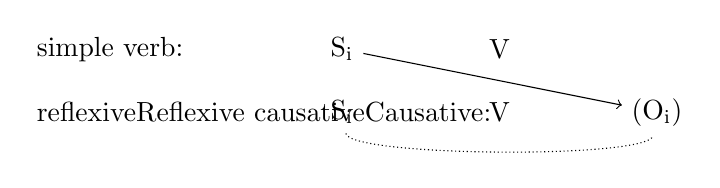
\begin{tikzpicture}[node distance=2cm]

% nodes
\node (x) [anchor=west] at (0, .8) {simple verb:};
\node (x) [anchor=west] at (0, 0) {reflexive\is{Reflexive} causative\is{Causative}:};

\node (S1) at (4, .8) {S\textsubscript{i}};
\node (V1) at (6, .8) {V};
\node (S2) at (4, 0) {S\textsubscript{i}};
\node (V2) at (6, 0) {V};
\node (O) at (8, 0) {(O\textsubscript{i})};

% arrows
\draw [->] (S1) -- (O) ;
\draw[densely dotted] (S2)  to[out=-80,in=-100,distance=.3cm] (O) ;
  

\end{tikzpicture}


}
% \todo[inline]{Add arrow and dotted curve.}

This is illustrated in the following two pairs of examples, first with \textit{riro} ‘become’, then with \textit{takataka} ‘gather’:

\ea\label{ex:8.240}
\gll Ko \textbf{riro} {\ꞌ}ā pē he vārua {\ꞌ}ā. \\
\textsc{prf} become \textsc{cont} like \textsc{pred} spirit \textsc{ident} \\

\glt 
‘He had become like a spirit.’ \textstyleExampleref{[R310.268]} 
\z

\ea\label{ex:8.241}
\gll He uru Taŋaroa ki roto i te vai, he \textbf{haka} \textbf{riro} pa he kahi. \\
\textsc{ntr} enter Tangaroa to inside at \textsc{art} water \textsc{ntr} \textsc{caus} become like \textsc{pred} tuna \\

\glt 
‘Tangaroa entered into the water and turned himself into a tuna.’ \textstyleExampleref{[Fel-046.020]}
\z

\ea\label{ex:8.242}
\gll He oho mai he \textbf{takataka} {\ꞌ}i te hare o te hānautama. \\
\textsc{ntr} go hither \textsc{ntr} gather:\textsc{red} at \textsc{art} house of \textsc{art} pregnant \\

\glt 
‘They came and gathered in the house of the mother-to-be.’ \textstyleExampleref{[Ley-9-55.024]}
\z

\ea\label{ex:8.243}
\gll He \textbf{haka} \textbf{takataka} {\ꞌ}i tū hare era o tū taŋata era. \\
\textsc{ntr} \textsc{caus} gather:\textsc{red} at \textsc{dem} house \textsc{dist} of \textsc{dem} man \textsc{dist} \\

\glt
‘They gathered in the house of that man.’ \textstyleExampleref{[R352.079]} 
\z

These ‘implicit reflexives\is{Reflexive}’ are part of a larger phenomenon: in many cases, causatives do not add a new argument to the verb, so the argument structure of the root is not modified. What addition of \textit{haka} does in such cases, is adding a semantic element, usually an element of agentivity\is{Agentivity}, activity or intensity. For example, while \textit{{\ꞌ}ui} means ‘to ask’, \textit{haka {\ꞌ}ui} is used in the sense ‘to ask persistently and/or repeatedly, to inquire’. Both verbs have the same argument structure, but the causative\is{Causative} verb is more intensive.

\ea\label{ex:8.244}
\gll He \textbf{haka} \textbf{{\ꞌ}ui} mai te aŋa e te ŋā poki repahoa ō{\ꞌ}oku pē nei ē...\\
\textsc{pred} \textsc{caus} ask hither \textsc{art} do \textsc{ag} \textsc{art} \textsc{pl} child friend \textsc{poss.1sg.o} like \textsc{prox} thus\\

\glt
‘My friends kept asking me as follows...’ \textstyleExampleref{[R380.042]} 
\z

\textit{{\ꞌ}Ava{\ꞌ}ava} means ‘to be at a distance’ or ‘to move away, to withdraw’; \textit{haka {\ꞌ}ava{\ꞌ}ava} also has the latter sense, but underlines that the act of withdrawing is volitional. Compare the following pair of examples:

\ea\label{ex:8.245}
\gll Te naonao {\ꞌ}ina he \textbf{{\ꞌ}ava{\ꞌ}ava} rahi mai tō{\ꞌ}ona kona poreko. \\
\textsc{art} mosquito \textsc{neg} \textsc{ntr} distance\_oneself much from \textsc{poss.3sg.o} place born \\

\glt 
‘The mosquito does not go far from its breeding place.’ \textstyleExampleref{[R535.065]} 
\z

\ea\label{ex:8.246}
\gll {\ꞌ}Ina koe ko \textbf{haka} \textbf{{\ꞌ}ava{\ꞌ}ava}. \\
\textsc{neg} \textsc{2sg} \textsc{neg.ipfv} \textsc{caus} distance\_oneself \\

\glt
‘Don’t go away.’ \textstyleExampleref{[R482.045]} 
\z

The same phenomenon can be observed with adjectives. While \textit{haka} + adjective may be a true causative\is{Causative}, expressing that the property is brought about by an external Agent (see (\ref{ex:8.228}–\ref{ex:8.229}) above), it may also express that the subject reaches a state or acquires a property through intentional action. A few examples:

\ea\label{ex:8.246a}
\begin{tabbing}
xxxxxxx \= xxxxxxxxxxxxxxxx \= xxxxxxxxxxxx \= xxxxxxxx \kill
\textit{hāhine} \> ‘to be/draw near’ \> \textit{haka hāhine} \> ‘to approach (volitionally)’\\
\textit{aŋiaŋi} \> ‘to be sure’ \> \textit{haka aŋiaŋi} \> ‘to make sure, verify’\\
\textit{rohirohi} \> ‘to be tired’ \> \textit{haka rohirohi} \> ‘to tire oneself out’
\end{tabbing}
\z

\ea\label{ex:8.247}
\gll He \textbf{haka} \textbf{hāhine} atu o Hotu ki te {\ꞌ}ōpani o tū piha era. \\
\textsc{ntr} \textsc{caus} near away of Hotu to \textsc{art} door of \textsc{dem} room \textsc{dist} \\

\glt 
‘Hotu approached the door of the room.’ \textstyleExampleref{[R301.121]} 
\z

\ea\label{ex:8.248}
\gll Ko haka\_tiu {\ꞌ}ā te repa mai {\ꞌ}uta ki te vaikava  mo \textbf{haka} \textbf{aŋiaŋi} ana ai ko tano {\ꞌ}ā mo hakahonu.\\
\textsc{prf} watch \textsc{cont} \textsc{art} young\_man from inland to \textsc{art} sea  for \textsc{caus} certain:\textsc{red} \textsc{irr} exist \textsc{prf} correct \textsc{cont} for bodysurf\\

\glt 
‘The young men observe the sea to make sure whether the conditions are fit for surfing.’ \textstyleExampleref{[R431.001]} 
\z

\textit{Haka} + adjective or adverb\is{Adverb} may also indicate that the subject acts in a way characterised by the root. As \REF{ex:8.250} shows, this may involve simulating a certain characteristic.\footnote{\label{fn:457}Cf. \citet[14]{Moyle2011} about “similative use” of the causative prefix in \ili{Takuu}.}

\ea\label{ex:8.249}
\gll E \textbf{haka} \textbf{koro{\ꞌ}iti} koe ana vānaŋa mai. \\
\textsc{exh} \textsc{caus} softly \textsc{2sg} \textsc{irr} speak hither \\

\glt 
‘Speak softly (lit. make softly when you speak)!’ \textstyleExampleref{[R408.046]} 
\z

\ea\label{ex:8.250}
\gll Te tire e haŋa rō {\ꞌ}ā mo \textbf{haka} \textbf{{\ꞌ}ata} \textbf{māramarama} i a rāua. \\
\textsc{art} Chile \textsc{ipfv} want \textsc{emph} \textsc{ident} for \textsc{caus} more intelligent \textsc{acc} \textsc{prop} \textsc{3pl} \\

\glt 
‘The Chileans want to pass themselves off as smarter.’ \textstyleExampleref{[R428.006]} 
\z

\subsection{Lexicalised causatives}\label{sec:8.12.5}

A number of \textit{haka} forms have a meaning which cannot quite be predicted from the meaning of the root. Some examples:

\ea
\begin{tabbing}
xxxxxxxxx \= xxxxxxxxxxxxx \= xxxxxxxxxxxxx \= xxxxxxxx \kill
\textit{pāpa{\ꞌ}i} \>  ‘to~write’ \>  \textit{haka~pāpa{\ꞌ}i} \>  ‘to~enrol’\\
\textit{{\ꞌ}omo{\ꞌ}omo} \>  ‘to~suck’ \>  \textit{haka~{\ꞌ}omo{\ꞌ}omo} \>  ‘to~breastfeed’\\
\textit{rivariva} \>  ‘good’ \>  \textit{haka~rivariva} \>  ‘to~improve;~to~prepare’\\
\textit{roŋo} \>  ‘message’ \>  \textit{hakaroŋo} \>  ‘to~listen;~to~perceive’
\end{tabbing}
\z

Another example is found in \REF{ex:8.248} above: \textit{haka honu} ‘bodysurfing’ is a lexicalised causative\is{Causative} from \textit{honu} ‘turtle’. The same sentence also contains the verb \textit{hakatiu} ‘to watch’; even though this is formally a causative, there is no word \textit{tiu} in the Rapa Nui lexicon. There are a few more \textit{haka} forms for which the root as such is not a Rapa Nui word. This includes two very common words: \textit{\mbox{haka{\ꞌ}ou}} ‘again’, \textit{hakarē} ‘to leave (abandon; permit)’. 

\subsection{The causative prefix with nouns}\label{sec:8.12.6}

When the root of the \textit{haka} construction is a noun, the causative\is{Causative} expresses an action which is in some way characterised by the noun. The noun may be the product of the action: \textit{haka N} = ‘to cause the object to be N, to make something into N’, or more generally ‘to make/create N’:

\ea\label{ex:8.251}
\gll He tītiŋi i te ivi ra{\ꞌ}e, he \textbf{haka} \textbf{parehe}.\\
\textsc{ntr} \textsc{pl}:crush \textsc{acc} \textsc{art} bone first \textsc{ntr} \textsc{caus} piece\\

\glt 
‘He crushed the first bone into pieces.’ \textstyleExampleref{[Mtx-3-01.199]}
\z

\ea\label{ex:8.252}
\gll {\ꞌ}I te mahana maha i \textbf{haka} \textbf{kāuŋa} tahi era te ŋā poki. \\
at \textsc{art} day four \textsc{pfv} \textsc{caus} line all \textsc{dist} \textsc{art} \textsc{pl} child \\

\glt
‘On Thursday all the children lined up (formed a line).’ \textstyleExampleref{[R334.139]} 
\z

Other relationships to the noun are possible, whether conventional or creative. In \REF{ex:8.253} the noun refers to something used in the action, or something characterising the direct object as a result of the action. In \REF{ex:8.254} the noun is used in a figurative way (cf. \ili{English} ‘cheeky’). 

\ea\label{ex:8.253}
\gll E \textbf{haka} \textbf{tiare} rō {\ꞌ}ana i a rāua. \\
\textsc{ipfv} \textsc{caus} flower \textsc{emph} \textsc{cont} \textsc{acc} \textsc{prop} \textsc{3pl} \\

\glt 
‘They have adorned themselves with flowers.’ \textstyleExampleref{[R416.415]} 
\z

\ea\label{ex:8.254}
\gll {\ꞌ}Ina ho{\ꞌ}i koe ko \textbf{haka} \textbf{{\ꞌ}āriŋa} ki tu{\ꞌ}u māmā ena.\\
\textsc{neg} indeed \textsc{2sg} \textsc{neg.ipfv} \textsc{caus} face to \textsc{poss.2sg.o} mother \textsc{med}\\

\glt 
‘Don’t be insolent to your mother.’ \textstyleExampleref{[R103.065]} 
\z

\subsection{Lexical causatives}\label{sec:8.12.7}

The term \textit{lexical causative}\is{Causative} refers to a situation where there are two lexemes, unrelated in form, one of which is semantically the causative\is{Causative} of the other. (\citealt[248]{Dixon2012}.) 

There are very few lexical causatives in Rapa Nui; the following two are possible candidates.

\subparagraph{\ref{sec:8.12.7}.1} \textit{Hāŋai} ‘to feed’ can be considered a causative\is{Causative} of \textit{kai} ‘to eat’. Apart from the obvious semantic relationship between the two, there are two reasons to assume a causative\is{Causative} relationship between the two:

%\setcounter{listWWviiiNumvileveli}{0}
\begin{enumerate}
\item 
The morphological causative\is{Causative} \textit{haka kai} does not occur; whenever a causative\is{Causative} of \textit{kai} is called for, \textit{hāŋai} is used. 

\item 
The arguments of \textit{hāŋai} show the same patterns of case-marking as morphological causatives. When the object of eating (the food) is not expressed or implied, the causee (the eater) is expressed as direct object:

\end{enumerate}

\ea\label{ex:8.255}
\gll I tu{\ꞌ}u era he hāŋai \textbf{i} \textbf{a} \textbf{Ure} ka oti rō. \\
\textsc{pfv} arrive \textsc{dist} \textsc{ntr} feed \textsc{acc} \textsc{prop} Ure \textsc{cntg} finish \textsc{emph} \\

\glt
‘When she arrived, she fed Ure completely.’ \textstyleExampleref{[R310.291]} 
\z

But when the object of eating is implied, the causee is marked with \textit{ki}.\footnote{\label{fn:458}There are no examples in the corpus where the causee and the object of eating are both expressed.}

\ea\label{ex:8.256}
\gll He to{\ꞌ}o mai tū kai era, he hāŋai \textbf{ki} \textbf{tū} \textbf{ŋā} \textbf{matu{\ꞌ}a} era o Tiare. \\
\textsc{ntr} take hither \textsc{dem} food \textsc{dist} \textsc{ntr} feed to \textsc{dem} \textsc{pl} parent \textsc{dist} of Tiare \\

\glt
‘They took the food and fed (it) to Tiare’s parents.’ \textstyleExampleref{[R238.009]} 
\z

Not all instances of \textit{hāŋai} can be considered as lexical causatives\is{Causative}, though: the verb is also used in the sense ‘to raise/tend (animals); to raise/rear (children)’.

\subparagraph{\ref{sec:8.12.7}.2} Another possible lexical causative\is{Causative} is \textit{tiŋa{\ꞌ}i} (var. \textit{tiaŋi}) ‘to kill’, causative\is{Causative} of \textit{mate} ‘to die’:

\ea\label{ex:8.257}
\gll He tiŋa{\ꞌ}i i te taŋata, i te vi{\ꞌ}e, i te poki.\\
\textsc{ntr} kill \textsc{acc} \textsc{art} man \textsc{acc} \textsc{art} woman \textsc{acc} \textsc{art} child\\

\glt
‘They killed men, women and children.’ \textstyleExampleref{[Mtx-3-01.250]}
\z

Apart from the sense ‘to kill’, \textit{tīŋa{\ꞌ}i} also has a different (though obviously related) sense: ‘to strike, hit’. Note also that the sense ‘to kill’ is also expressed occasionally by the morphological causative\is{Causative} \textit{haka mate}.

\subparagraph{\ref{sec:8.12.7}.3} A number of causative\is{Causative} verbs were borrowed as a whole from \ili{Tahitian}\is{Tahitian influence}. These are clearly recognizable as borrowings\is{Borrowing}, as they start with \textit{ha{\ꞌ}a-}\is{haa- (causative)@ha{\ꞌ}a- (causative)} ({\textless} Tah. \textit{fa{\ꞌ}a}{}-) rather than \textit{haka}. Most of these are isolated lexical items, the root of which does not occur on its own in Rapa Nui: \textit{ha{\ꞌ}atura} ‘to obey, respect’ (Tah. \textit{tura} ‘respect.N’); \textit{ha{\ꞌ}ati{\ꞌ}a} ‘to permit’ (Tah. \textit{ti{\ꞌ}a} ‘to stand’). For most of these words, it is not at all obvious that \textit{ha{\ꞌ}a-} has a causative\is{Causative} sense in Rapa Nui.

For a few \textit{ha{\ꞌ}a-} forms, however, the root as such was also borrowed into Rapa Nui: \textit{{\ꞌ}ī} ‘to be full’, \textit{ha{\ꞌ}a{\ꞌ}ī} ‘to fill’. As \textit{ha{\ꞌ}a-} is not a productive prefix in Rapa Nui, \textit{ha{\ꞌ}a{\ꞌ}ī} can be considered as a lexical causative\is{Causative} of \textit{{\ꞌ}ī}, rather than a form derived through prefixation of \textit{ha{\ꞌ}a-}.
\is{Causative|)}

\section{Conclusions}\label{sec:8.13}
\largerpage[2]
This chapter has explored the expression of core constituents of verbal clauses.

Rapa Nui patterns with other Polynesian languages in that the S/A argument is marked with \textit{e} or unmarked, while the O argument is marked with \textit{i} or unmarked. However, the resulting case marking patterns are different from those in other languages. At first sight Rapa Nui may seem to have ergative traits, but a close analysis shows that the language is unambiguously accusative. The case marking patterns which seem to deviate from regular accusativity can be explained by the following features:

\begin{itemize}
\item 
obligatory omission of case markers in certain noun phrases, e.g. those containing a prenominal numeral;

\item 
extensive use of the agentive marker \textit{e}, both in transitive and intransitive clauses;

\item 
omission of the object marker \textit{i} in certain clause types;

\item 
a passive construction which is somewhat inconspicuous because of the absence of passive morphology.

\end{itemize}

Agent marking is determined by an interplay of heterogenous factors: syntactic (preverbal subjects are always unmarked), lexico-semantic (some verbs show a strong preference for \textit{e-}marked Agents) and pragmatic (Agents which start to act, tend to be \textit{e}{}-marked). The same is true for object marking: the object marker is omitted under certain conditions, which may be syntactic (OV clauses), lexico-semantic (with certain verbs) or pragmatic (non-salient objects).

Rapa Nui has a passive construction, in which the Patient is expressed as subject while the Agent is an optional oblique (but without morphological changes in the verb). In fact, passivisation in Rapa Nui is part of a wider phenomenon: several (groups of) verbs exhibit variation in argument assignment. For example, the verb \textit{{\ꞌ}ī} ‘to be full’ has two argument structures, with the Container and the Substance as subject, respectively. Variable argument structure can also be observed with transfer verbs like ‘to feed’ and ‘to throw’: with these verbs, either the Patient or the Goal/Recipient is expressed as direct object; the other argument is expressed as an oblique. When the Patient is oblique, it is marked as an instrument (‘he threw the enemy with a spear’). 

Another argument-related operation is the addition of an external Agent to intransitive verbs; this Agent is marked with the preposition \textit{i}.

Rapa Nui has a number of different comitative constructions (‘A with B’). In most of these, a comitative marker is used, followed by the prominence \textit{ko}; this marker is often a plural pronoun (‘Makemake they \textit{ko} Haua’) or collective marker (‘the people together \textit{ko} the priest’). These comitative markers are used in an inclusory way: their number corresponds the total set of referents of both noun phrases. Similar are constructions with comitative sense – but without a comitative marker – in which the first noun phrase is an inclusory pronoun: ‘we \textit{ko} the child’, meaning ‘the child and~I’.

\largerpage[2]
The final topic of this chapter is causativisation. Causativisation is very common in Rapa Nui; moreover, it is very versatile: 

\begin{itemize}
\item 
it can be applied to any verbal predicate and is occasionally applied to nouns as well; 

\item 
it indicates varying types of causation, both direct (‘he made me do it’) and indirect (‘he let me do it, helped me to do it’);

\item 
while a prototypical causative adds an external Agent to the event, some causatives in Rapa Nui do not change the argument structure of the verb, but add an element of intensity or agentivity.

\end{itemize}
\is{Clause!verbal|)}
